\documentclass[12pt,BCOR=1cm,bibliography=totoc]{thesis}
\pdfminorversion=5 
\pdfcompresslevel=9 
\pdfobjcompresslevel=3
%\usepackage{showframe}

%\KOMAoptions{headings=small}
%\addtokomafont{disposition}{\rmfamily\mdseries}
%\renewcommand*{\contentsname}{Table of Contents}
%\setkomafont{chapterprefix}{\rmfamily\Large\bfseries}


% customize chapter format:
\KOMAoption{headings}{twolinechapter}
\renewcommand*\chapterformat{\color{blue}{Chapter \thechapter}\vspace{-0.6cm}}%\autodot

% customize dictum format:
\setkomafont{dictumtext}{\itshape\small}
\setkomafont{dictumauthor}{\tiny}
\renewcommand*\dictumwidth{0.5\linewidth}
\renewcommand*\dictumauthorformat[1]{--- #1}
\renewcommand*\dictumrule{}


\usepackage{float}
\usepackage{pdfpages}

%*****************************************************************************
\graphicspath{ {figures/} }

%** new commands ******************************************************
%!TEX root = myThesis.tex
%!TEX encoding = UTF-8 Unicode

%***************************************************************************************************
% create smaller pdf
% http://tex.stackexchange.com/questions/14429/pdftex-reduce-pdf-size-reduce-image-quality

%  gs -sDEVICE=pdfwrite -dCompatibilityLevel=1.4 -dPDFSETTINGS=/prepress -dNOPAUSE -dQUIET -dBATCH -sOutputFile=small.pdf Doktorarbeit.pdf

%  gs -sDEVICE=pdfwrite -dCompatibilityLevel=1.4 -dPDFSETTINGS=/ebook -dNOPAUSE -dQUIET -dBATCH -sOutputFile=small.pdf Doktorarbeit.pdf

% -dPDFSETTINGS=/screen   (screen-view-only quality, 72 dpi images)
% -dPDFSETTINGS=/ebook    (low quality, 150 dpi images)
% -dPDFSETTINGS=/printer  (high quality, 300 dpi images)
% -dPDFSETTINGS=/prepress (high quality, color preserving, 300 dpi imgs)
% -dPDFSETTINGS=/default  (almost identical to /screen)
%***************************************************************************************************


% settings -------------------------------------------------------------------
%try this to fix the margin problem
%http://tex.stackexchange.com/questions/10128/two-sided-document-reverse-page-margins-for-hardcopy
%***************************************************************************************************

\usepackage{mathtools} %for the dcases environment
%*****************************************************************************
\setlength{\marginparwidth}{0pt}

\newenvironment{myCompactItemize}
{ \begin{itemize}
    \setlength{\itemsep}{0pt}
    \setlength{\parskip}{0pt}
    \setlength{\parsep}{0pt}     }
{ \end{itemize}                  } 

% 'text' shortcuts -----------------------------------------------------------
\newcommand{\etal}{\textit{et al.\ }}
\newcommand{\kmeans}{$k$--{\ttfamily means} }
\newcommand{\kmeanspp}{$k$--{\ttfamily means++} }
\newcommand{\art}{\textit{i}{\scshape ArteC} }

% math stuff -----------------------------------------------------------------
\DeclareMathOperator{\sgn}{sgn}
\DeclareMathOperator*{\argmin}{arg\,min}
\newcommand{\s}[2]{\left\langle #1,#2\right\rangle} % scalar product
\newcommand{\n}[1]{\left\|#1\right\|}  							% norm
\newcommand{\abs}[1]{\left |#1\right |} 						%abs, magnitude


%commented out because it causes  the error:
%too many math alphabets used in version normal
%\usepackage{bm}
%\renewcommand{\vec}[1]{\ensuremath{\bm{#1}}}
%\newcommand{\matx}[1]{\ensuremath{\bm{#1}}}     		%matrix notation (ISO complying version)

\renewcommand{\vec}[1]{\ensuremath{\mathbf{#1}}} 	%vector notation
\newcommand{\matx}[1]{\ensuremath{\mathbf{#1}}} 		% matrix notation


%$\begin{bmatrix*}[r]
  %-1 & 3 \\
  %2 & -4
 %\end{bmatrix*}
%$

% environment redefenitions --------------------------------------------------
\newtheorem{defn}{Method}%{\bfseries}{\itshape}
\theoremstyle{definition} %plain | definition | remark
\newtheorem{definition}{Definition}

%shorthand for the nomenclature that prints the symbol/abbreviation and generates a list entry at the same time.
\newcommand*{\nom}[2]{#1\nomenclature{#1}{#2}}
%example: \nom{EST}{Eastern Standard Time}
%\nom{}{}

%\def\mydate{\leavevmode\hbox{\the\year-\twodigits\month-\twodigits\day}}
\def\mydate{\leavevmode\hbox{\the\year\twodigits\month\twodigits\day}}
\def\twodigits#1{\ifnum#1<10 0\fi\the#1}

%** listings settings ******************************************************

\lstset{basicstyle=\footnotesize\ttfamily,breaklines=true}
\lstset{framextopmargin=50pt,frame=bottomline}
\lstset{showstringspaces=false}%do not use "squat-u" symbole for space

\lstdefinelanguage{XML}{ 
    columns=fullflexible, 
    basicstyle=\footnotesize\ttfamily, 
    commentstyle=\ttfamily\color{green!50!black}, 
    morestring=[s]{"}{"}, 
        alsoletter={ },
    morecomment=[s]{?}{?}, 
    morecomment=[s]{!--}{--}, 
    morecomment=[s]{!DOCTYPE}{]}, 
    moredelim=[s][\color{black}]{>}{<}, 
    moredelim=[s][\bfseries\color{black}]{\ }{=}, 
    stringstyle=\color{blue}, 
    identifierstyle=\bfseries\color{violet} 
} 

\lstdefinelanguage{terCmd}{
        basicstyle=\footnotesize\ttfamily, 
    sensitive=false,
    alsoletter={.},
    alsoletter={\$},
    morestring=[s]{"}{"}, 
    stringstyle=\color{blue}, 
    morestring=[s]{'}{'}, 
    %stringstyle=\color{violet}, 
    moredelim=[s][\color{red}]{<}{>},
    moredelim=[s][\color{blue}]{[}{]},
    %  moredelim=[is][\color{orange}]{:}{:},
    keywords=[10]{roslaunch,model,rospack,find,source,cd,sudo,usermod,chmod},
    keywordstyle=[10]{\color{magenta}},
}

\lstset{language=C++,
    basicstyle=\footnotesize\ttfamily,
    keywordstyle=\color{blue}\ttfamily,
    stringstyle=\color{red}\ttfamily,
    commentstyle=\color{teal}\ttfamily,
    morecomment=[l][\color{magenta}]{\#}
}

\usepackage{tcolorbox}
\tcbuselibrary{skins,breakable}
\usetikzlibrary{shadings,shadows}

\newenvironment{mynotebox}[1]{%
    \tcolorbox[beamer,width=\textwidth,
    noparskip,breakable,
    colback=red!1,colframe=red!50,%
    colbacklower=red!5,%
    title=\textbf{#1}]}%
{\endtcolorbox}

%------------------------------------------------------------------------------

\begin{document}
\pagestyle{empty}

\begin{titlepage}
\centering
  \includegraphics[width=0.15\textwidth]{myFrontMatter/figures/zuLogo} \qquad 
\includegraphics[width=0.2\textwidth]{myFrontMatter/figures/engLogo}\\
 {\usekomafont{titlehead}   Zagazig University, Faculty of Engineering,\\
     Mechatronics Program}

    \vskip 8ex
    {\LARGE\usekomafont{title} {\LARGE Implementation of KUKA Robotic Arm in Industrial 3D Intelligent Milling }    \vskip .5ex
         {\normalsize Deployment of industrial KUKA robot in CNC machining and visual servoing through Kinect interfacing on ROS}}
    \vskip 3ex
     \emph{Graduation project for the degree Bachelor of Science (B.Sc.)} 
     \vskip .3ex
     \emph{Submitted to  Mechatronics Program, Faculty of Engineering, Zagazig University, Egypt}
     
     \vskip 8ex
    {\usekomafont{subtitle} By}
    \vskip 1ex
    {\usekomafont{author} 
        Ahmed Emam\\
        Ahmed Saeed\\
        Donna Mustafa\\
        Dua’a Samir\\
        Hoda Mahmoud\\
        Reeham Mohamed\\}

    \vskip 6ex
    {\usekomafont{subtitle} Supervisors}
    \vskip 1ex
%    \emph{Asst. Prof. Dr.Ing.} {\usekomafont{author}\bfseries Mohammed Nour A. Ahmed}
%    \vskip 1ex
%    \emph{Computer and Systems Engineering Dept., Faculty of Engineering, Zagazig University, Zagazig, Egypt}
%   \vskip 1ex
%       \emph{Asoc. Prof. Dr.} {\usekomafont{author}\bfseries Ahmed Hamdy Hassanien}
%   \vskip 1ex
%   \emph{Mechanical Engineering Dept., Faculty of Engineering, Zagazig University, Zagazig, Egypt}
%   
   \begin{tabular}{cc}
               \emph{Asst. Prof. Dr.Ing.}                &   	               \emph{Asst. Prof. Dr.}                 \\
 {\usekomafont{author}\bfseries Mohammed Nour A. Ahmed } &   	{\usekomafont{author}\bfseries Ahmed H. Hassanien} \\
      \emph{Computer and Systems Engineering Dept.}      &   	         \emph{Mechanical Engineering Dept.}          \\
           \multicolumn{2}{c}{Faculty of Engineering, Zagazig University, Zagazig, Egypt}
   \end{tabular} 

   \vfill
    July, 2017
\end{titlepage}
%% Rückseite der Titelseite %%%%%%%%%%%%%%%%%%%%%%%%%%%%%%%%%%%%%%%%%%%
\newpage
{Graduation Project Report submitted to\\
    \textbf{Zagazig University, faculty of Engineering, Mechatronics Program}, Zagazig, Egypt\\
    in partial fulfillment of the requirements for the degree \\
    Bachelor of Science in Engineering (\textbf{B.Sc.})\\
    \textcopyright 2017

%    \vspace{1cm}
    {\footnotesize
        Copyright \textcopyright 2017 Asst. Prof. Dr.Ing. Mohammed Nour Abdelgwad Ahmed as part of his course work and learning material. All Rights Reserved. 
        Where otherwise noted, this work is licensed under 
        \href{https://creativecommons.org/licenses/by-nc-sa/4.0/}{ a Creative Commons Attribution-NonCommercial-ShareAlike 4.0 International License}.}\\
    
\includegraphics[width=0.15\textwidth]{myFrontMatter/figures/byncsa}}\\

%    \vspace{2cm}
{\textbf{Date of Presentation}\\
    15. July 2017\\
    
    
    
     {\textbf{Project Team Members}\\
             \noindent\begin{tabular}{ll}
        Ahmed Emam&        Ahmed Saeed\\
        Donna Mustafa&        Dua’a Samir\\
        Hoda Mahmoud& Reeham Mohamed
            \end{tabular}
    
    \textbf{Supervisors}\\
         Asst. Prof. Dr.Ing. \textbf{Mohammed Nour A. Ahmed}\\
    {\itshape \footnotesize
                 (Project Leader)\\
        Computer and Systems Engineering Department,\\
        Faculty of Engineering, Zagazig University, Egypt}\\~\\
    	Asst. Prof. Dr. \textbf{Ahmed Hamdy Hassanien}\\
    {\itshape\footnotesize Mechanical Engineering Department, \\
    	Faculty of Engineering, Zagazig University, Egypt}\\
   
    
  
    \textbf{Defense Committee}\\
    \noindent\begin{tabular}{p{4.1in}p{2.2in}}
Prof. Dr. \textbf{Nabil H. Mostafa}  & \dotfill \\
\emph{\footnotesize Mechanical Engineering Dept., Faculty of Engineering, Zagazig University} & signature\\[4ex]% adds space between the two sets of signatures
Asst. Prof. Dr. \textbf{Mohamed Talaat} & \dotfill \\
\emph{\footnotesize Electric Power Engineering Dept., Faculty of Engineering, Zagazig University} & signature\\[4ex]
Asst. Prof. Dr.Ing. \textbf{Mohammed Nour A. Ahmed} & \dotfill \\
\emph{\footnotesize Computer and Systems Engineering Dept., Faculty of Engineering, Zagazig University} & signature\\[4ex]
Asst. Prof. Dr. \textbf{Ahmed Hamdy Hassanien} & \dotfill \\
\emph{\footnotesize Mechanical Engineering Dept., Faculty of Engineering, Zagazig University} & signature
    \end{tabular}
\vfill
{\tiny Revision SVN.198.50.\mydate }

%\maketitle
%------------------------------------------------------------------

\frontmatter 
\pagestyle{fancy}
\addcontentsline{toc}{chapter}{Dedication}
%\dedication{

    \vspace*{0.35\textheight}
    \begin{center}
    {\LARGE In memory of \textbf{Ahmed Emam}}
    \end{center}

        
%}{\Large }
\markboth{Abstract}{}
\chapter*{Abstract}\label{ch:abstract}
\addcontentsline{toc}{chapter}{Abstract}
%%\begin{abstract}
%The first industrial revolution marked the transition to new manufacturing processes in eighteenth century, which is arguably similar to the transition introduced by the use of robotic manipulators in different industrial aspects in the late twentieth century. This project is motivated by the major developments in the industrial sector thanks to robots, especially in machining processes. Robots offer more flexibility, cost reduction and higher level of details, all of which are essential characteristics to any successful industry. Although these characteristics can be obtained by conventional CNC machines, however, the level and rate of production differ on larger scales, in favor of the robots. 
%
%The main problem can be summarized in Four points; accuracy, ease of use, flexibility and safety, and the solution to these problems defines the scope of our project. As for accuracy, it is obtained by implementing the robot itself, which offers multiple-axes movement, enabling the possibility for higher level of details than the conventional CNC machines. Ease of use is demonstrated in the user-friendly robot interface that enables the implementation of projects easily and without the need to multiple machines or tasks to deliver the final results. Flexibility is provided through the multiple programmable interfaces that offer multiple methods of control; Inline programming through KUKA’s smartPAD, offline programming through converting G-codes from CAD files into KRL and ROS. Safety is increased in the work space of the robot by introducing a vision based safety system that reduces the robot’s operating speed when someone enters this work space.
%
%The results of the aforementioned methods and applications are diverse, offering milling in multiple dimensions and thus widening the scope of final products. In addition to introducing further control methods, which opens up new doors towards further developments and applications that were not applicable earlier.
%%\end{abstract}
\setlength{\parindent}{1em}
  
This report describes the first commissioning process, and the deployment of both industrial and research applications on KUKA KR6 R900 sixx at Zagazig University. This project is a Bachelor graduation project submitted to the Mechatronics Program on 2017.%, which was purchased through the Tempus project "JIM2L", lead by Hochschule Bochum three years before writing this report.

The project work--flow included three major phases: \textbf{Commissioning the robot}- starting from base setting and mastering the robot to installing different end-effectors and making complete programs,  \textbf{Implementation of an industrial application}- through developing post-processing tools to convert any conventional G-Code into KUKA Robot Language (KRL) and use the robot for 2D drawing and 3D milling, and \textbf{ Implementation of two research applications} related to visual servoing- through using Kinect interfacing on ROS to guide the robot with hand gestures and provide human-safe operating zone where the robot stops when a human approaches, which was made possible after developing an API to control the robot directly from any PC.

\vspace{2cm}
\noindent\textbf{Keywords:} KUKA Robot, KUKA Robot Language (KRL), G-Code, visual servoing, Kinect, ROS, Robot-human-safe operating zone, Robot API.
 
 
%\input{chapters/abstractAr}
\markboth{Acknowledgements}{}

\chapter*{Acknowledgements}
\addcontentsline{toc}{chapter}{Acknowledgements}
%
%This graduation project consumed huge amount of work, research and dedication. Still, accomplishment would not have been possible if we did not have a support of many individuals. Therefore we would like to extend our sincere gratitude to all of them.
%
%%advisor
%First of all, we would like to sincerely thank our advisors Dr.Ing. Mohammed Nour and Dr Ahmed Hamdy. They gave us the opportunity to work on great ideas with great people . When needing someone for the
%discussion of any problem, ..... was always there and also solved a lot of .......... problems for/with us.
%
%
%
%we are also grateful to our friends and colleagues, XYZ, ABC, and UVW. For getting into the basics of this project, we had a lot of support by XYZ who raised our first interest during the initial part of this work. ABC helped us a lot with the .........  and experiments. UVW helped so much in ......... We are indebted to ........... for making ............. easier to understand and to introduce ........ to us. 
%
%%Experiments: 
%we express our warm thanks to ......, ............., and ............. for making the ............. robot available to us and the time they spend assisting us to carry out the field experiments. Without their superior knowledge and experience, the experiments would not have that like in quality of outcomes, and thus their support has been essential. In addition, we wish to express our sincere gratitude to ............. for helping when we had questions as well as frustrations.
%
%
%We would like to thank all the numerous people in the internet who ask questions and provide answers for programming problems (specifically in ROS) and for the very useful code and tools they share with others.
%
%%family and friends
%we would like to most importantly acknowledge the effort of our families, who encouraged us to pursue higher education and support us through the difficulties associated with such a goal even when we was not sure we would make it through. 
%
%Last but not least, we would like to thank our friends for always encouraging us onwards. We can
%never thank them enough for their love and faith.
%
We would like to express our deepest gratitude and appreciation to all those who made it possible to complete this project: our project supervisors- prof. Mohamed Nour Abdelgawad and Prof. Ahmed Hamdy- for their support and guidance throughout the project,  KUKA Roboter GmbH for their amazing robots, Mechanical Engineering department's professors for providing us with help and guidance, and Zagazig University for funding our project.

We would also like to thank all the numerous people in the Internet who ask questions and provide answers for programming problems (specifically in ROS) and for the very useful code and tools they share with others.

Last but not least, we would like to thank our families and friends for always encouraging us onwards. We can never thank them enough for their love and faith.

\tableofcontents
\listoffigures
\listoftables
%\listofalgorithms
%------------------------------------------------------------------

\mainmatter
\pagestyle{fancy}
%------------------------------------------------------------------

\setchapterpreamble[o]{%
    \dictum[Niccolo Machiavelli, \textit{(Italian writer and statesman, Florentine patriot, author of 'The Prince', 1469-1527)}]{%
        ``There is nothing more difficult to take in hand, more perilous to conduct or more uncertain in its success than to take the lead in the introduction of a new order of things.''}}
\chapter{Introduction}\label{ch:introduction}
%\documentclass{article}
%\usepackage{graphicx}
%
%\begin{document}
%\section{Introduction}
\setlength{\parindent}{1em}
   
Nowadays any kind of modern production use more and more automatic solutions to achieve new goals. That is why automatic systems use in most cases different robot manipulators. Industries that employ robots in a wide variety of applications are the main customers for robot manufacturers. The manipulator market for research applications, on the other hand, is simply too small for the robot manufacturing industry to develop models specifically for such use. While the hardware and mechanical requirements of developed robots are often similar for both industry and research, scientific software requirements are quite different and even contradictory in many aspects. The goal of scientists is to try to gain as much control over the robot as possible, whereas industries seek safe and easy operational interfaces. 

Some of the pioneering companies in the Industrial robotics market are ABB Ltd., Fanuc Corp., Yaskawa Electric Corp., Apex Automation and Robotics, Mistubishi Electric Corp. and KUKA AG. We had the opportunity to work with the latter, KUKA AG, on their model KR6 R900 sixx.
%Over the course of our final year, this project helped increase our knowledge, not only on the main topic, milling and visual servoing, but also on the KUKA platform itself, which is considered an advanced platform widely used in today’s industries. 
\begin{figure}[H]
    \centering
    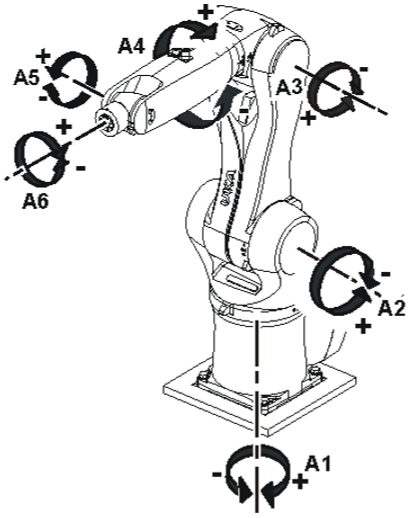
\includegraphics[scale=0.40]{figures/specs6}
     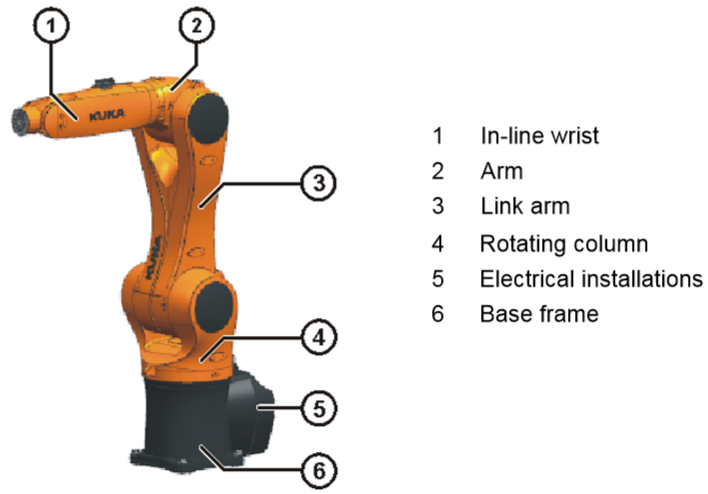
\includegraphics[scale=0.45]{figures/specsc}
    \caption{KUKA KR6 R900 sixx robotic manipulator}
\end{figure}

This robot can carry up to \textbf{6}kg of payload, and reach any point in range of \textbf{900}mm away from its base with \textbf{six} degrees of freedom posing. The robot model name indicates these specifications "KR\textbf{6} R\textbf{900} \textbf{sixx}". It's part of the \textbf{KR AGILUS} series, which includes many other robot varieties for the payload, maximum reach, and the degrees of freedom. 

This robot was purchased three years before starting this project, but no one had commissioned the robot nor installed it properly. We were the first group to use this robot.
 
Before using any industry level robot arm, it first needed to be fixed of a proper- vibration free base setting, then calibrated to get its encoders to work properly. We needed to go through the manuals to learn how to fix, master (calibrate),and program the robot. The design and manufacturing of a base to support the robot during heavy duty operation included performing mathematical calculations based on the robot’s weight and forces to obtain the optimal dimensions and weight for the base, besides performing CAD studies on the manipulator’s body to support the results of the mathematical analysis.

We'd done lots of experiments to learn the syntax of the KRL (KUKA Robot Language). Too much time had been consumed due to lack of resources. We'd found that in addition to robots’ ability to perform several tasks; by adding the desired end-effector and designing the corresponding programming tool, they offer more variations of one task offered by a conventional machine. We'd decided that our project would include two more phases:  \textbf{Implementation of an industrial application}- through developing post-processing tools to convert any conventional G-Code into KUKA Robot Language (KRL) and use the robot for 2D drawing and 3D milling, and \textbf{ Implementation of two research applications} related to visual servoing- through using Kinect interfacing on ROS to guide the robot with hand gestures and provide human-safe operating zone where the robot stops when a human approaches, which was made possible after developing an API to control the robot directly from any PC.	
 
%The milling process witnessed vast development since the early milling machines, known as mills, followed by CNC milling machines and all the way to milling robots. The latter, represented in KUKA robots in our project, can be compared to CNC machines in terms of introducing a computer-based control method, however, milling robots offers more advantages than the conventional CNC machines. One of these advantages is flexibility, because as the needs of manufacturing evolve; robots are proving to be nimble adjusters. 
	
\bigskip
	
%	In addition to robots’ ability to perform several tasks; by adding the desired end effector and designing the corresponding programming tool, they offer more variations of one task offered by a conventional machine. To verify this we can compare CNC milling machines and milling robots. 

%CNC machines offer two-dimensional milling operations, moving either horizontally or vertically with fixed workpiece, resulting in a defined scope of products and processes. Milling robots on the other hand, are able to perform milling in up to six axes, providing rotation and movement in multiple directions. This flexibility can further be improved by providing a movable workpiece fixation, increasing the motion axes to nine.
	
We decided to use the robot in milling, because robots offer ease of use through programming, flexibility, speed, precision, cost reduction, repeatability and some of these robots even offer different mounting choices, as they could be mounted on ceilings and walls not just floors.

We first made a 2D-level post-processor extension on Inkscape software, that automatically converts any drawings and text into KRL code files. These files were transferred to the robot, and when executed, the robot made the exact required task. We'd attached a pen, simulating a laser beam to demonstrate this through drawing. Later, we were able to develop 3D post-processing tools for the 3D milling process. 
%all of this contributed to the current status of milling operations; in terms of final finishing, level of details obtained, rate of production and future possibilities for development. 

	
	
%	The project is inspired by the aforementioned development in the industrial sector. The scope of the project can be summarized in the following three points; firstly, the commissioning and operation of the KUKA KR6 R900 sixx robotic manipulator, which included the installation of the related software and creating a network that facilitates communications with the robot. In addition to software commissioning, hands-on experience with the KUKA robot language (KRL) platform was achieved through learning the basic and advanced forms of KRL, which later helped in the development of software tools that facilitates the main objective of the project; the milling process. 
	
%\smallskip	
%	Secondly, the design and manufacturing of a base to support the robot during heavy duty operation, this included performing mathematical calculations based on the robot’s weight and forces to obtain the optimal dimensions and weight for the base, besides performing CAD studies on the manipulator’s body to support the results of the mathematical analysis. 
	
\medskip
	
	%82Finally, the development of various software tools to achieve the purposes of remotely controlling the robot and milling. These tools include an Inkscape extension for converting 2D G-code to KRL, directly using sketches from Inkscape, an independent toolkit for converting 3 axis G-code to KRL. In addition to Python tools; one Python class for reading and writing system variables, and a Python library for controlling the arm motions from pc. The development also included editing openni\_tracker for publishing uncalibrated person's depth and creating ROS nodes for safety operation distance and visual servoing (hand guiding) for the robot.
	
	%Initially, the project scope was limited to the milling process in addition to minor ideas in the smart development of the workspace, however, over the course of the semester we encountered many problems that required extended research in all the previously mentioned aspects, which eventually led to broadening the scope of the project to include these development tools, both relevant and irr*98 elevant to milling. 

	%\section{References}
	%\begin{enumerate}
%		\item http://www.mmsonline.com/articles/a-new-milling-101-what-milling-is-then-and-now-plus-a-glossary-of-milling-terms
		%\item http://www.sickinsight-online.com/safety-and-more-sick-provides-protection-and-navigation-data-for-kukas-kmr-iiwa/ 
		%\item http://medicaldesign.com/contract-manufacturing/modern-cnc-machining-prescription-product-development 
		%\item http://articles.sae.org/11272/ 
		%\item https://en.wikipedia.org/wiki/Multiaxis\_machining 
		%\item https://en.wikipedia.org/wiki/Milling\_(machining) 	
	%\end{enumerate}
	

%\end{document}
%==============================================================================

%Chapter 2: Base Settings and CAD analysis
%chapter 2 (needs remerge)
\setchapterpreamble[o]{%
    \dictum[Alan Turing, \textit{(British pioneering computer scientist, cryptanalyst,$\cdots$, and philosopher, 1912--1954)}]{%
        ``A computer would deserve to be called intelligent if it could deceive a human into believing that it was human.''}}
\chapter{Base Settings and CAD analysis}\label{ch:BaseSettingsCADAnalysis} %and Related Work
%\documentclass{book}
%\usepackage{graphicx}
%\usepackage{subcaption}
%\usepackage{float}

% Reeham Mohamed Ibrahim
%\begin{document}
%	\begin{chapter}{Chapter 2: Base Settings and CAD analysis}
		\section{Mathematical and CAD analysis}
A solid, strong base was required for a robust and free of vibrations motion of the robot. After discussing different base settings, a simple design that consists of a cylindrical body, that will support the robot, with upper and lower flanges, was chosen.
\vspace{0.5 cm}
\paragraph{Base Structure}
The base body is mainly constructed of:
\begin{enumerate}
\item Two lower flanges:
	\begin{itemize}
	\item[--] 1st flange is screwed to the ground and held strongly by the concrete layer beneath it.
	\item[--] 2nd flange connects the cylindrical body of the base to the previously mentioned flange.
	\end{itemize}

\item The cylindrical body that supports the robot. It’s mounted on the 2nd lower flange to stand still while the robot is operated at full speed.

\item The upper flange which holds the robot and is welded to the cylinder.

\item Ribs: there are four upper and lower ribs evenly distributed on the upper and lower flanges, that helps to support the loads exerted on the cylinder.
\end{enumerate}

\begin{figure}[H]
	\centering
	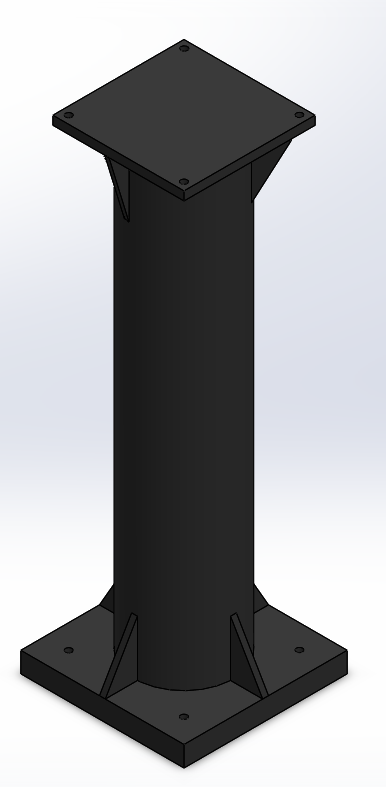
\includegraphics[scale=0.4]{BaseStructure}
	\caption{Base Structure}
\end{figure}

\vspace{0.6 cm}

\subsection {Design of Base Based On Strength}
\paragraph{Base Calculations}
This section discusses the process of calculating the following:
\begin{enumerate}
	\item Cylinder
	\begin{itemize}
		\item[--] Inner and outer diameters of the hollow cylinder.
		\item[--] The height of the cylinder.
	\end{itemize}

    \item Flanges
    \begin{itemize}
    	\item[--] Dimensions (length x width) of the 3 flanges
    	\item[--] The exact locations of the holes through which the bolts will be screwed
    	\item[--] Thickness of the flanges
    \end{itemize}

    \item Bolts
    \begin{itemize}
    	\item[--] Diameters of all bolts used in the installation and mounting of the base.
    \end{itemize}

    \item Ribs
    \begin{itemize}
    \item[--] Dimensions of the triangular ribs (height x width x thickness)
    \end{itemize}
\end{enumerate}

\vspace{0.5 cm}

\subsubsection{The inner and outer diameters of the cylinder}


Since the cylindrical body of the base undergoes different axial and torsional loads, it can be considered as a shaft.

\paragraph{Determining the cylinder diameters}
First attempt was to design the cylinder using the predefined mechanical properties of the commercial materials available in the market, to get the inner and outer diameters. After several weeks of research and calculation, the results were within the range of $10^{-2}$ to $10^{-3}$ mm, which is very small compared to the expected geometry of the cylinder, leaving us to pursue another manner of designing, based on the strength of material.

\paragraph {Design based on strength}
Second design attempt aimed to use the inner and outer diameters of the cylinders available in the market, to check whether the resulting shear stress would exceed the maximum allowable shear the material can withstand or not. The ASME code for this method is:

\begin{equation}
\tau_{allowable} = \frac{16}{\pi d^{3}_{o} (1-k^{4})} \sqrt{(k_{b} M_{b} + \frac{F_{a} d_{o} (1+k^{2})}{8})^{2} + (k_{t} M_{t})^{2}}
\end{equation}
where:
\begin{itemize}
	\item [--] Maximum shear stress the material undergoes upon action of axial and torsional loads: $\tau_{all}$
	\item [--] Combined shock and fatigue factors: $k_{b} = k_{t} = 1 : 2 $
	\textit{For safety purposes, the value of $k_{b}$ and $k_{t}$ constants is considered 2 in the calculations performed.}
    \item [--] Bending Moment: $M_{b} = F_{h} H$
	\item [--] Cylinder height: $H$
	\item [--] Horizontal shear force acting on the base: $F_{h}$
	\item [--] Torsional Moment: $M_{t}$
	\item [--] Axial force (tension/compression) acting on the base: $F_{a}$
	\item [--] Ratio of the inner to outer diameter: $k = \frac{d_{i}}{d_{o}}$
	\item [--] Maximum Allowable shear stress of a predefined specifications of a material, without keyways:
	$$ \tau_{all} = 0.3 \sigma_{y} $$
	$$ \tau_{all} = 0.18 \sigma_{u} $$
	\textit{These values shall be reduced by 25\% in the presence of keyways}
	\item [--] Maximum allowable shear stress of commercial steel, without keyways:
	$$ \tau_{all} = 55 MPa $$
\end{itemize}

\textit{The key is a machine element, that connects a rotating machine element to the shaft. It’s mainly used to prevent relative rotation between the two parts. A keyway is a slot in the shaft and the machine’s rotating element, in which the key is seated. In our case, there are no keyways used, because the base is built to be held stationary.}
\vspace{0.3 cm}
\newline Using the following values of loads acting on the foundation mentioned in the KR AGILUS specification manual:
\begin{figure}[H]
\begin{center}
	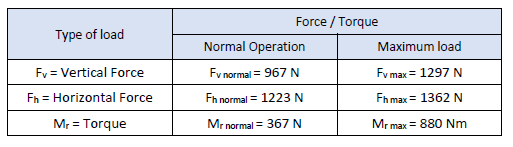
\includegraphics[scale = 0.95]{Loads}
\end{center}	
\end{figure}

Using steel A37 with the following specifications:
\begin{itemize}
	\item[--] Yield Strength: $\sigma_{y} = 235 MPa$
	\item[--] Ultimate Tensile Strength: $\sigma_{u} = 360 MPa$
\end{itemize}

The max allowable shear stress is:
$$ \tau_{all} = 0.3 (235) = 70.5 MPa $$
$$ \tau_{all} = 0.18 (360) = 64.8 MPa $$
\vspace{0.3 cm}
\newline The following table shows the different values of diameters available in market, along with the corresponding resulting shear stress:
\begin{figure}[H]
	\begin{center}
		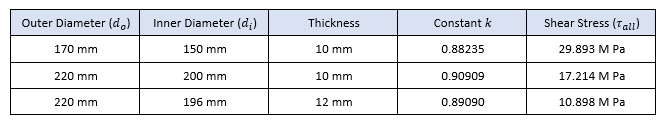
\includegraphics[scale = 0.95]{CalculationsResults}
	\end{center}	
\end{figure}

Thus, by comparing the previous values of resulting shear stress to the minimum value of the maximum allowable shear stress the material can withstand, 64.8 MPa, we find that any of the alternatives would be suitable for manufacturing the cylinder.

\bigskip

\subsubsection{Bolts’ diameters}
\begin{itemize}
	\item Lower flange
\end{itemize}

To get the diameters of the used bolts, we need to calculate the tension forces acting on them first. 
\begin{equation}
M_{b} = 2 F_{1} r_{1} + 2 F_{2} r_{2} = H F_{h}
\end{equation}
$$\frac{F_{1}}{r_{1}} = \frac{F_{2}}{r_{2}}$$
$$ F_{1} = F_{2} \frac{r_{1}}{r_{2}}$$
Substituting $F_{1}$ in equation (1.2), we get:
\begin{equation}
H F_{h} = 2 F_{2} (\frac{r_{1}^{2}}{r_{2}} + r_{2})
\end{equation}

Where $r_{1}$ and $r_{2}$ are the distances from one edge of the flange to the first pair of bolts, and the second pair respectively, as shown in figure below.
\begin{figure}[H]
\begin{center}
	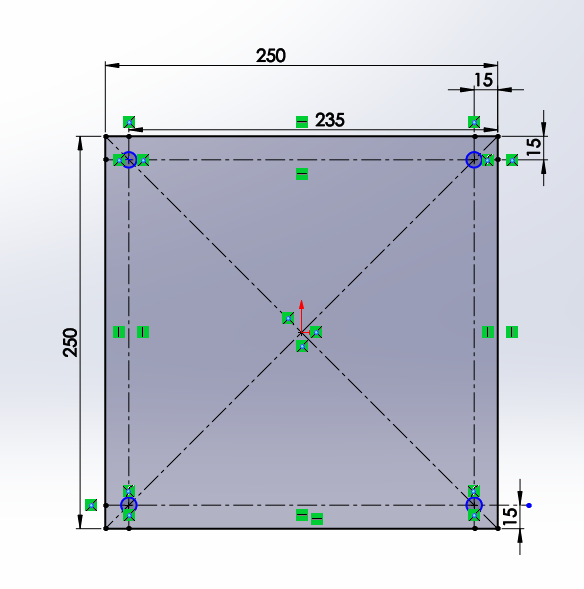
\includegraphics[scale=0.5]{R1R2}
	\caption{values of $r_{1}$ and $r_{2}$}
\end{center}	
\end{figure}

\textit{Notes:} 
\begin{itemize}	
\item[--]  The values of dimensions of the flanges and distances $r_{1}$ and $r_{2}$ are defined based on the assumption that the bolts used in the lower flange is 10 mm, until reasonable results are obtained using try and error.
\item[--] All dimensions mentioned in this chapter are measured in mm.
\end{itemize}



If the diameter of bolts holding the lower flange is 10 mm, and the area of the flanges is (250x250) $mm^{2}$, then the values of $r_{1}$, $r_{2}$ are 15 mm and 235 mm respectively, as shown in the figure below.
\newline Substituting the values of $M_{b}$, $r_{1}$, and $r_{2}$, we get:
$$ F_{2} = 2308.89 N $$
Repeating the previous steps by substituting $F_{2}$ with $F_{2}$, we get:
$$ F_{1} = 147.376 N $$

For safety purposes, the design of the bolts will be based on the larger tension force, $F_{2}$.
After obtaining the tensile forces on the bolts, the tensile strength ($\sigma_{t}$) should be calculated to check for safety:

\begin{equation}
\sigma_{t} = \frac{F_{t}}{\frac{\pi}{4} d^{2}}
\end{equation}

For 10 mm bolts diameter, and the previously calculated tensile force, we get:
$$ \sigma_{t} = \frac{2308.89}{\frac{\pi}{4} (0.01)^{2}} = 29.398 MPa $$ 

Taking in consideration a factor of safety, and checking for the maximum tensile strength the material can undergo before failing:
$$\sigma_{t} = \frac{\sigma_{y}}{F.S.} = \frac{235}{3} = 78.33  MPa$$
The resulting tensile stress is less than the maximum allowable tensile stress, hence, the previous design is safe.
\newline It was previously mentioned that we used commercial materials available in the market. The manufactured steel sheets are of thickness 15 mm, calculations need to be made to check for safety according the maximum shear and bearing stresses.
\newline The horizontal shear force exerted on the base will be acting on the bolts as well, however, it is negligibly small because it’s mostly eliminated by the existence of friction between the two steel flanges it holds. Moreover, the moment resulting from tightening the bolts produces an axial force eliminating the axial load acting on the base.

\begin{figure}[H]
	\begin{minipage}{0.5\textwidth}	
		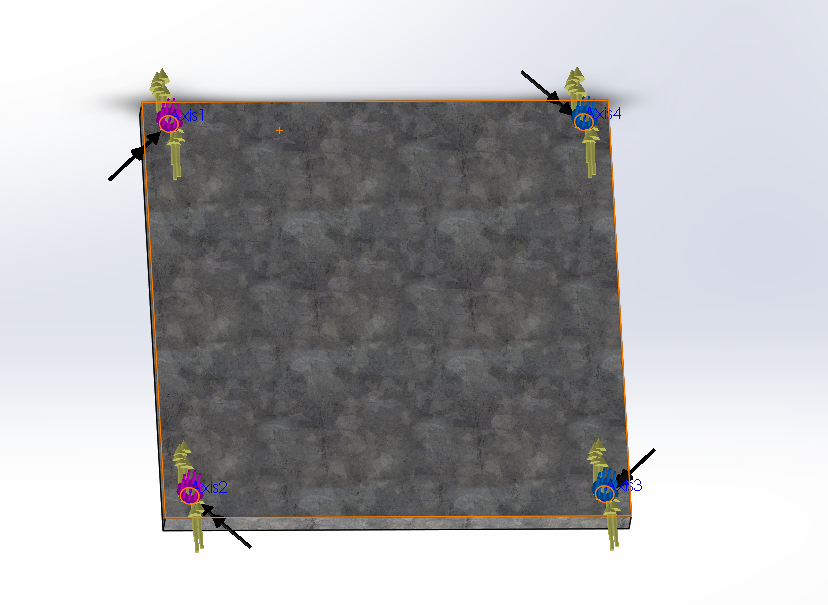
\includegraphics[scale=0.35]{CombinedForces1}
	\end{minipage} \hfill
	\begin{minipage}{0.6\textwidth}
		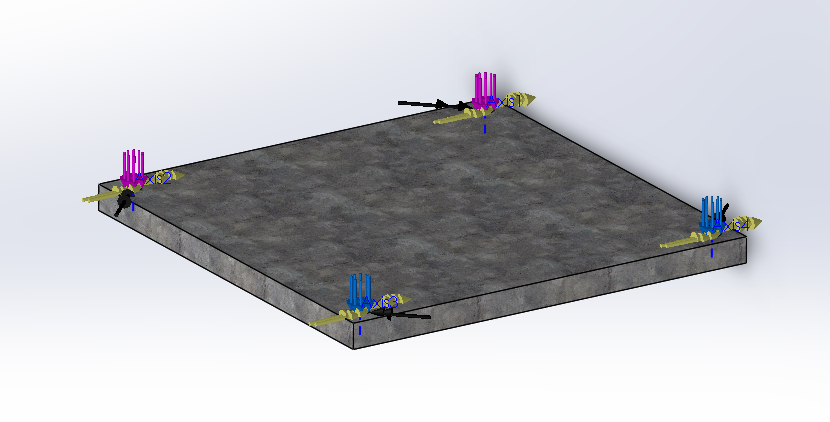
\includegraphics[scale=0.5]{CombinedForces2}
	\end{minipage}
	\begin{center}
		\caption{Forces acting on bolts. Black arrows: $F_{tr}$ , purple: $F_{a}$, green: $F_{h}$ }
	\end{center}
\end{figure}

\begin{equation}
F_{total} = \sqrt{(\frac{F_{h}}{4})^{2} + (F_{tr})^{2} + 2 F_{tr} F_{h} cos \theta}
\end{equation}

\begin{equation}
F_{tr} = \frac{M_{t}}{4 R}
\end{equation}

Where R,which  is the radius of perimeter, has a value of 176.78 mm  as shown in figure below.

\begin{figure}[H]
	\begin{center}
		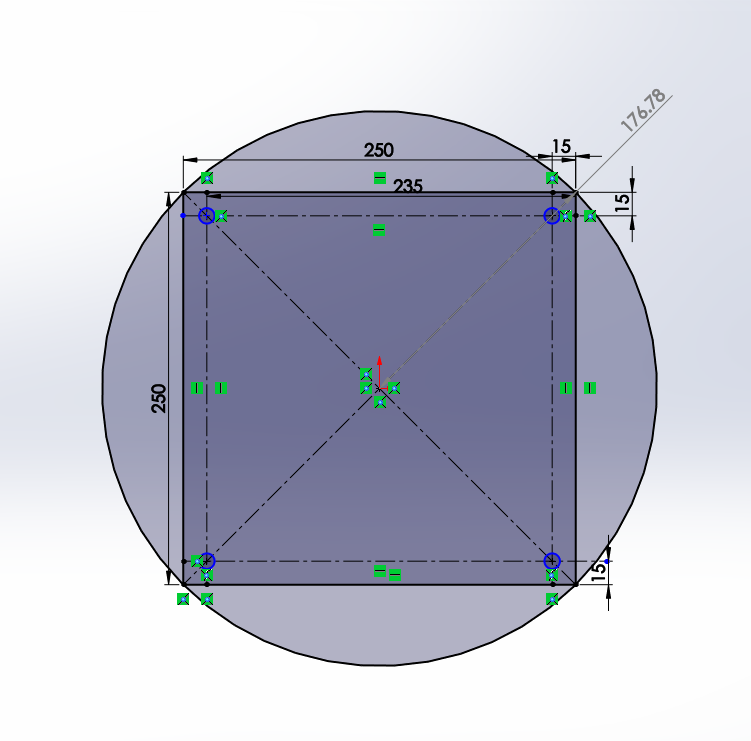
\includegraphics[scale = 0.3]{R}
		\caption{value of R}
	\end{center}
\end{figure}

$$ F_{tr} = \frac{880}{4 (0.1768)} $$
$$ F_{total} = \sqrt{(\frac{1362}{4})^{2} + (\frac{880}{4 (0.1768)})^{2} + (2\frac{1362(880)}{4(4)0.1768} cos 45)} = 1504.5 N $$

Checking for safety in terms of the bearing stress:
\begin{equation}
\sigma_{br} = \frac{F_{total}}{d_{b} t} = \frac{1504.5}{0.01(0.015)} = 10.03MPa
\end{equation}

By comparison to the maximum allowable bearing stress, we find that both of the predetermined bolt diameter (10 mm), and the flanges thickness are verified to be safe and suitable, as following:

\begin{equation}
\sigma_{br} = 1.2 \frac{\sigma_{y}}{F.S.} = \frac{1.2(235)}{3} = 94 MPa
\end{equation}

Checking on the maximum shear stress exerted on the bolts by the combined forces, we get:

\begin{equation}
\tau = \frac{F_{total}}{\frac{\pi}{4} (d_{b})^{2}} = \frac{1504.5}{\frac{\pi}{4} (0.01)^{2}} = 19.156 MPa
\end{equation}
Comparing it to the maximum shear stress the bolts can stand which is 64.8 MPa since it's made of the steel-37 as well, we can conclude that this is a safe design in terms of the bolts diameters, flanges dimensions, and cylinder diameters.

\bigskip

\subsubsection{Upper Flange}
The upper flange holds the robot base motor, using the bolts provided with the robot. The flange was designed to have an area of (230x230) $mm^{2}$, with the locations of 4 bolts holding the robot taken from its base.

\bigskip

\subsubsection{Ribs}
The ribs are made of the same sheet of which the flanges are made of, with a thickness of the ribs is 10 mm. 
\newline There isn’t an exact way of calculating the height and width of the triangular ribs. After discussing the matter with several machine design doctors, we concluded that the ribs’ width should cover the length from the cylinder surface to the edge of flange, resulting in a width of 55 mm, while the height is 100 mm.


\newpage

\subsection{Base Manufacturing \& Installation }

\subsubsection{Manufacturing}

Several materials can be used to manufacture the body of the base, such as AISI 1010 \& AISI 1010 carbon steel, SAE 304 stainless steel, etc., all of which the mechanical properties are predefined. However, the available material in the market was steel 37, which has the following mechanical specifications:

\begin{itemize}
	\item[--] Yield Strength: $\sigma_{y} = 235 MPa$
	\item[--] Ultimate Tensile Strength: $\sigma_{u} = 360 MPa$
\end{itemize}


The calculations performed on this material are proven to be safe and suitable to our designed base geometry. 
\vspace{0.2 cm}
\newline The squared, upper and lower flanges are made of a 15mm thick steel-37 sheet, and holes were drilled in the designated locations shown in the sketches below. The flanges are then welded to the cylindrical body of the base. It’s worth mentioning that the dimensions of the manufactured base are larger than those calculated, this is due to different manufacturing and safety purposes, the final dimensions manufactured are illustrated below.
\begin{figure}[H]
\begin{center}
	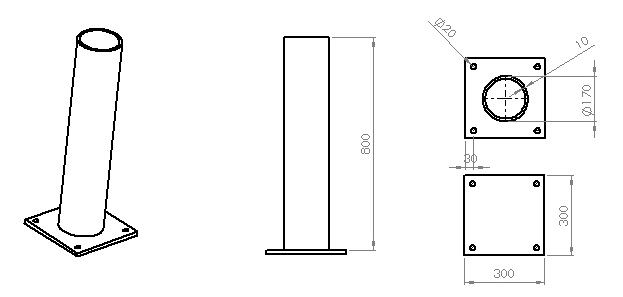
\includegraphics[scale=0.5]{BaseDim}
	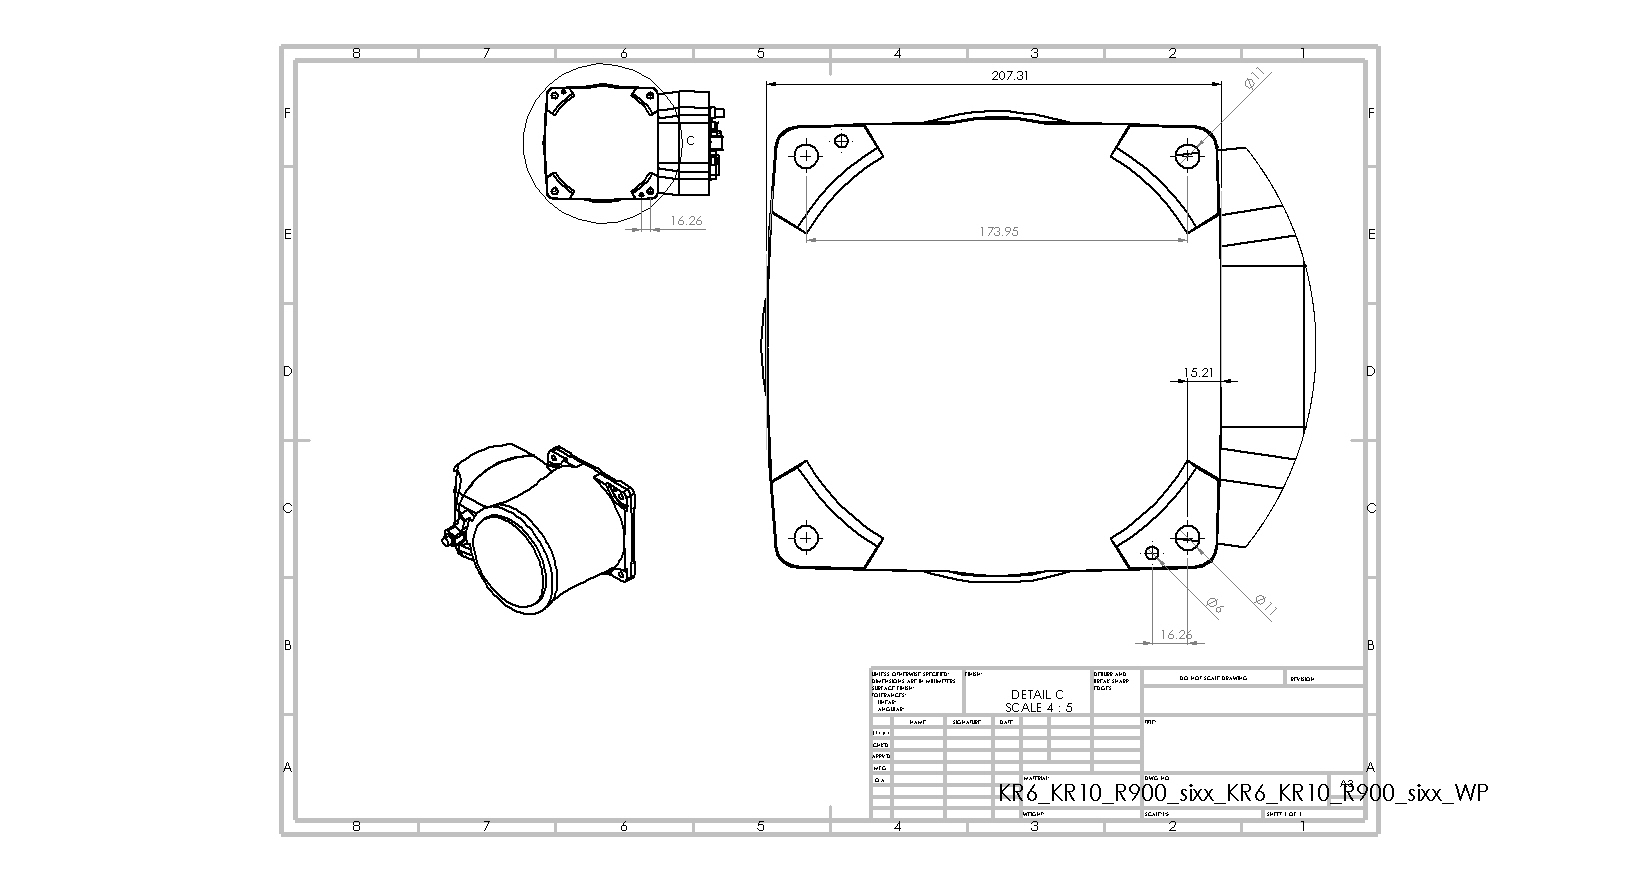
\includegraphics[scale=0.5]{BaseDim2}
	\caption{Final dimensions manufactured base}
\end{center}
\end{figure}


For the ribs to be welded, the base needs to be cleaned of any accumulated rust, it is then taken to undergo different machining steps, using a lathe machine. Next, it is painted in black to match the robot colors.
\newline \figurename{1.4} illustrates different stages of manufacturing.

\begin{figure}[H]
\begin{center}
	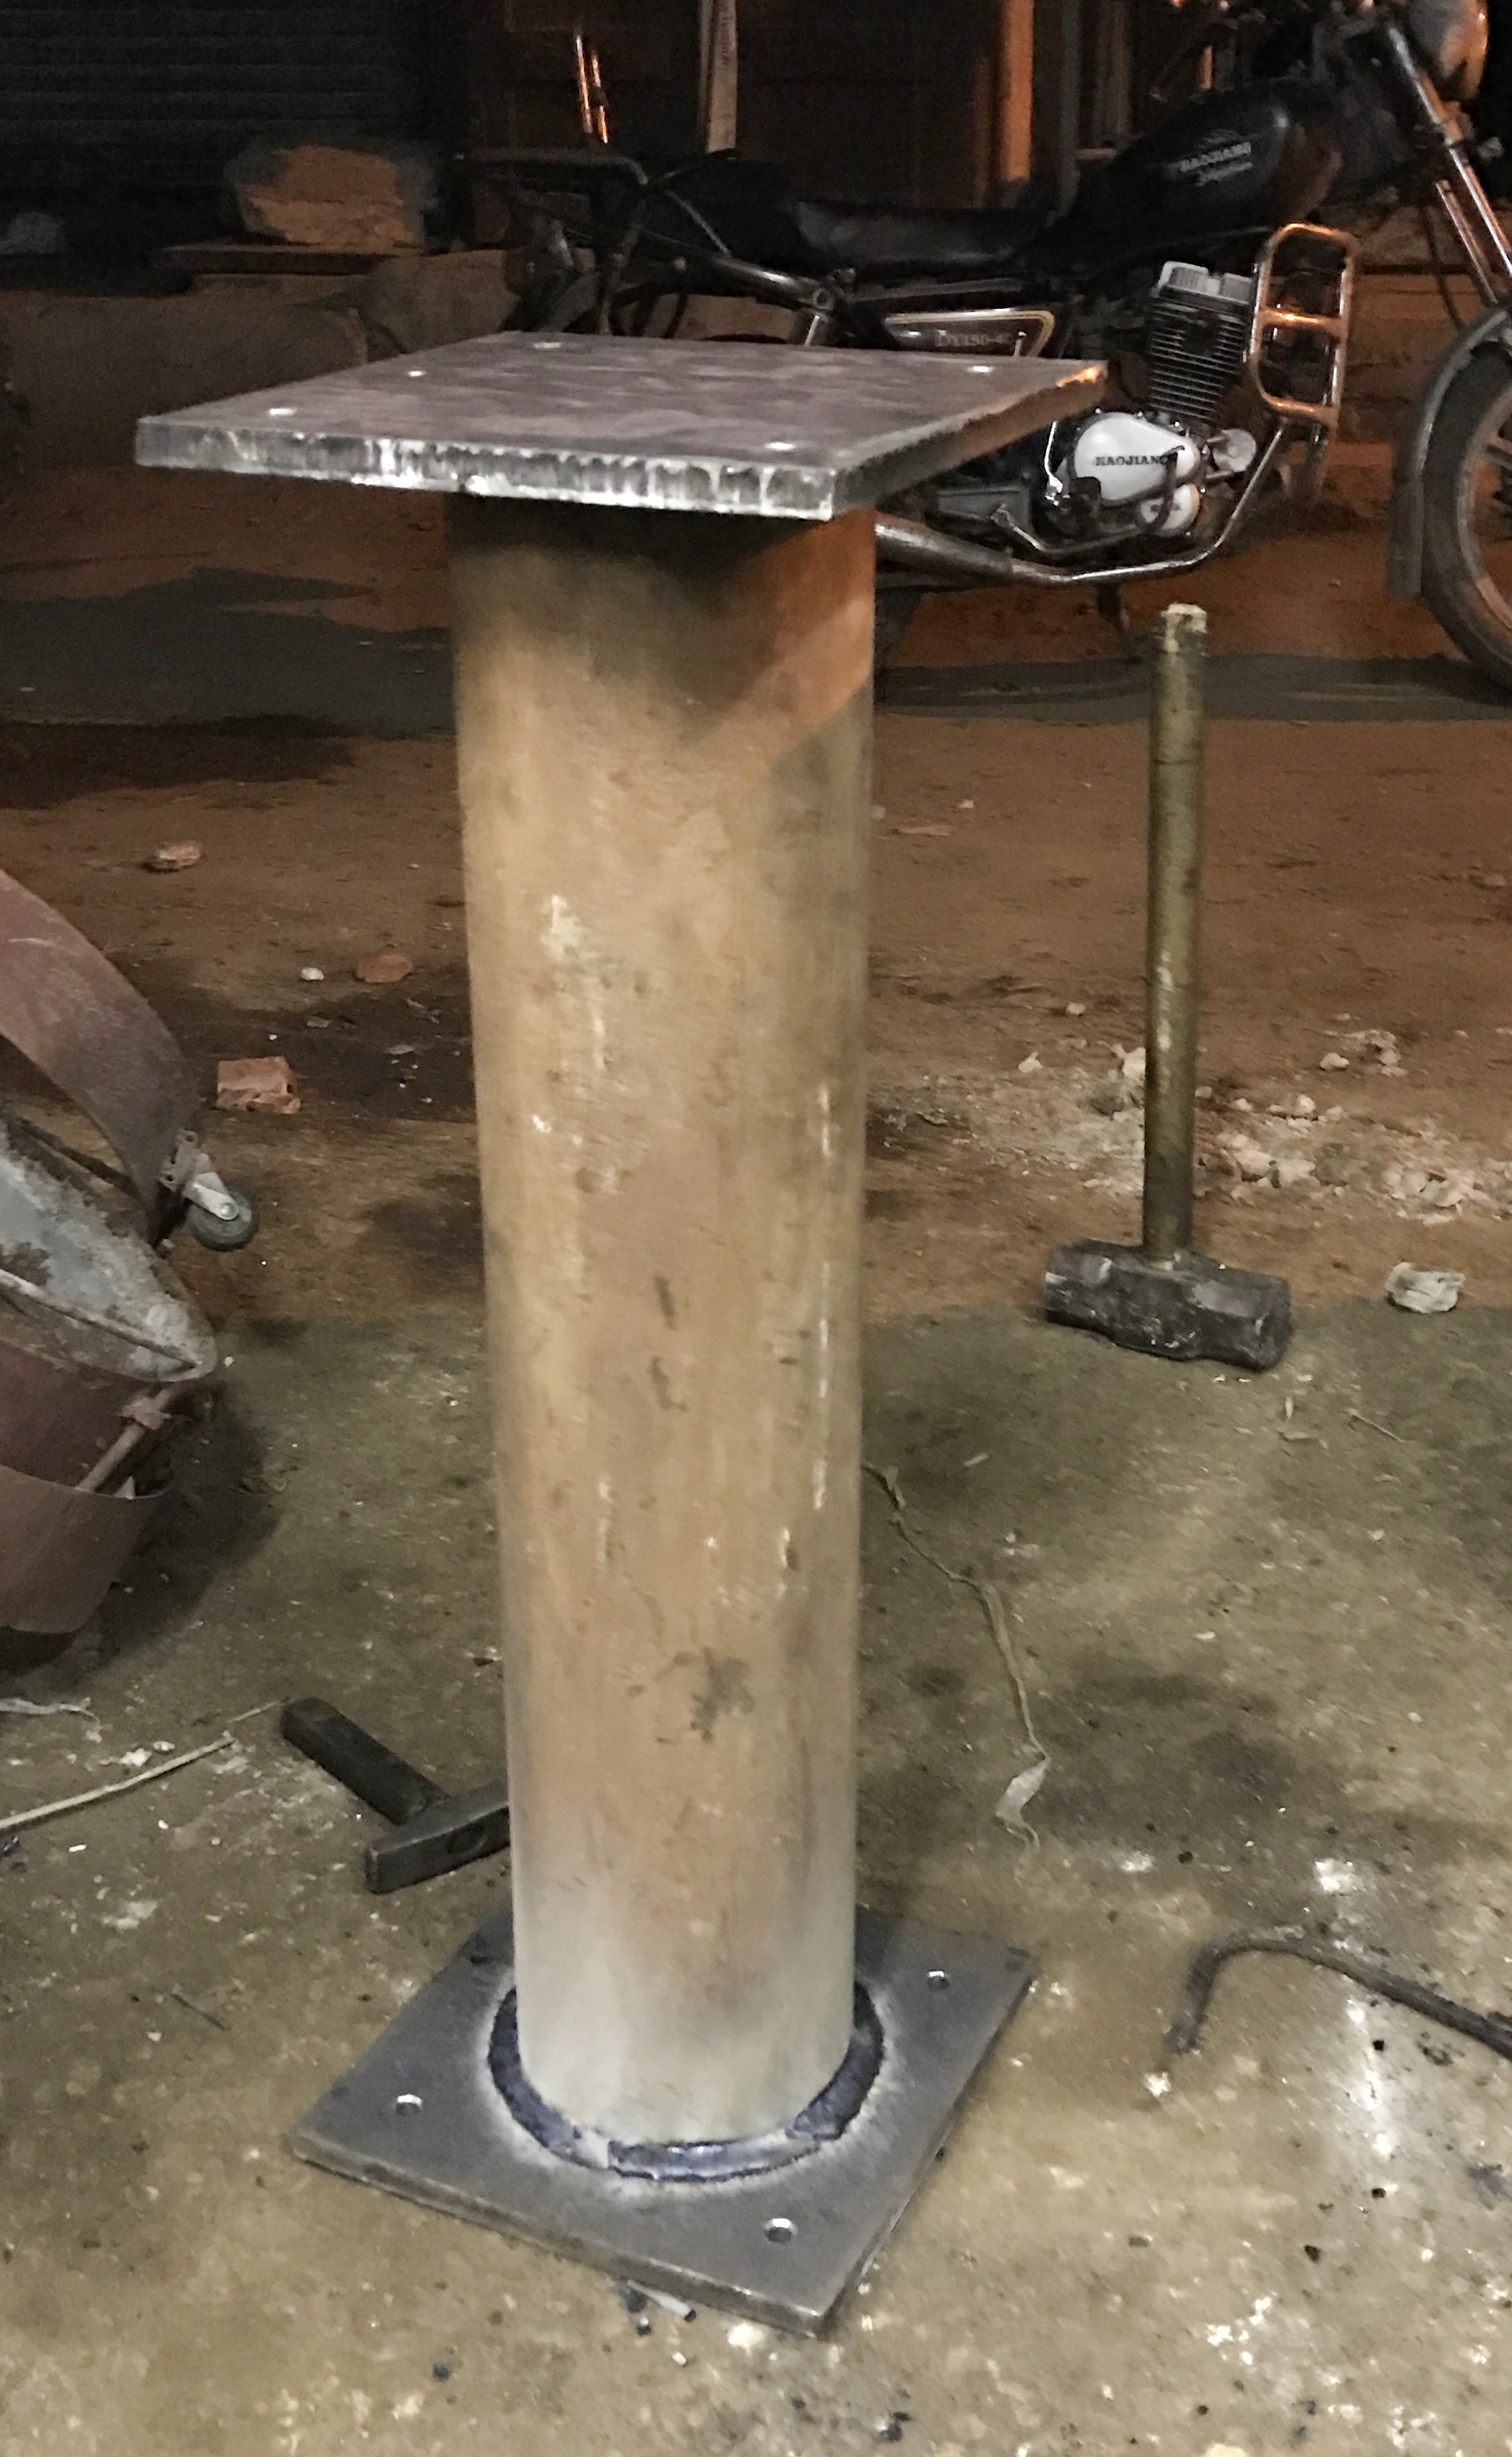
\includegraphics[scale=0.055]{WeldedFlanges}
	\includegraphics[scale=0.04]{Lathe}
	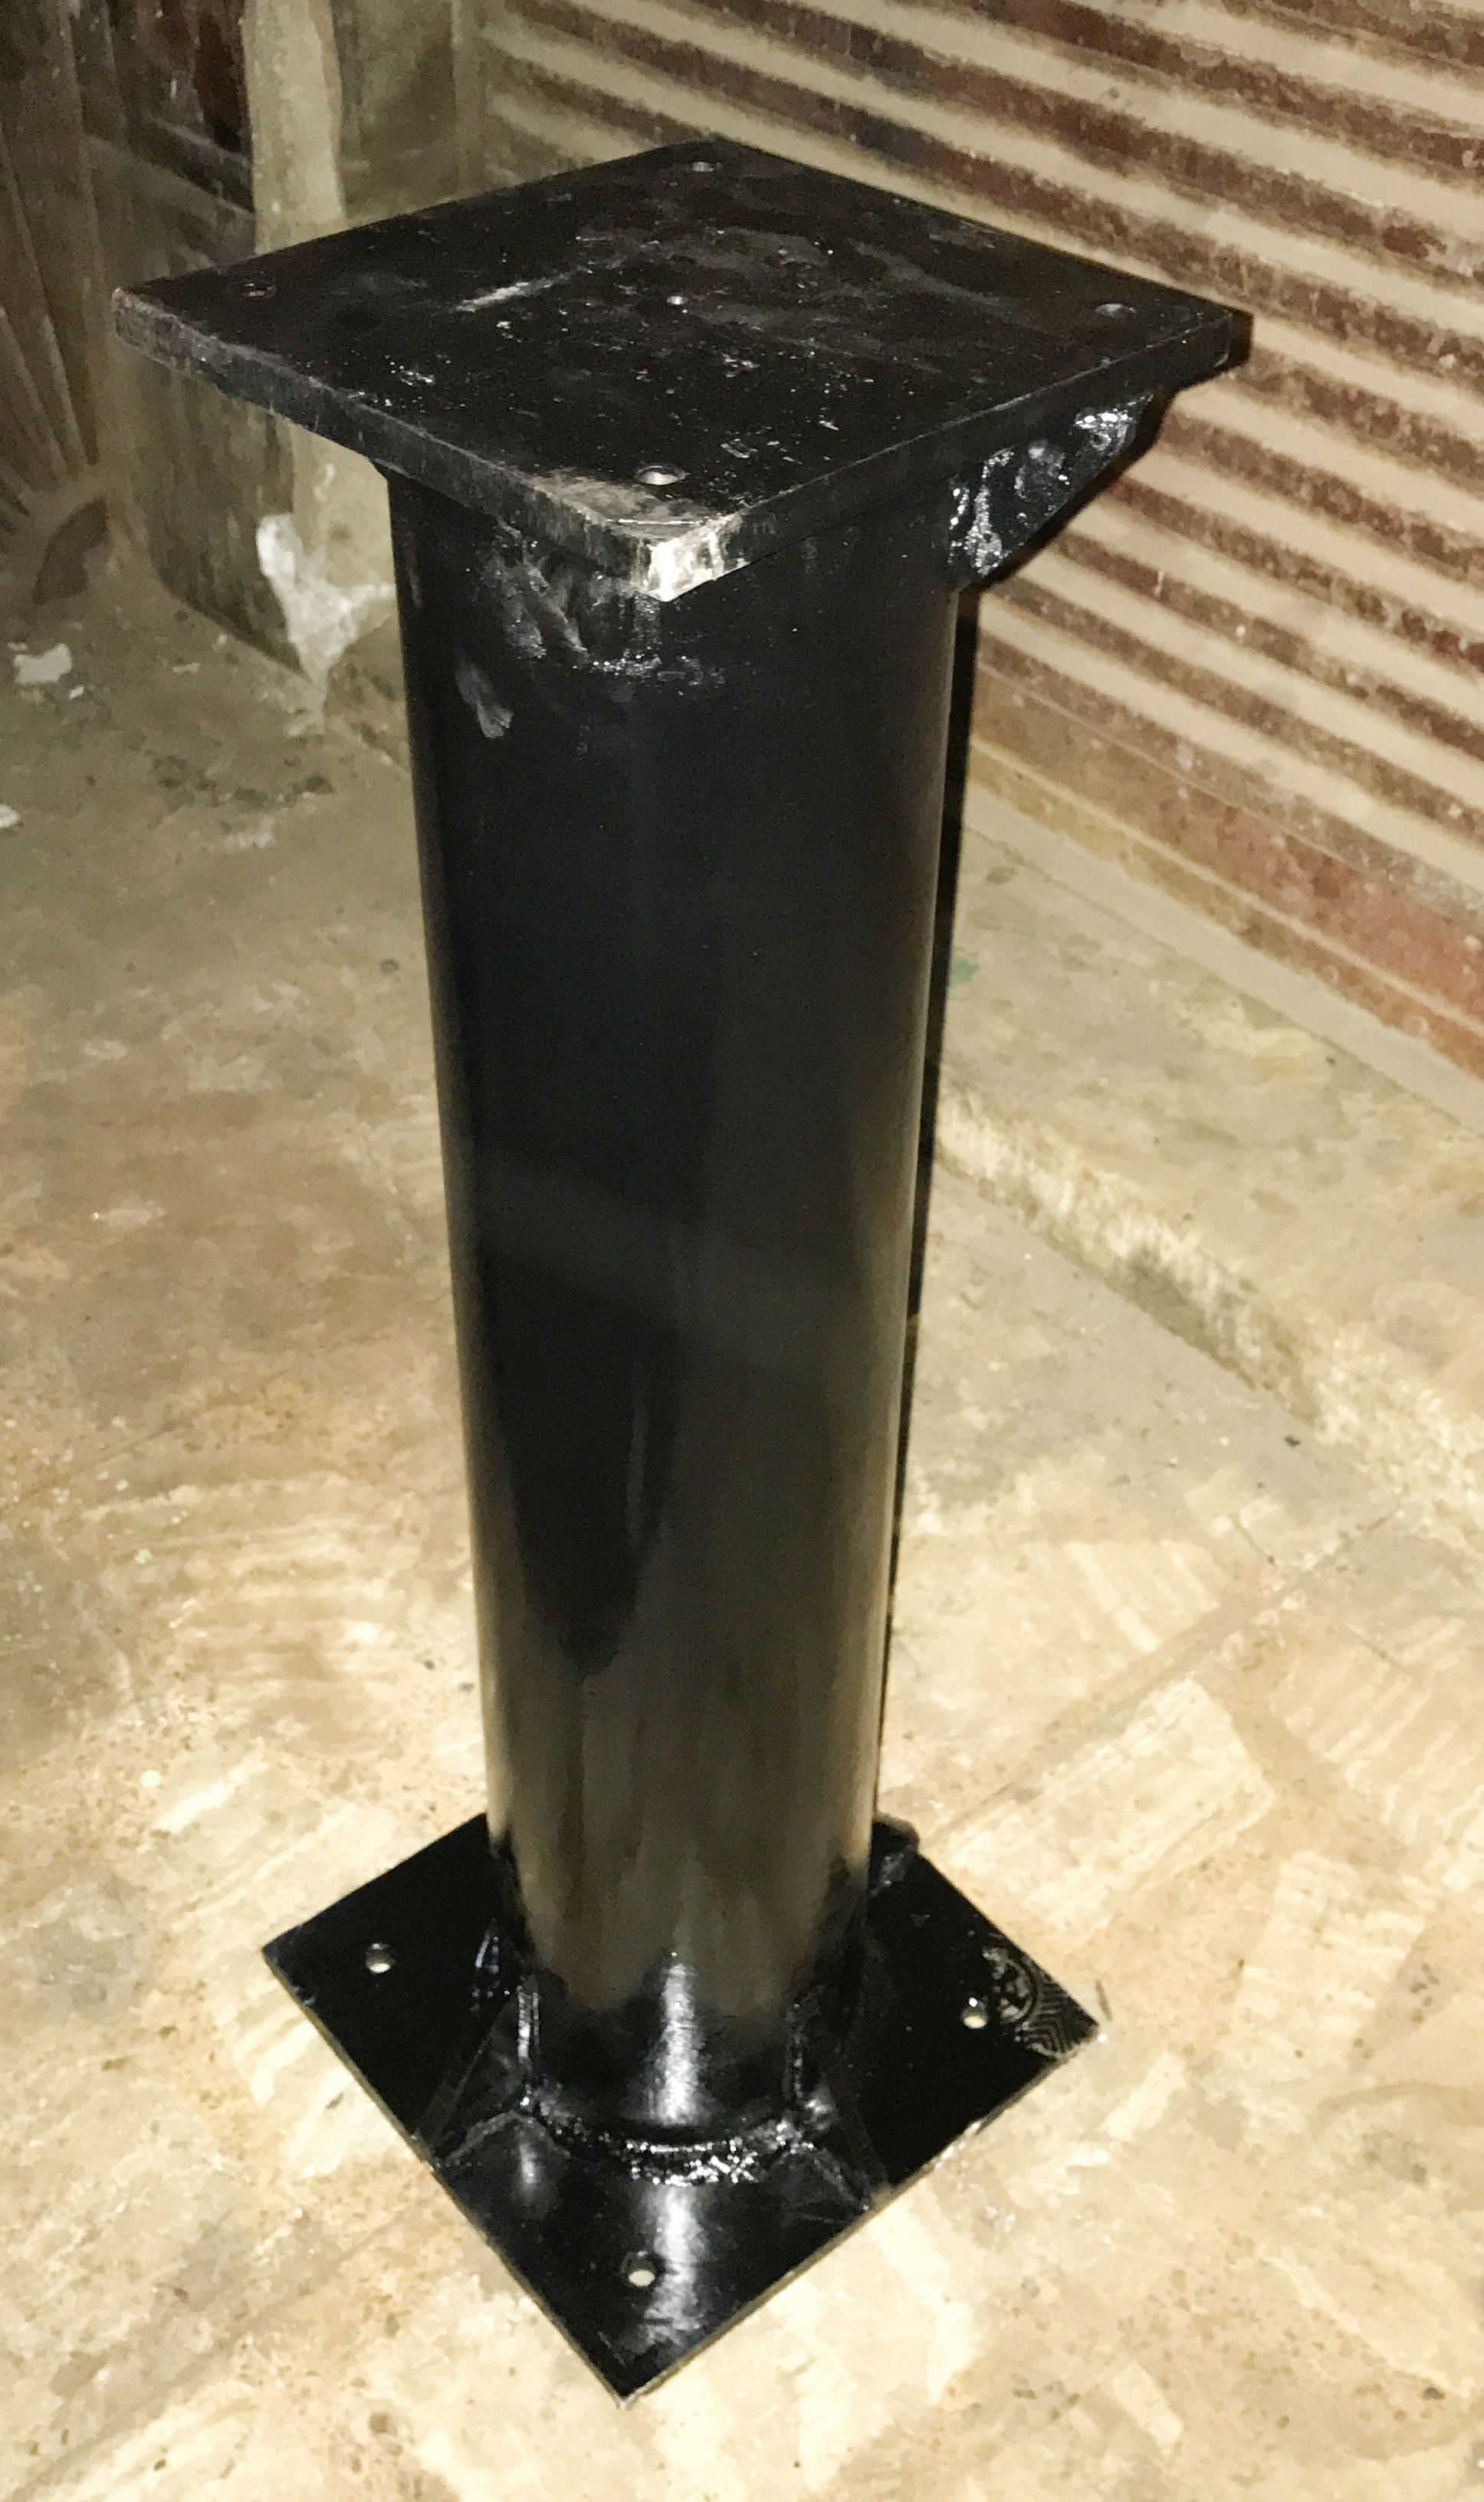
\includegraphics[scale=0.049]{PaintedBase}
	\caption{Manufacturing and Machining of the base}
\end{center}
\end{figure}

\subsubsection{Installation}

The following steps clarifies the process of installing the robot base:
\begin{enumerate}
	\item The exact location of the base is chosen according to the safe operating range of the robot, mentioned in the KR AGILUS sixx specification manual.
	\item Remove the ceramic plate. The number of plates removed depends on the area of the base and the ceramic plate itself, in our case, only one plate was removed.
	\item Scrape the sand and cement layers beneath the ceramic until you reach the concrete, it can be recognized when a layer of gravels appears.
	\item Drill the holes, in which the dowel rods will be placed, in the predesigned positions in the concrete. For this design, seven holes were drilled, however, the number of dowels depends on the design.
	\item Make a mixture of sand, gravels, cement and anabond adhesive agent to mold a new concrete layer, and keep mixing until it’s consistent.
	\item Pour in the concrete mixture on top of the pre-existent one, while the dowels are placed, and wait for 2 days to ensure that it’s completely solidified.
	\item Remove the dowels and start screwing the bolts.
    \item Start mounting the first flange. Use a bubble level to check if it lies in a perfectly horizontal position, if not, you must scrape the newly molded concrete layer until it’s even. 
	\textit{\newline Note: Even out the newly molded concrete once it dries, this would help you to avoid such issues in further steps.}
	\item Mount the base, then move the robot carefully until it’s placed on it in the right orientation.
\end{enumerate}

\figurename{1.5} illustrates different stages of the previously explained installation process.

\begin{figure}[H]
\begin{center}
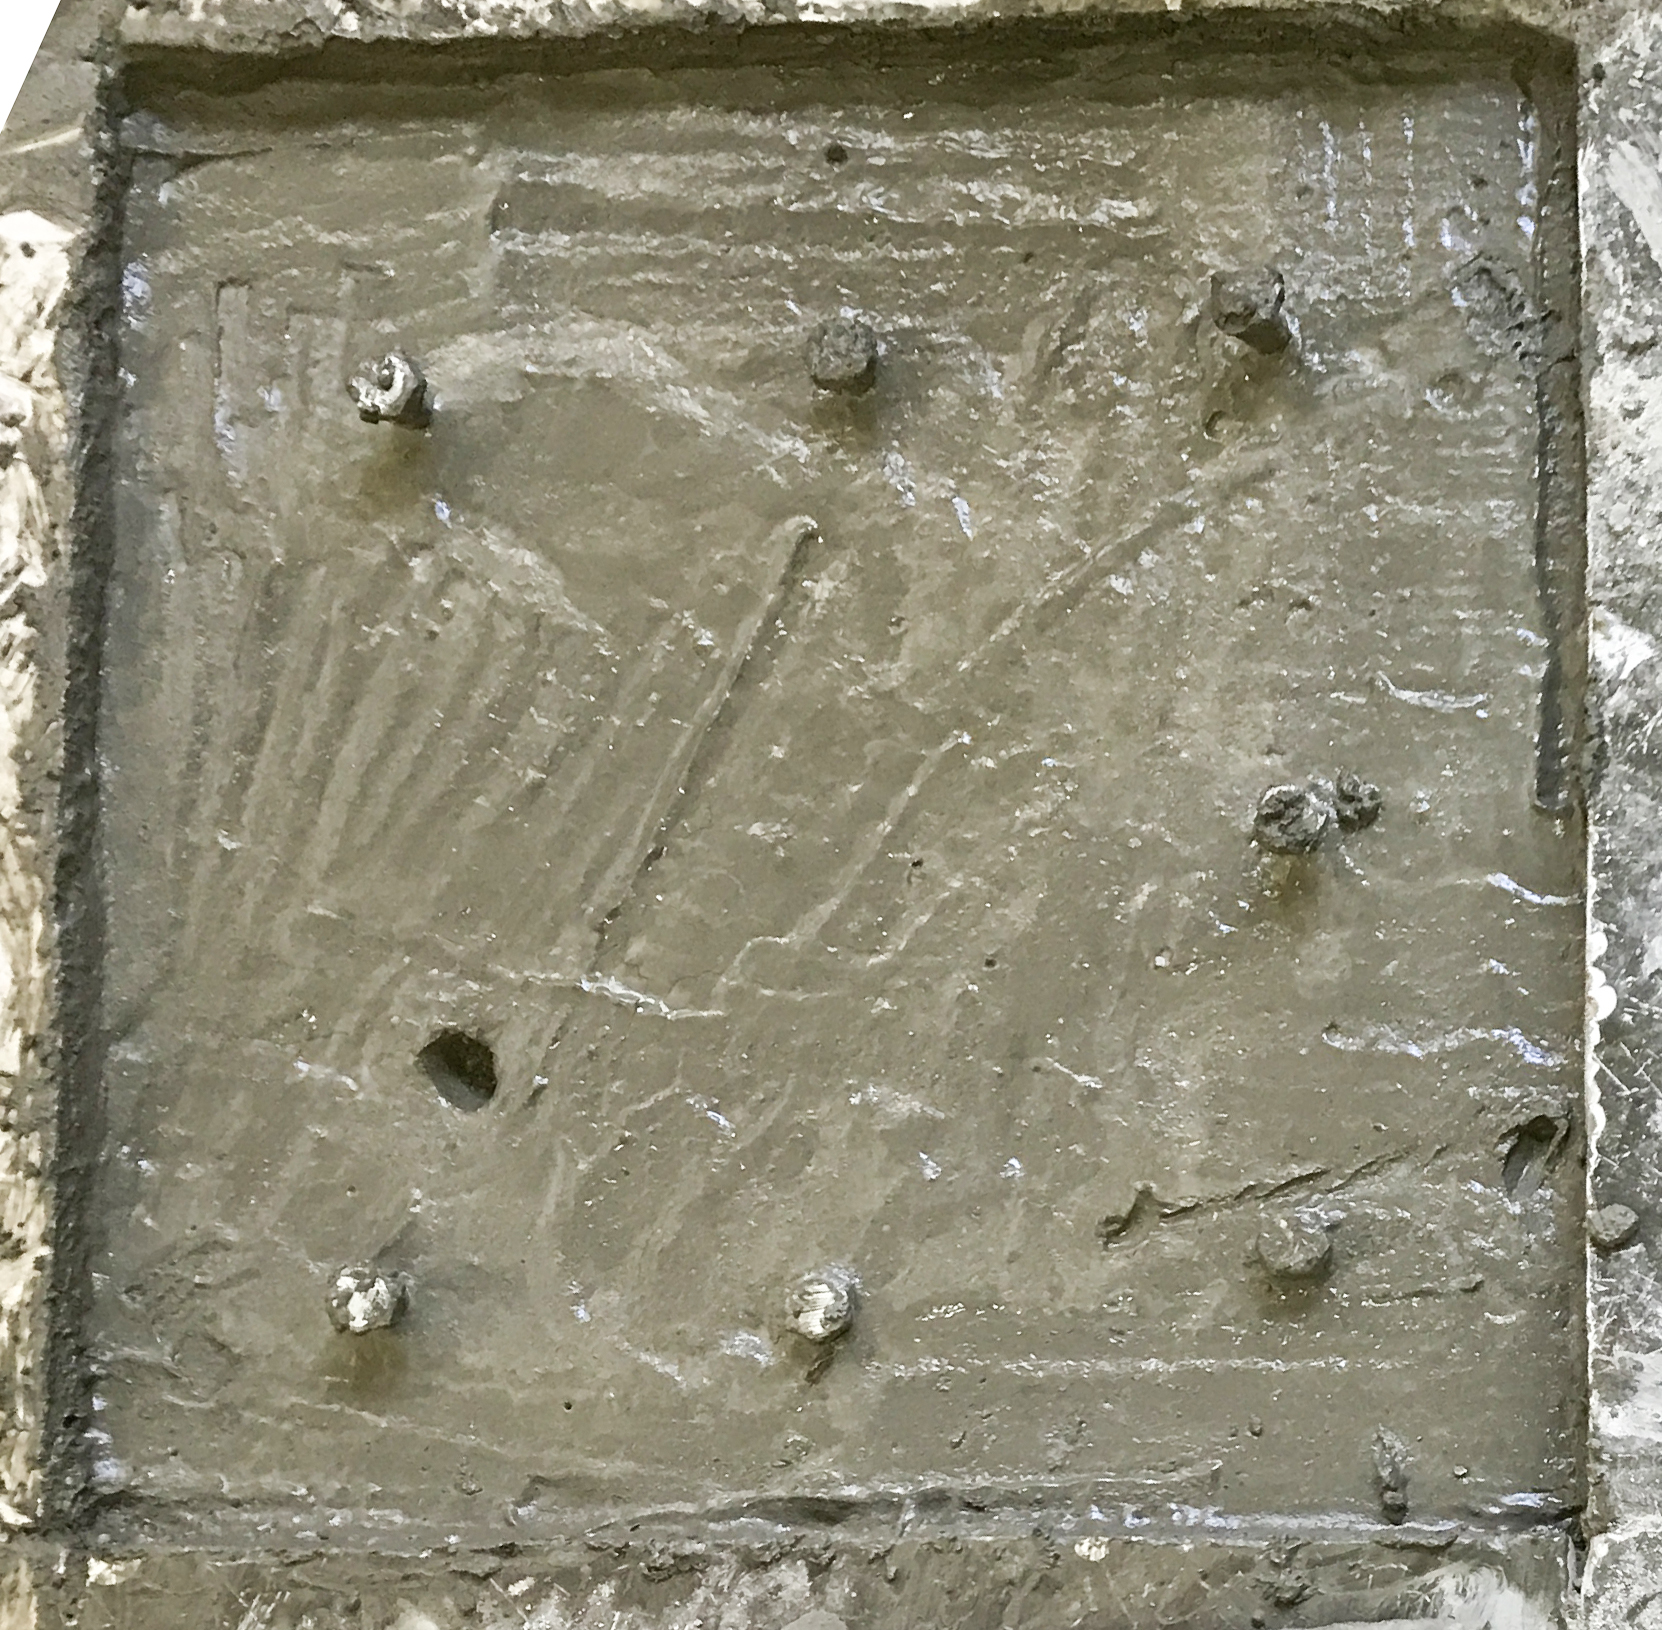
\includegraphics[scale=0.098]{MoldedConcrete}	
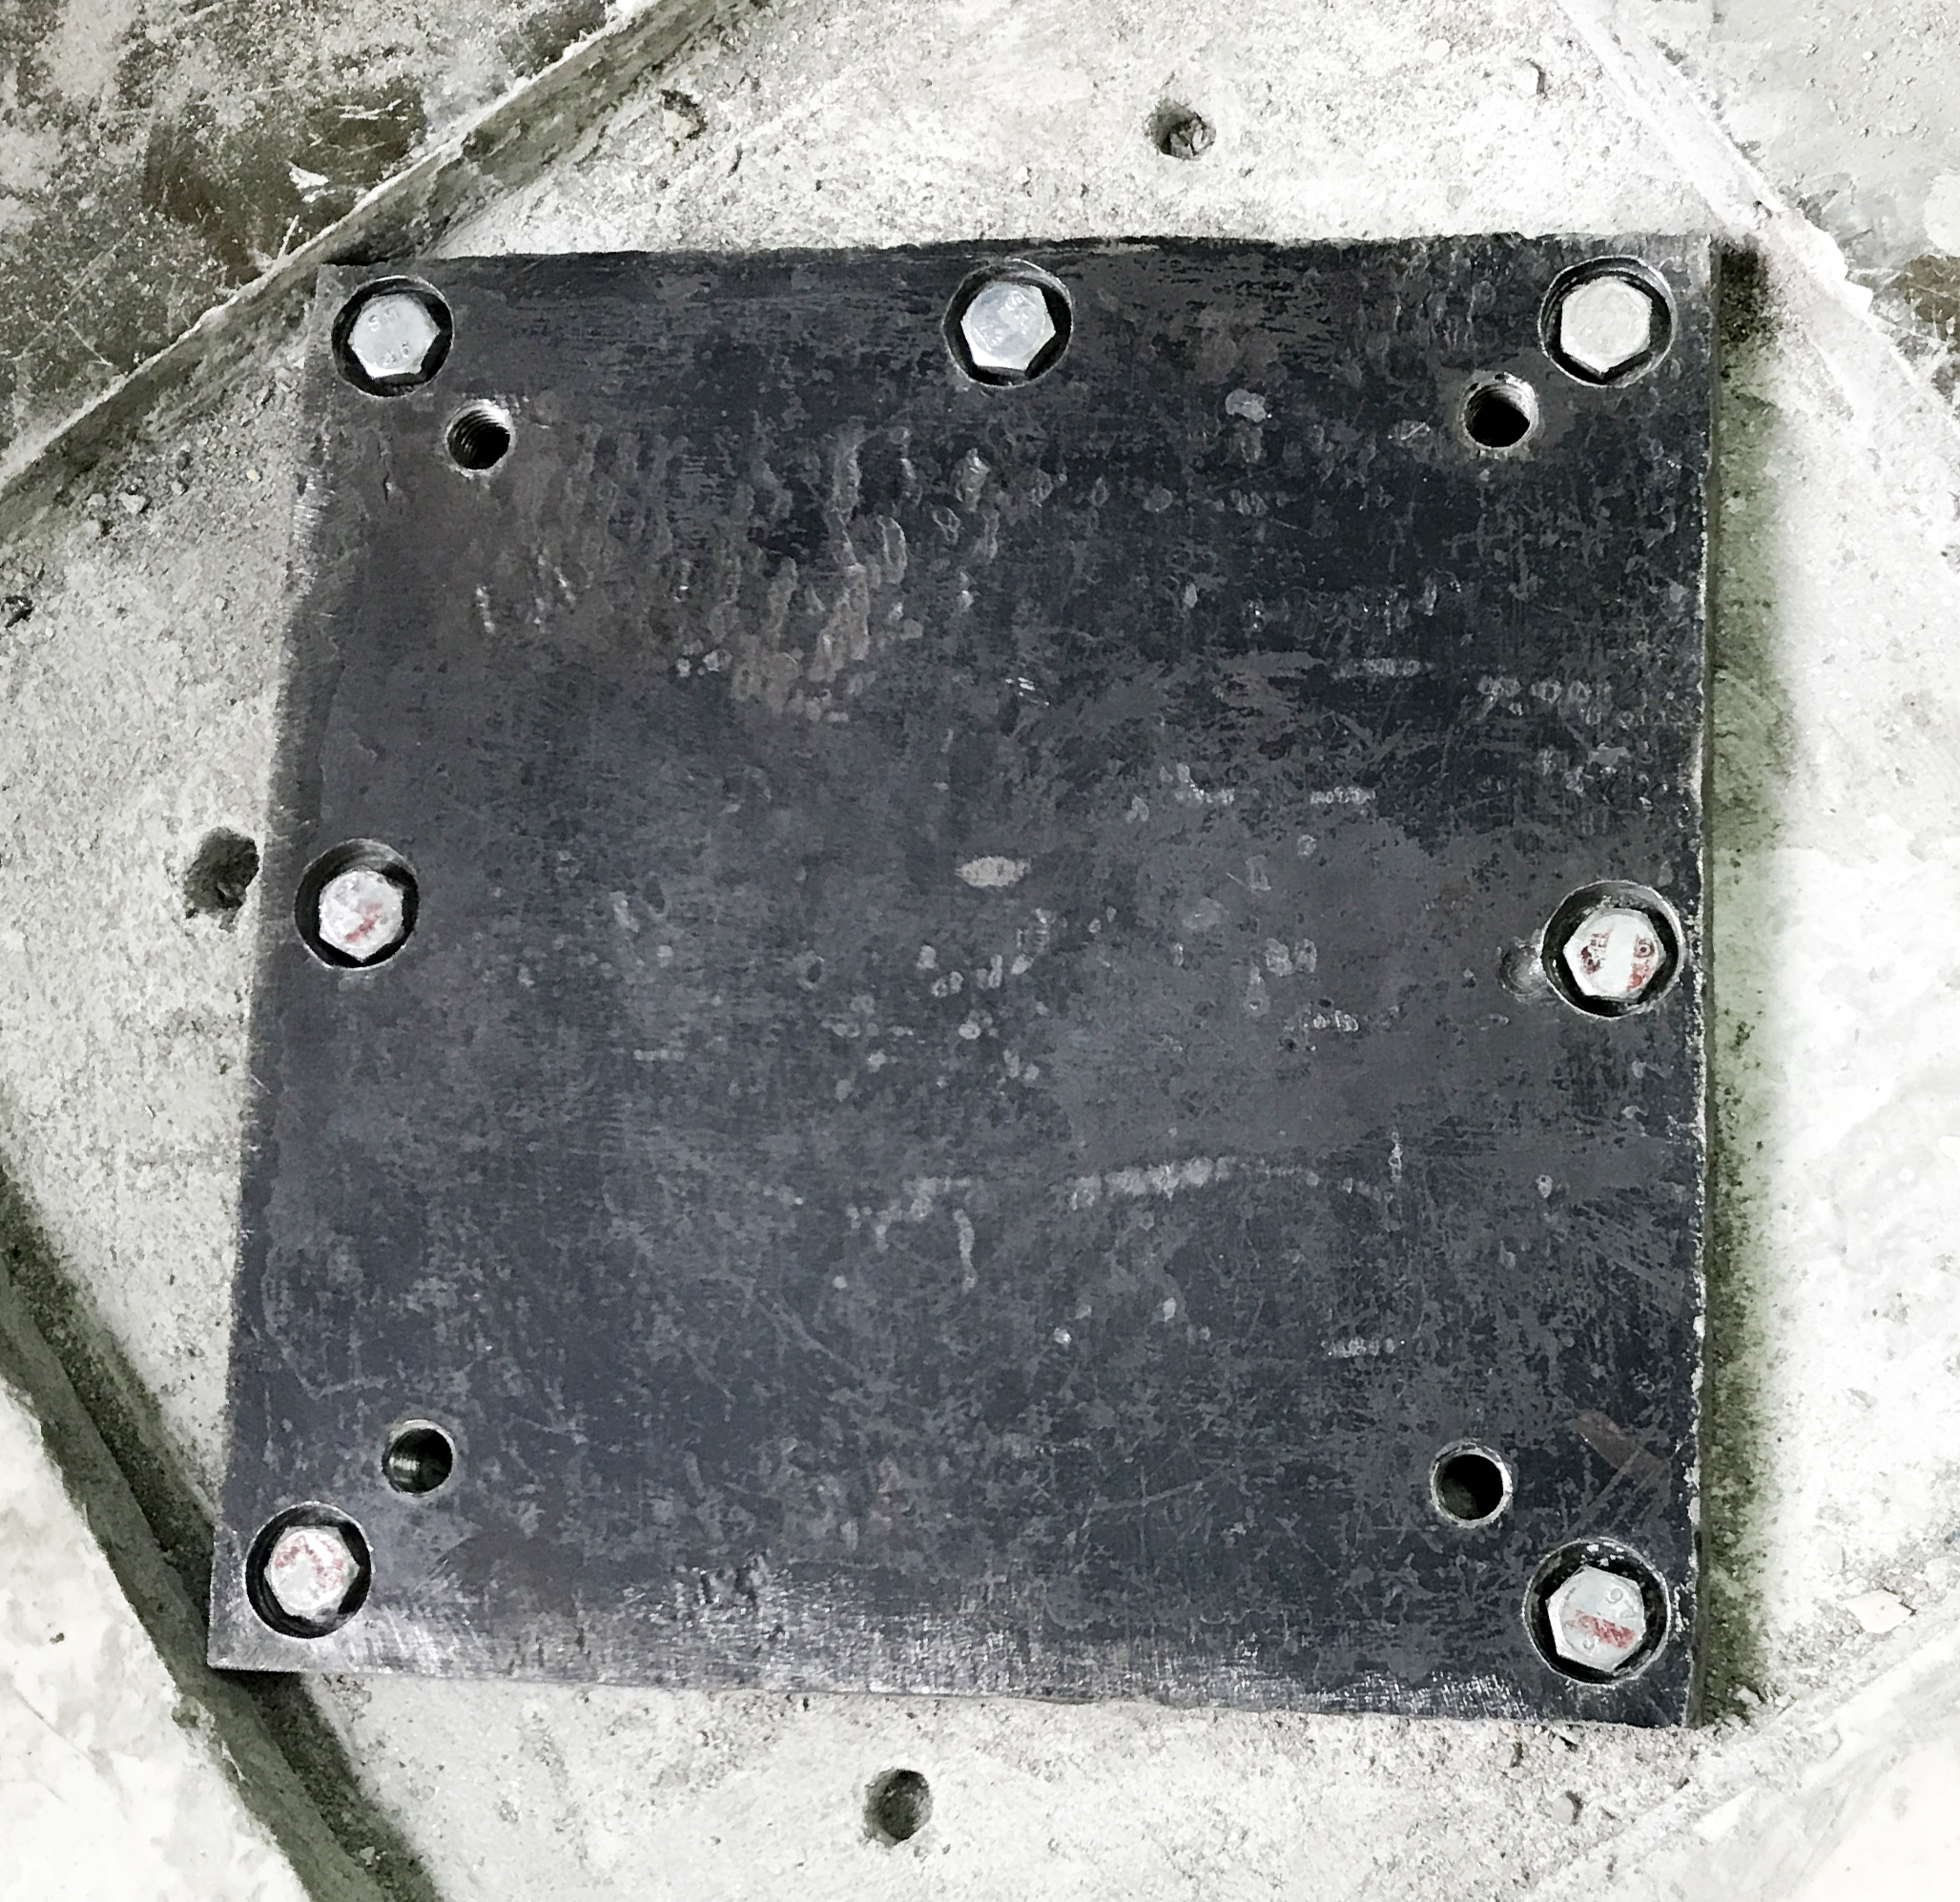
\includegraphics[scale=0.08]{FirstFlange}
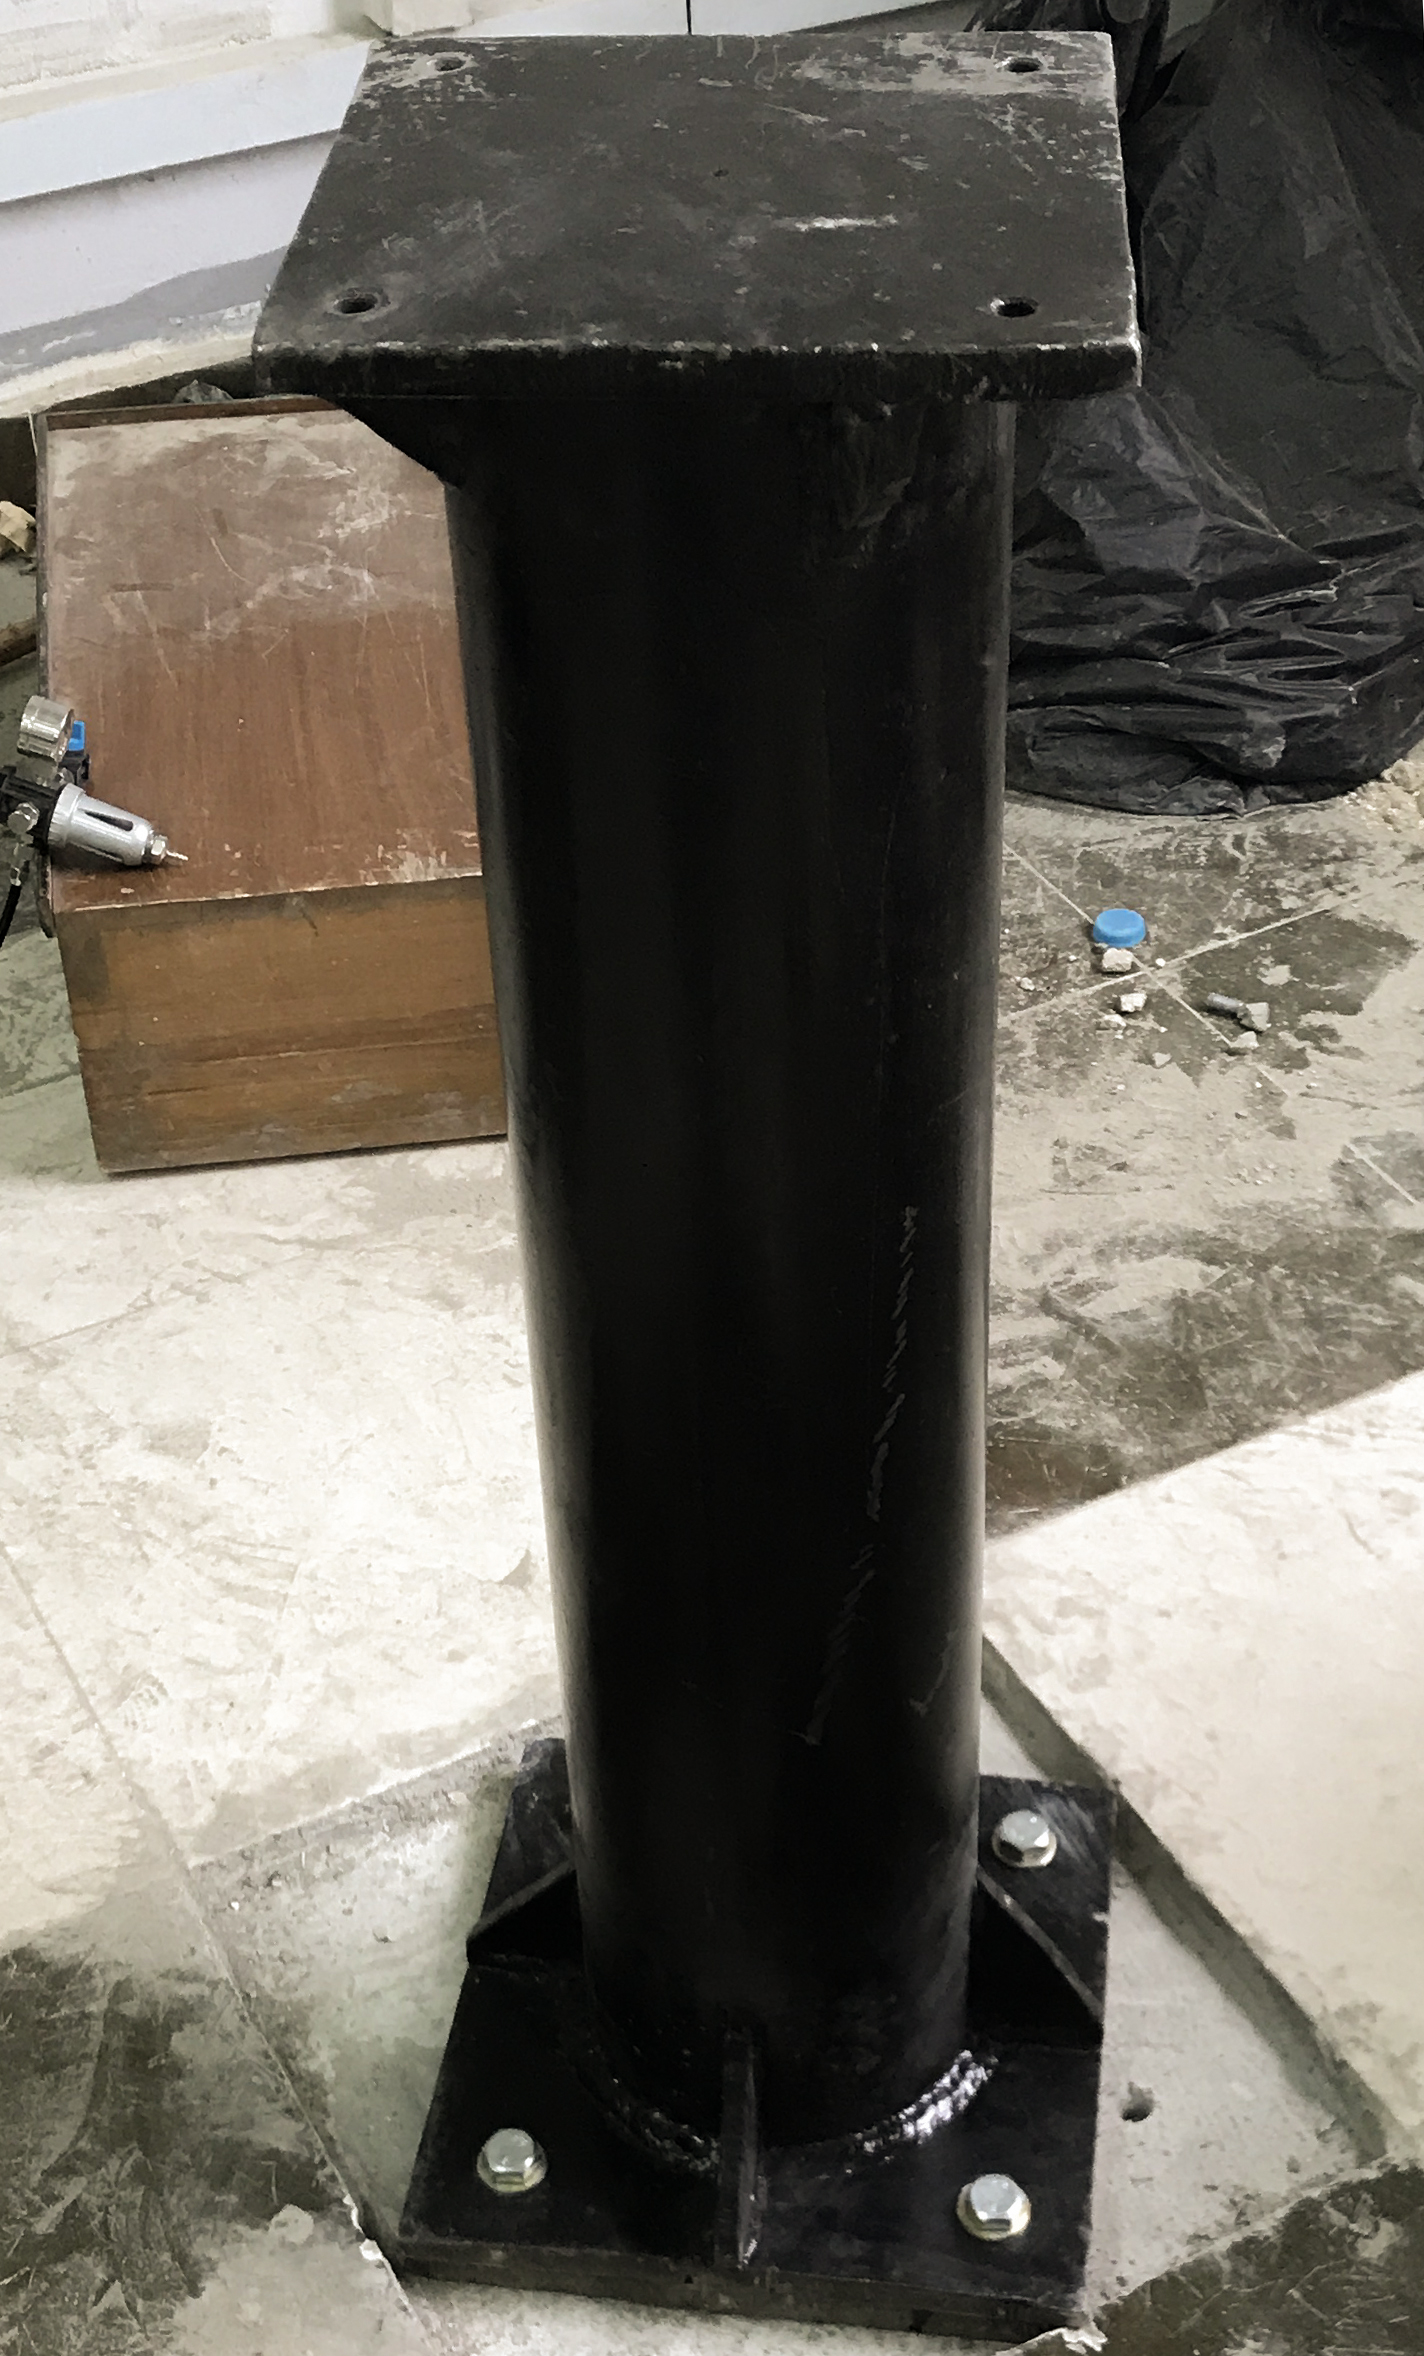
\includegraphics[scale=0.08]{MountedBase}
\caption{Base Installation}
\end{center}
\end{figure}



\newpage
\subsubsection{CAD Analysis Performed on Base}
For the purpose of our study, SolidWorks was used as a CAD software, as it contains solid modeling, motion studies, Simulation PhotoView 360, e-drawing and many other features that were used to obtain a complete CAD model for KR6 r900 sixx KUKA arm. 
\newline SolidWorks simulation is used to make a stress and strain analysis on designed base model to have a verification on the calculated dimensions of the base before starting fabricating it. Static study is used to perform this analysis as we use maximum loads acting on foundation base 


\begin{figure}[H]
	\centering
	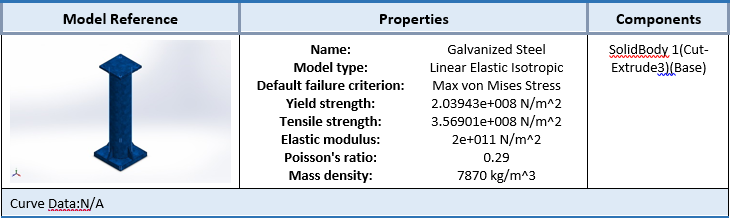
\includegraphics[scale=0.7]{material_properties}
	\caption{Solidworks definition for the material mechanical properties.}
\end{figure}



\begin{figure}[H]
	
	\centering
	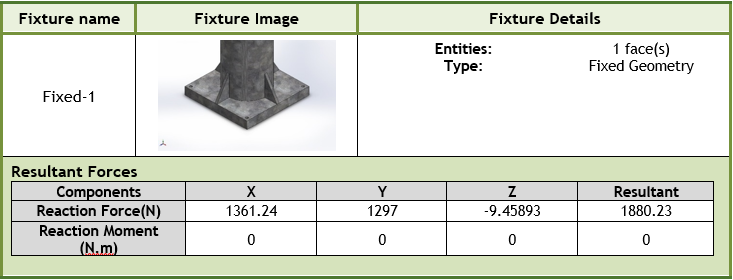
\includegraphics[scale=0.7]{load_And_fixture}
	\caption{Solidworks model reactions acting on the flange in x, y, and z.} 
\end{figure}


\begin{figure}[H]
	\centering
	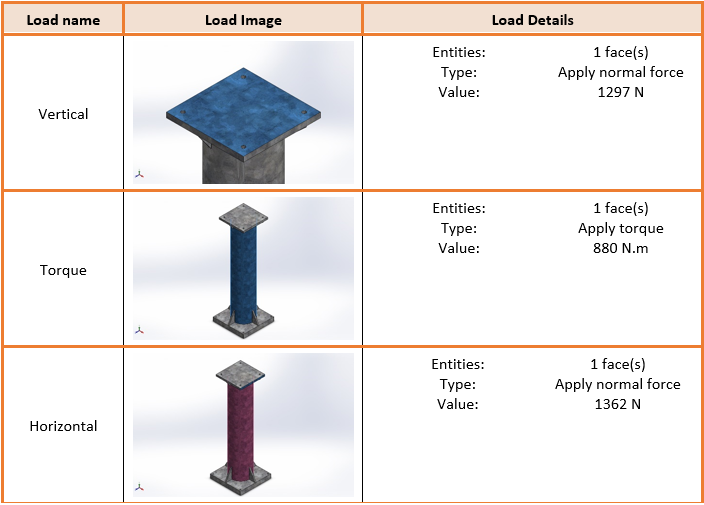
\includegraphics[scale=0.7]{load}
	\caption{Solidworks representation for different loads acting on the whole cylinder} 
\end{figure}

\begin{figure}[H]
	\centering
	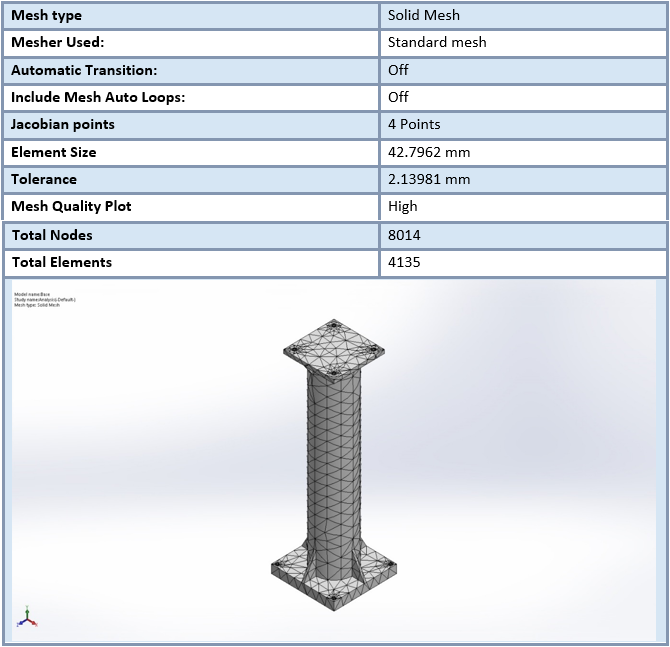
\includegraphics[scale=0.6]{mesh3}
	\caption{Mesh information obtained from Solidworks} 
\end{figure}

\begin{figure}[H]
	\centering
	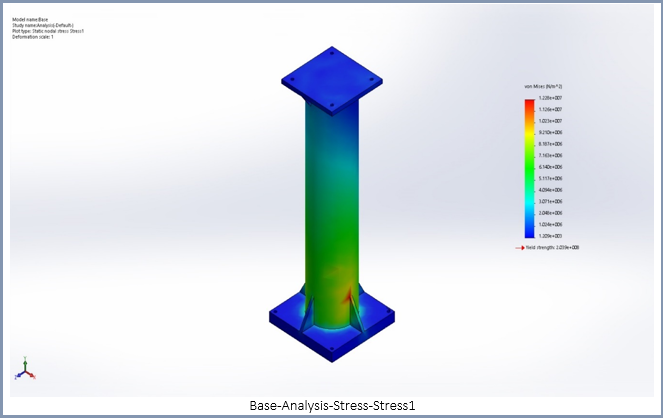
\includegraphics[scale=0.45]{zstress}
	\caption{Solidworks representation for stresses acting on the base.} 
\end{figure}
\begin{center}
	The maximum stress is 10.34 $N$/$m^{2}$ and the minimum stress is 6.8 $N$/$m^{2}$ .
\end{center}

\begin{figure}[H]
	\centering
	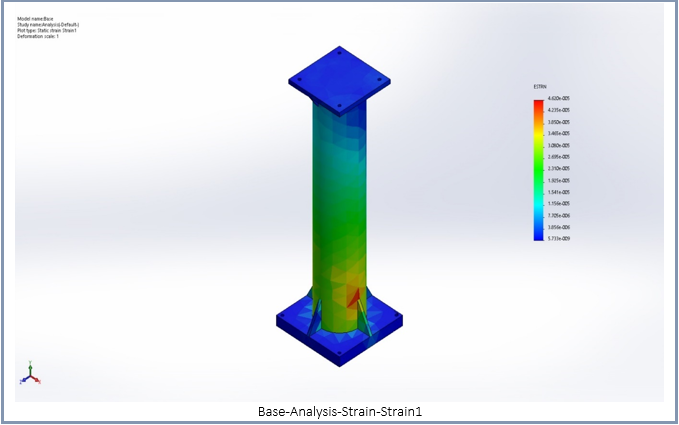
\includegraphics[scale=0.45]{zstrain}
	\caption{Solidworks representation for the base strain.} 
\end{figure}
\begin{center}
	The maximum strain is 7.56 and the minimum strain is 6.58.
\end{center}
\begin{figure}[H]
	\centering
	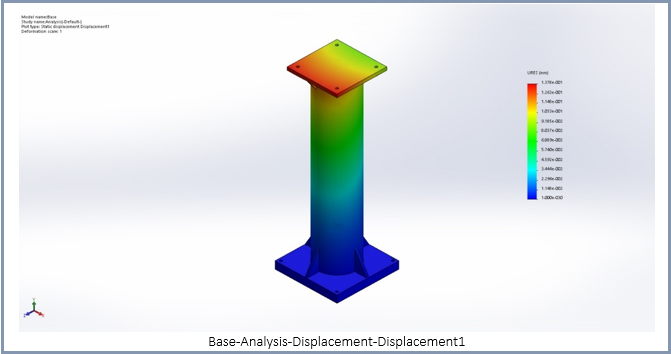
\includegraphics[scale=0.45]{zDisplacement}
	\caption{Solidworks representation for displacement at maximum loading.} 
\end{figure}
\begin{center}
	 Displacement of the base due to this forces is 2.7mm at maximum.
\end{center}


\newpage
\section{2.4 CAD Analysis Approach}

In Simulation and Analysis, you can test your designed product in real environment.In simulation process the model can be tested against parameters like static and dynamic response, fluid dynamic, heat transfer. It also supports thermal, fatigue, structural and motion analysis. 
\newline In our project, SolidWorks is used to obtain a CAD model for KR6 r900 sixx and to perform a motion analysis study on the model. In addition to designing a base to fix the robot arm, perform a stress analysis and creating an animation video of the model’s motion.

\subsection{Complete CAD Model}

\subsubsection{Searching for a suitable model}
All CAD models for KR6 r900 sixx on KUKA website or GrabCAD were step imported parts which are treated as a one body where joints can’t rotate therefore, motion study can’t be performed because it was impossible to add motors at the robot joints. The solution for this issue was obtained by converting step parts into assembly, which is done through several steps:
\begin{itemize}
	\item Open the .stp file part in SOLIDWORKS.  Select the file type to be .stp
	\item Click the OPTIONS tab, select Import multiple bodies as parts and click OK.
	\item Then click Open.
\end{itemize}
SolidWorks will create an assembly and create an individual part file for each multibody (Part1,Part2,Part3 etc.)
\begin{figure}[H]
	\centering
	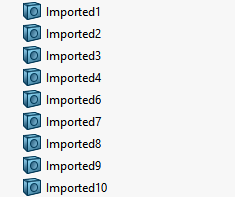
\includegraphics{Stepparts}
	\caption{Step parts}
\end{figure}

\begin{figure}[H]
	\centering
	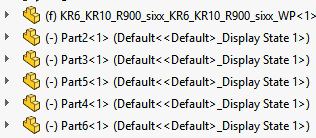
\includegraphics{assemblyparts}
	\caption{SolidWorks parts}
\end{figure}

\subsubsection{Modifications on CAD model}
\paragraph{Material and weights}
The robot material wasn’t specified and the model was a whole body, and the total mass for the robot was 33.74 Kg, which was not accurate, because the actual mass of the robot, according to the KR6 R900 sixx dimensions manual, must be approximately equal to 52Kg. This is achieved by making the model hollow, using the shell feature and adding to joins point masses similar to the real motors with mass approximate equal to motors masses. 

\begin{figure}[H]
	\centering
	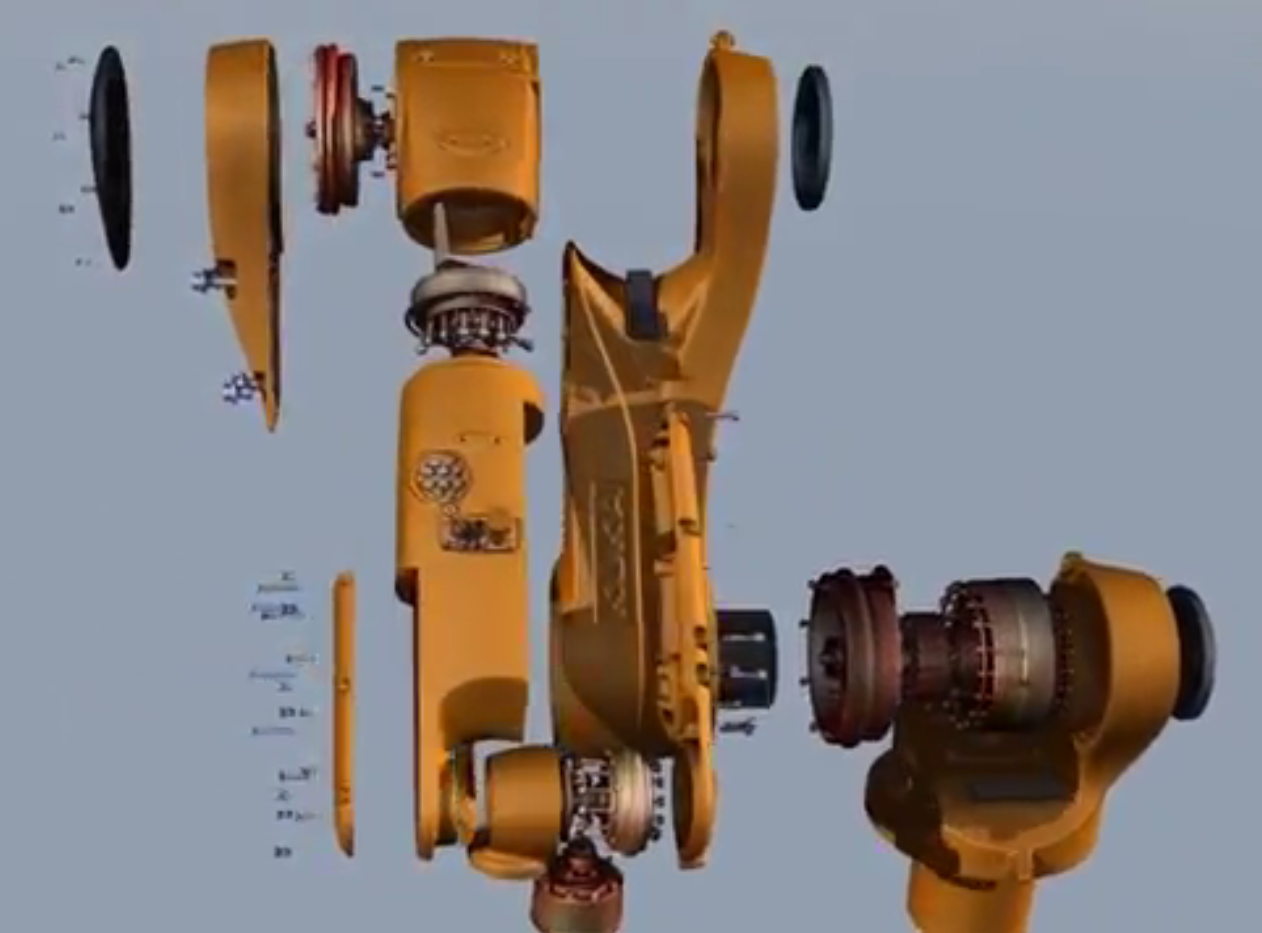
\includegraphics[scale=0.3]{KUKAmotor}
	\caption{KUKA motors}
\end{figure}

\begin{figure}[H]
		\centering
		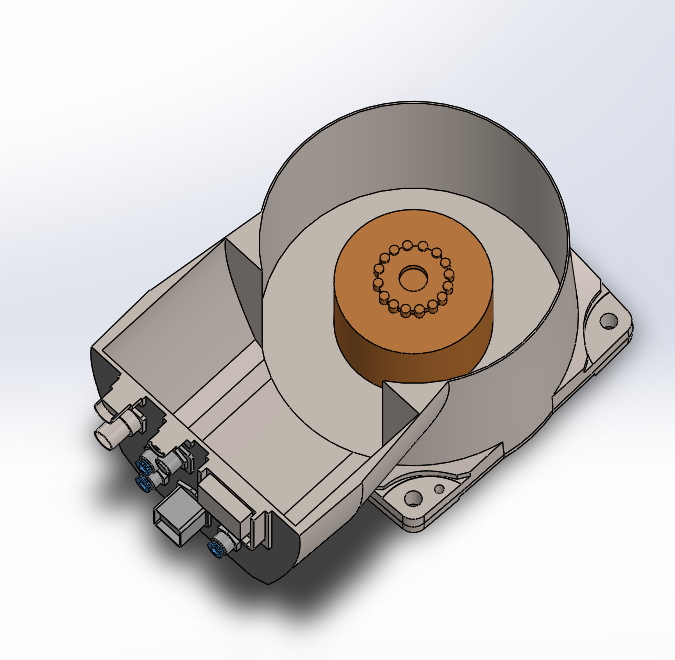
\includegraphics[width=0.6\linewidth]{Motor1}
		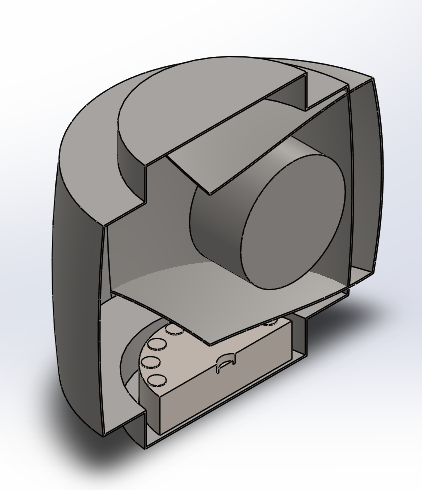
\includegraphics[width=0.4\linewidth]{Motor3}
	\caption{Motors model: Motors 1,2 and 3 model and Motors 4,5 and 6 model}
	\label{fig:fig}
\end{figure}

\begin{figure}[H]
		\centering
		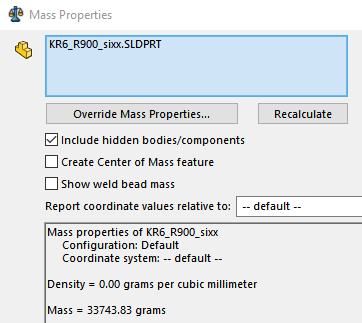
\includegraphics[width=0.6\linewidth]{Massbeforeadjust}
		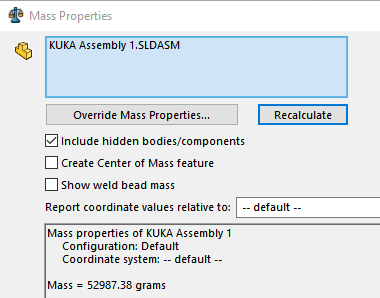
\includegraphics[width=0.45\linewidth]{Finalmass}
	\caption{The model mass: Old mass and final mass}
	\label{fig:fig22}
\end{figure}

\paragraph{Spindle}
In order to have a complete model for our graduation project, a router spindle and its holder were sketched to complete the existing KUKA model.

\begin{figure}[H]
	\centering
	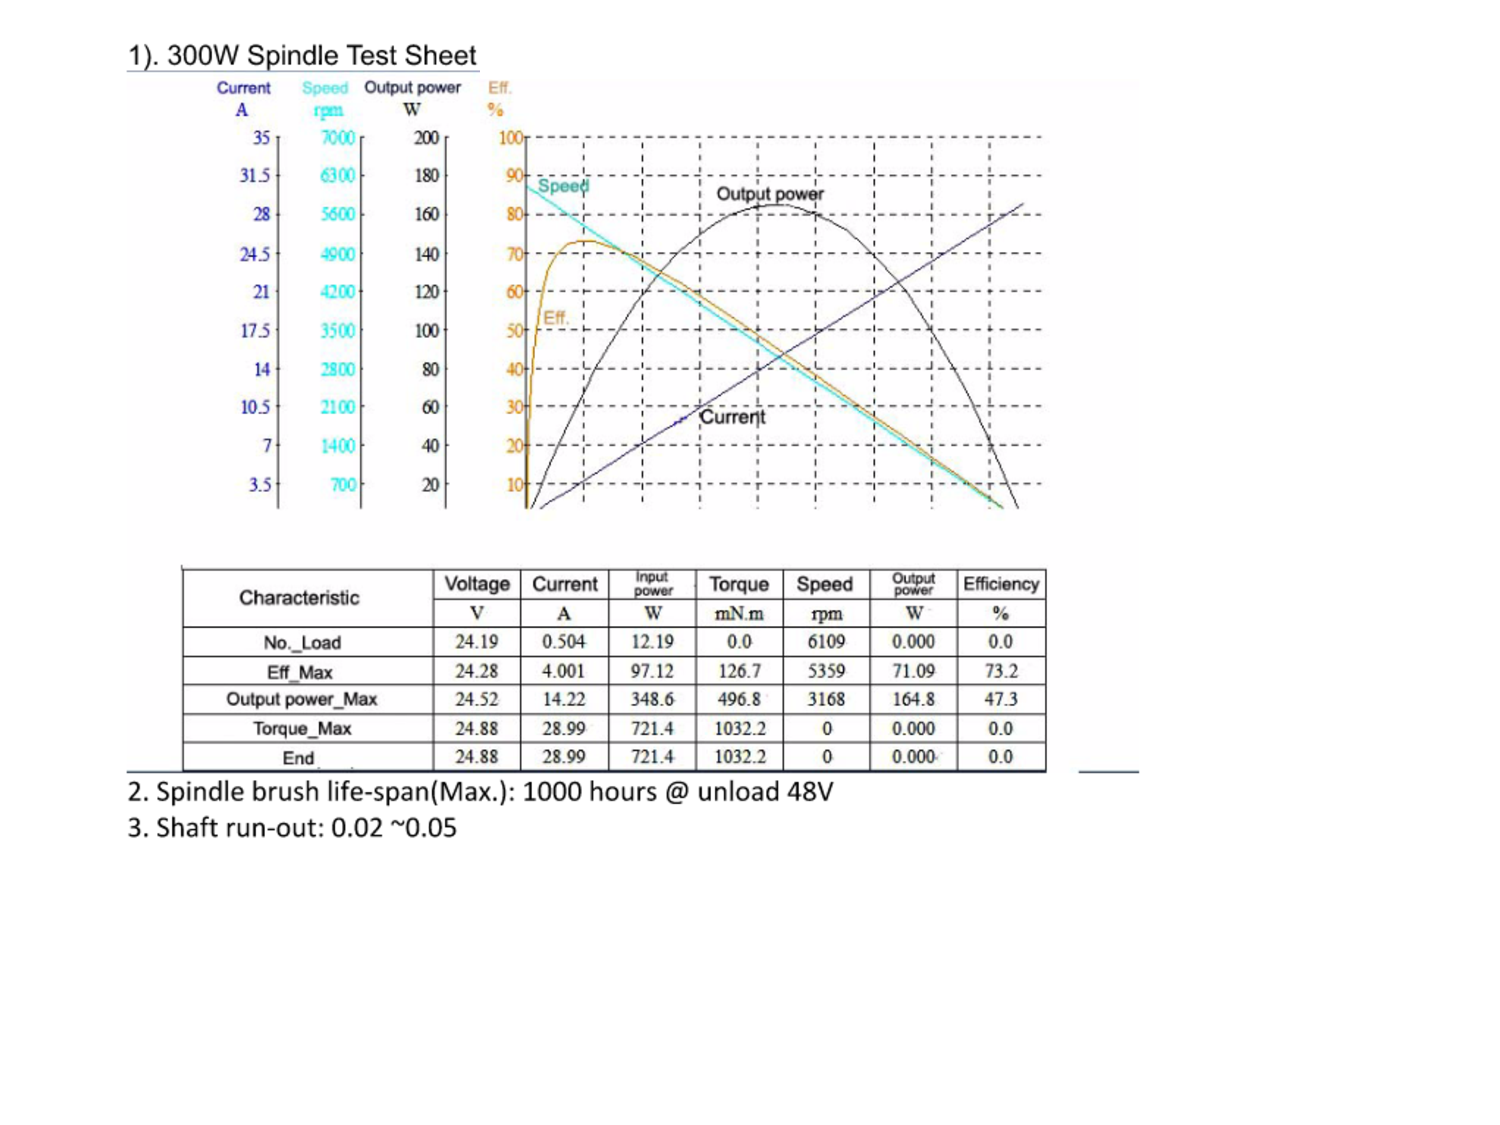
\includegraphics[scale=0.2]{spindle}
	\caption{Spindle model}
\end{figure}

\begin{figure}[H]
	\centering
	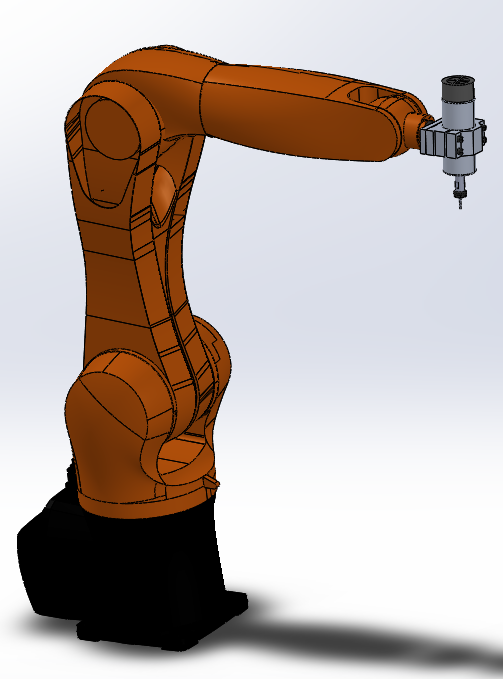
\includegraphics[scale=0.45]{FinalCADmodel}
	\caption{Final CAD model}
\end{figure}

\subsection{Motion studies}
Motion studies are graphical simulations of motion for assembly models. They simulate and animate the prescribed motion for a model. SolidWorks offer three different types of motion study, Animation, Basic Motion and Motion Analysis. They also offer mate controller that show, save the positions of assembly components at various mate values and degrees of freedom and create simple animations between those positions.
\smallskip
\newline Animation can be used to animate the motion of assembly. If you simply wish to create some nice visuals for presentation or marketing without consideration of mass and gravity effects, then animation is for you. 
\newline Basic Motion is an extra layer of complexity that takes into consideration the effects of mass, motors, springs, contact, and gravity on assemblies. 
\smallskip
\newline Motion Analysis is the top tier of motion study provides accurately simulation and analyze the motion of an assembly while incorporating the effects of Motion Study elements (including forces, springs, dampers, and friction). Motion Analysis can also be used to plot simulation results for further analysis.
\smallskip
\newline Therefore, Motion Analysis is used to simulate the model, generating results and plots of the simulation and Animation is used to make a video for motion.

\bigskip
\subsubsection{Animation study} 
Animation study is done to make an animation video of the moving parts with the use of limit mates. Limit angle mate is an advanced mate type that is performed by selecting two planes which rotate with respect to each other giving the desired range to mate and input a maximum and minimum value for the angle to specify the desired range of motion. Another advantage of limit angle is that it prevent collision between the moving parts.

\begin{figure}[H]
	\centering
	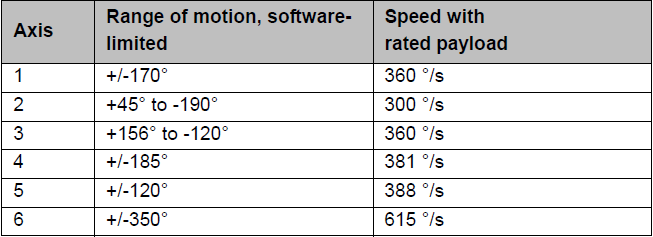
\includegraphics[scale=0.7]{Axesrangeofmotion}
	\caption{Axes range of motion}
\end{figure}

\bigskip
\subsubsection{Motion analysis}
On implementing motion analysis by adding a motor at the required location to start simulating the robot, a problem arose; the model exploded on running the simulation where some of the parts were separated from each other. This happened because of redundancy constrains. For Motion Analysis studies, having redundant mates is the equivalent of over-defining the model.  

\begin{figure}[H]
	\centering
	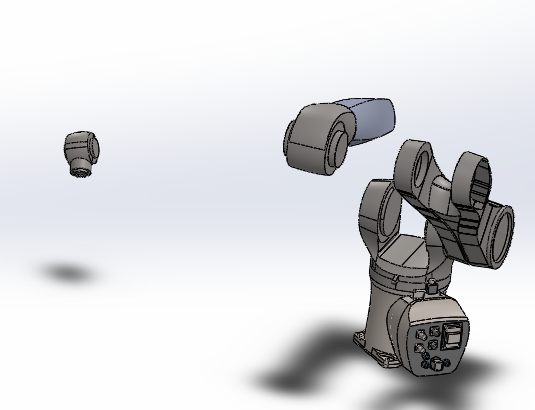
\includegraphics[scale=0.45]{Redundancyproblem}
	\caption{Redundancy constraint problem}
\end{figure}

This issue was solved by using mechanical mates of hinge type instead of standard mates. Hinge mate limits the movement between two components to one rotational degree of freedom. It has the same effect as adding a concentric mate plus a coincident mate and also limit the angular movement between the two components by adding limit angles. Reducing the negative effect of redundant mates on analysis.

\begin{figure}[H]
	\centering
	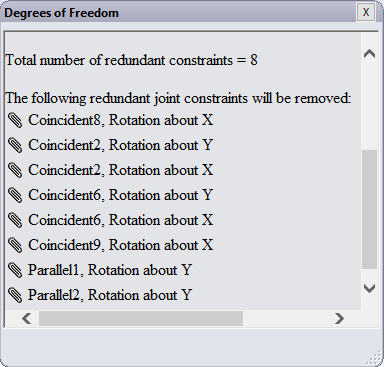
\includegraphics[scale=0.6]{redundancyconstrains}
	\caption{Presence of redundancy constrains}
\end{figure}

\begin{figure}[H]
	\centering
	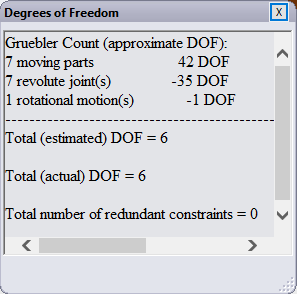
\includegraphics[scale=0.9]{zeroredandantcontraints}
	\caption{Zero redundant constraints}
\end{figure}
\smallskip
Now motors can be added to the model to perform any motion and results as motor torque, velocity, acceleration and force are generated.

\bigskip
\paragraph{Results of motion analysis study}] 
By assigning a motor to simulate the motion of axis and plotting the results to achieve this motion we found:
\begin{enumerate}
	\item Results of motor torque for axis 1 to move 100 degrees in 4 seconds:

	\begin{figure}[H]
		\centering
		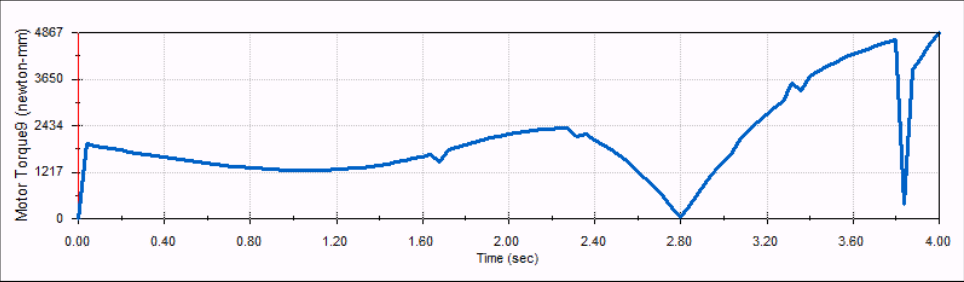
\includegraphics[scale=0.5]{Motor1torque}
		\caption{Motor 1 torque}
	\end{figure}
	
	\smallskip
Knowing that the actual motor torque for axis 1 is 4.5 N.m so the motion analysis result is approximate to actual torque. 
\newline Motor torque vary with time because of the motion of the links beyond the motor which has an effect on the torque by changing the loads carried by the motor.
\smallskip
	\item Motor 2 torque to move 60 degrees in 2 seconds:
	\begin{figure}[H]
		\centering
		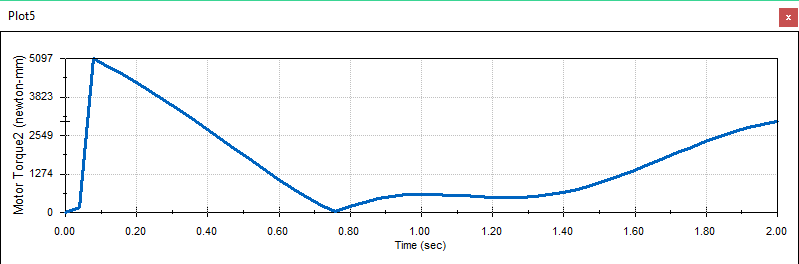
\includegraphics[scale=0.6]{Motor2torque}
		\caption{Motor 2 torque}
	\end{figure}
	
	Where the actual motor torque is 4 N.m

\smallskip
	\item Motor torque for axis 3 to move 75 degrees in 1.8 seconds:
	\begin{figure}[H]
		\centering
		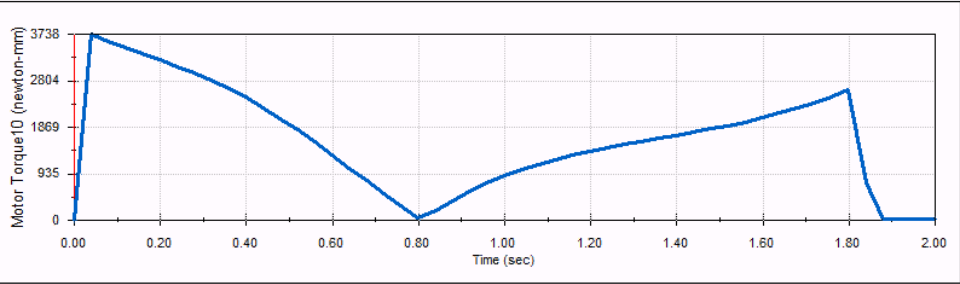
\includegraphics[scale=0.45]{Motor3torque}
		\caption{Motor 3 torque}
	\end{figure}
	
	Knowing that the actual motor torque for axis 3 is 3.5 N.m so the motion analysis result is approximate to actual torque.
\end{enumerate}

\bigskip
\paragraph{Trace path}
Motion analysis results and plots have a trace path option that can trace the path of a point in the assembly. The selected point is end mill vertex to create the curve feature that represent the motion of the links.  By assigning a data point motors to the joints whose data is imported from excel spreadsheet of file type .csv containing two columns, first represent time in seconds while other is degrees of rotation. The generated curve of adding this data to joints 1-5 is an arc shape.

\begin{figure}[H]
	\centering
	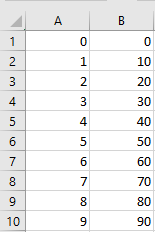
\includegraphics[scale=0.6]{datapoint}
	\caption{Used data point}
\end{figure}

\begin{figure}[H]
	\centering
	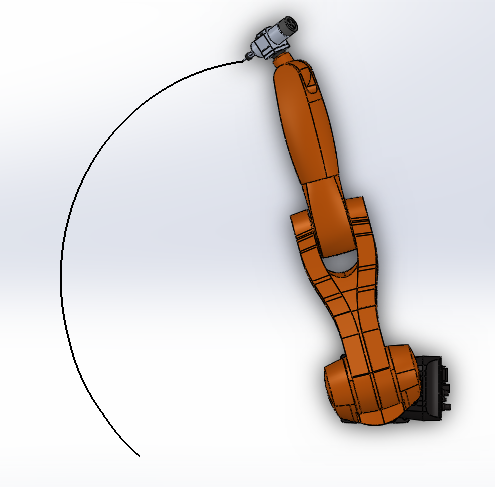
\includegraphics[scale=0.6]{Tracepathcurve}
	\caption{Created curve}
\end{figure}

%
%\end{chapter}
%    \end{document}
%==============================================================================

%Chapter 3: KUKA conditioning
%chapter 3 (already merged)
\chapter{KUKA conditioning} \label{ch:conditioning}
%HodaMahmoud
\documentclass{book}
\usepackage{graphicx}
\usepackage{float}

\begin{document}

	\begin{chapter}{KUKA conditioning} 
	\section{Robot Mastering}
	
	The Mastering operation calibrates the relationship between the position sensor, attached to each axis motor, and each axis angle defined for each robot. Mastering axes enables the definition of geometric parameters used to describe the analytic parameters of a robot’s geometric model. This helps in increasing the accuracy of the robot and correcting for discrepancies between design parameters and actual values.
	\newline
	Mastering the robot is performed by moving the each axis into a defined mechanical position, which is known as the “Mechanical zero position”. The zero position, which is defined by a reference notch, is an assignment to the axis drive angle. Whenever the robot moves from the mechanical zero position, its deflection represents the change in corresponding axis angle (0 increments for 0 degrees).
	\newline
	To locate the mechanical zero position of a robot axis precisely, the axes must be aligned to their pre–mastering position. The protective cap of the gauge cartridge is then removed and a dial gauge, or the supplied EMD, is fitted to it. 
	
		\begin{center}\textit{Note: The robot must be mastered in the same temperature conditions (either always cold or at operating temperature) to avoid inaccuracies.}
			

		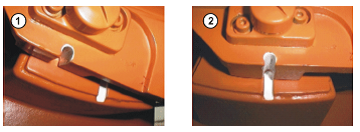
\includegraphics[scale=1.2]{mastering1}
		\caption{Moving an axis to pre-mastering position}
	\end{center}

	
	On passing over the reference notch, the gauge pin reaches its lowest point, the mechanical zero position is reached. The electronic measuring tool sends an electronic signal to the controller.
	
	Mastering can be performed through several methods; for older Robot versions it is performed using EMT, as for the KUKA AGILUS, mastering is done using one of these methods; EMD, dial gauge or MEMD. For our purpose, we used the MEMD supplied with the robot. The mastering positions are similar, but not identical, for all robots. Exact positions may vary between individual robots or single robot type. 
	
	
	\begin{center}
		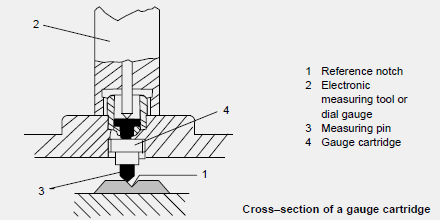
\includegraphics[scale=1]{mastering2}
		\caption{Moving an axis to pre-mastering position}
	\end{center}
	
		\subsection{Mastering using MEMD}
		Unlike Dial gauge mastering, which requires moving the robot manually to the mastering position, MEMD mastering offers automatic movement, done by the robot, to reach the mastering position. Mastering is performed first without a load then repeated using a load. The MEMD mastering tools are shown in the below picture.
		

		\begin{minipage}{0.8\textwidth}	
			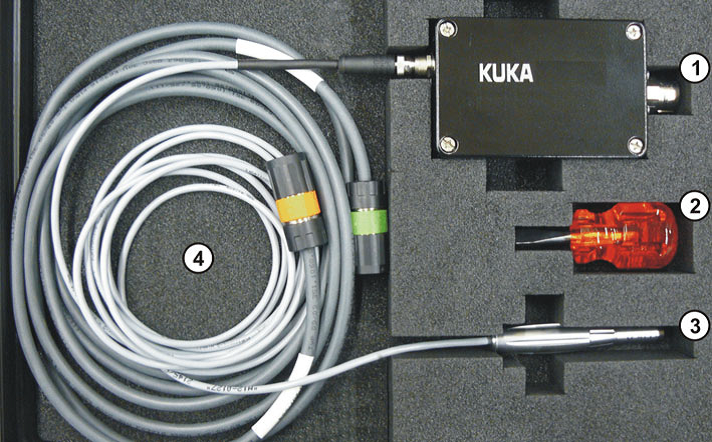
\includegraphics[scale=0.5]{mastering3}
			\begin{center}		
			\caption{MEMD kit}
			\end{center}
		\end{minipage} \hfill
		\begin{minipage}{0.5\textwidth}
			\begin{enumerate}
				\item MEMD box
				\item Screwdriver
				\item MEMD
				\item Cables
			\end{enumerate}
		\end{minipage}
		
		\bigskip
		\paragraph{Types of mastering}
		\begin{enumerate}
			\item First mastering (without a load).
			\item Tech offset (with a load and with saving the difference from first mastering being saved).
			\item Master load with offset is based on saving an offset value that can be used to calculate first mastering in case it was lost (used when required, carried out with a load for which an offset has already been taught. This type is used to check first mastering or to restore it in case it was lost).
		\end{enumerate}
		
		\paragraph{Precondition}
		\begin{itemize}
			\item There is no load on the robot; i.e. there is no tool, workpiece or supplementary load mounted.
			\item A1 to A5 are in the pre-mastering position.
			\item No program is selected.
			\item Operating mode T1
		\end{itemize}
		
		\paragraph{Procedure}
		\begin{enumerate}
			\item In the main menu, select Start-up > Master > EMD > With load correction > First mastering. A window opens. All axes to be mastered are displayed. The axis with the lowest number is highlighted.
			\item Remove the cover from connection X32.
			\item Connect the EtherCAT cable to X32 and to the MEMD box.
			\item Remove the protective cap of the gauge cartridge on the axis highlighted in the window.
			\item Screw the MEMD onto the gauge cartridge.
			\item Press Master.
			\item Press an enabling switch and the Start key.
			\item When the MEMD has passed through the reference notch, the mastering position is calculated. The robot stops automatically. The values are saved. The axis is no longer displayed in the window.
			\item Remove the MEMD from the gauge cartridge and replace the protective cap.
			\item Repeat steps 4 to 8 
		\end{enumerate}
	
		\paragraph{Mastering of A6}
		\begin{enumerate}
			\item Move A6 to the mastering position. A6 has very fine marks in the metal. Align these marks exactly with one another.
			\item In the main menu, select Start-up > Master > Reference.
			\item The option window Reference mastering is opened. A6 is displayed and is selected.
			\item Press Master. A6 is mastered and removed from the option window.
			\item Close the window.
			\item Disconnect the EtherCAT cable from X32 and the MEMD box.
		\end{enumerate}
		
		\fbox{\begin{minipage}{32em}
				For more information about the remaining mastering types (teach offset and mastering load with offset) and other mastering methods (using dial gauge and EMD), please refer to section “5.9 Mastering” in the provided manual “07-KSS\_82\_Software programming\_en”.
			\end{minipage}
		}
	\newpage		
	\section{Robot Calibration}
	Robot calibration is defined as identifying certain parameters in the robot’s kinematic structure, as an example; identifying relative position of robot links. Robot calibration can be performed through various methods, two of which are using a predefined and built-in calibration programs, or external methods (hardware and/or software) as RoboDK or advintec TCP. Calibration process differs in complexity from one method to another. 

	Calibration can be divided into three levels, depending on the type of modeled errors. The first of which models the differences between the actual and reported joint displacement values. This is also known as mastering. The second level, kinematic calibration, is related to the geometry of the robot and performing full geometric calibration, including angle offsets and joint lengths. The third level, non-kinematic calibration, models errors such as stiffness and friction.

	Calibration offers higher positioning accuracy for offline programmed robots. Accuracy means that the real position of the robot end effector corresponds better to the actual position calculated from the robot’s mathematical model. In the case of offline programming, pose accuracy is considered an important performance criteria.
		
	The calibration method used in out project is the first; using a predefined and built-in calibration program, which can be performed through different procedures in the KUKA platform, varying for tool and base calibration. For base calibration, these procedures are 3-point method, indirect method and Numeric input, and for tool calibration the procedures are XYZ 4-point method and XYZ reference method, both for TCP, ABC 2-point method and Numeric input. For the purpose of our project, the applied calibration procedures for both tool and base calibration were XYZ 4-point method and 3-point method respectively.
		
		\subsection{Tool calibration using XYZ 4-point procedure}
	
		
	

	%	\begin{minipage}{0.5\textwidth}
			The TCP of the tool to be calibrated is moved to a reference point from four different directions. The reference point can be freely selected. The robot controller calculates the TCP from the different flange positions. These four directions must be sufficiently different from one another (similar to the positions shown in the provided pictures).


\newline	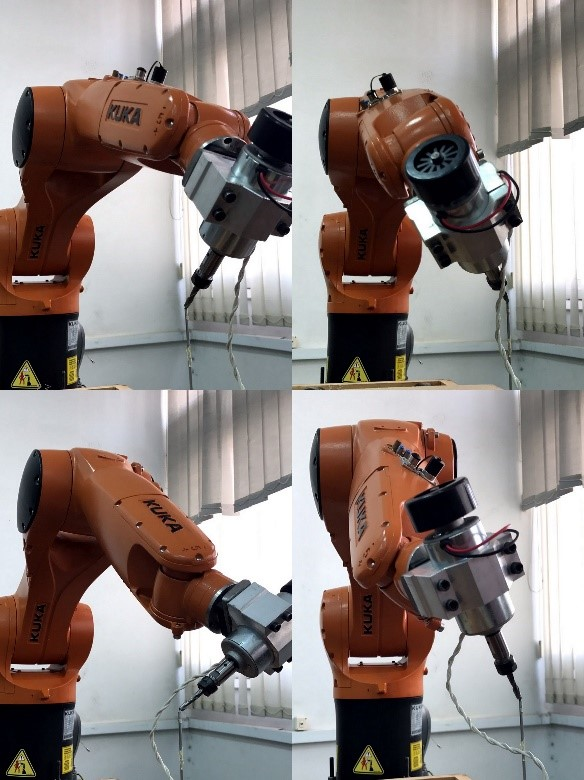
\includegraphics[scale=1]{calibration1}

		
		\paragraph{Precondition}
		\begin{itemize}
			\item A previously calibrated tool is mounted on the mounting flange.
			\item Operating mode T1
		
		\end{itemize}
		
		Preparation
		
		Calculate the TCP data of the calibrated tool:
		\begin{enumerate}
			\item In the main menu, select Start-up > Calibrate > Tool > XYZ Reference.
			\item Enter the number of the calibrated tool.
			\item The tool data are displayed. Note the X, Y and Z values.
			\item Close the window.
		\end{enumerate}
		
		Procedure
		\begin{enumerate}
			\item In the main menu, select Start-up > Calibrate > Tool > XYZ Reference.
			\item Assign a number and a name for the new tool. Confirm with Next.
			\item Enter the TCP data of the calibrated tool. Confirm with Next.
			\item Move the TCP to a reference point. Press Calibrate. Answer the request for confirmation with Yes. 
			\item Move the tool away and remove it. Mount the new tool.
			\item Move the TCP of the new tool to the reference point. Press Calibrate. Answer the request for confirmation with Yes.
			\item Enter the payload data. (This step can be skipped if the payload data are entered separately instead.)
				(>>> 5.12.3 "Entering payload data" Page 138)
			\item Confirm with Next.
			\item If required, coordinates and orientation of the calibrated points can be displayed in increments and degrees (relative to the FLANGE coordinate system).
			\item For this, press Meas. points. Then return to the previous view by pressing Back.
			\item Either: press Save and then close the window via the Close icon.
			Or: press ABC 2-point or ABC World. The previous data are automatically saved and a window is opened in which the orientation of the TOOL coordinate system can be defined.
		\end{enumerate}
		
		\subsection{Base calibration using 3-point method}
		
		During base calibration, the user assigns a Cartesian coordinate system (BASE coordinate system) to a work surface or the workpiece. The BASE coordinate system has its origin at a user-defined point. In 3-point calibration, the robot moves to the origin and 2 further points of the new base. These 3 points define the new base.
		
		Advantages of base calibration
		\begin{enumerate}
			\item The TCP can be jogged along the edges of the work surface or workpiece.
			\item Points can be taught relative to the base. If it is necessary to offset the base, e.g. because the work surface has been offset, the points move with it and do not need to be retaught.
		\end{enumerate}
		
		Precondition
		\begin{itemize}
			\item A previously calibrated tool is mounted on the mounting flange.
			\item Operating mode T1
		\end{itemize}
		
		Procedure
		\begin{enumerate}
			\item In the main menu, select Start-up > Calibrate > Base > ABC 3-point.
			\item Assign a number and a name for the base. Confirm with Next.
			\item Enter the number of the mounted tool. Confirm with Next.
			\item Move the TCP to the origin of the new base. Press Calibrate. Answer the request for confirmation with Yes.
			\item Move the TCP to a point on the positive X-axis of the new base. Press Calibrate. Answer the request for confirmation with Yes.
			\item Move the TCP to a point in the XY plane with a positive Y value. Press Calibrate. Answer the request for confirmation with Yes.
			\item If required, coordinates and orientation of the calibrated points can be displayed in increments and degrees (relative to the FLANGE coordinate system). For this, press Meas. points. Then return to the previous view by pressing Back.
			\item Press Save.
		\end{enumerate}
		
			\fbox{\begin{minipage}{32em}
				For more information about tool and base calibration, please refer to section “5.11 Calibration” in the provided manual “07-KSS\_82\_Software programming\_en”.
		 	\end{minipage}
		}
		\newpage
		\section{WorkVisual and LAN connection}
		The WorkVisual software package is the engineering environment for KR C4 controlled robotic cells. It offers the following functionalities:
		\begin{itemize}
			\item Configuring and connecting field buses
			\item Programming robots offline
			\item Configuring machine data
			\item Configuring machine data
			\item Editing the safety configuration
			\item Transferring projects to the robot controller
			\item Loading projects from the robot controller
			\item Comparing a project with another project and accepting differences where necessary
			\item Managing long texts
			\item Managing option packages
			\item Diagnostic functionality
			\item Online display of system information about the robot controller
			\item Configuring traces, starting recordings, evaluating traces (with the oscilloscope)
		\end{itemize}
		
			\paragraph{Hardware requirements:}
			Minimum requirements 
				\begin{itemize}
					\item PC with Pentium IV processor, min. 1500 MHz
					\item 512 MB RAM
					\item DirectX8-compatible graphics card with a resolution of 1024x768 pixels
				\end{itemize}
			Recommended specifications
				\begin{itemize}
					\item PC with Pentium IV processor and 2500 MHz
					\item 1 GB RAM
					\item DirectX8-compatible graphics card with a resolution of 1280x1024 pixels
				\end{itemize}
			\paragraph{Software requirements:}
				\begin{itemize}
					\item Windows 7 (Both the 32-bit version and the 64-bit version can be used).
					\item Or: Windows XP (32-bit version, with at least Service Pack 3, the 64-bit version cannot be used).
				\end{itemize}
			If the following software are not already installed on the PC, the installation wizard automatically starts their installation before preceding with the WorkVisual installation.
				\begin{itemize}
					\item .NET Framework 2.0, 3.0 and 3.5
					\item SQL Server Compact 3.5
					\item Visual C++ Runtime Libraries
					\item WinPcap
				\end{itemize}
			\subsection{WorkVisual Installation}
				\begin{enumerate}
					\item Start the program setup.exe.
					\item If the following components are not yet installed on the PC, an installation wizard opens:
						\begin{itemize}
							\item NET Framework 2.0, 3.0 and 3.5
							Follow the instructions in the installation wizard. .NET Framework is installed.
						\end{itemize}
					
					\item If the following component is not yet installed on the PC, an installation wizard opens:
						\begin{itemize}
						\item SQL Server Compact 3.5
						Follow the instructions in the installation wizard. SQL Server Compact 3.5 is installed.
						\end{itemize}
					
					\item If the following components are not yet installed on the PC, an installation wizard opens:
						\begin{itemize}
							\item Visual C++ Runtime Libraries
							\item WinPcap
							Follow the instructions in the installation wizard. Visual C++ Runtime Libraries	and/or WinPcap is installed.
						\end{itemize}
					\item The WorkVisual […] Setup window opens. Click on Next.
					\item Accept the license agreement and click on Next.
					\item Click on the desired installation type.
					\item Click on Install. WorkVisual is installed.	
					\item Once installation is completed, click on Finish to close the installation wizard.
				\end{enumerate}
					\fbox{\begin{minipage}{32em}
						For more information about installation, uninstallation and GUI of the WorkVisual software, please refer to Manual “KST\_WorkVisual\_en”.
					\end{minipage}
				}
			\subsection{LAN connection}
			In order to start file sharing process and to be able to use all functions of WorkVisual, a PC-Controller connection must be established. There are several ways to connect the KRC4 and KUKA-PC, one of which is setting up a local network for the connection of between several devices. This can be done by either setting static IPs for the connected devices and connecting them physically using a specified Ethernet cable, or by using a network router and assign dynamic IPs starting from a specified value, with specified number of connected devices. 
			\newline	
			\paragraph{To obtain and/or change IP values for the PC}
			\begin{enumerate}
				\item Open "Network and sharing center" 
				\item Choose "Change adapter settings"
				\item Right click "Ethernet connections"
				\item  Choose "Internet protocol version 4 (TCP/IPv4)"
				\item  Choose "Properties"
				\item Next you either set static IPs or choose dynamic IPs to be set, in our case by the router.
			\end{enumerate}
			
			\fbox{\begin{minipage}{32em}
					The following address ranges are used by default by the
					robot controller for internal purposes. IP addresses from
					this range must not therefore be assigned by the user.
					\begin{itemize}
						\item 192.168.0.0 … 192.168.0.255
						\item 172.16.0.0 … 172.16.255.255
						\item 172.17.0.0 … 172.17.255.255
					\end{itemize}
					
				\end{minipage}
			}
			
			\paragraph{LAN Configuration steps}
			\begin{enumerate}
				\item Connect the PC and the KRC4 to the router using regular Ethernet cables.
				\item Access the router configuration page using the given data on the back of the router. (the router used in our case is TP-LINK, with username and password both being admin)
				\item In the Interface setup change the LAN settings to your preferred values
				\item It is preferred to set the starting IP address similar to that of the KRC4 (172.31.147) to avoid conflicts. Network gateway value is (172.31.1.1) and subnet mask (255.255.0.0), all other settings shall remain unchanged.
				
				\begin{center}
					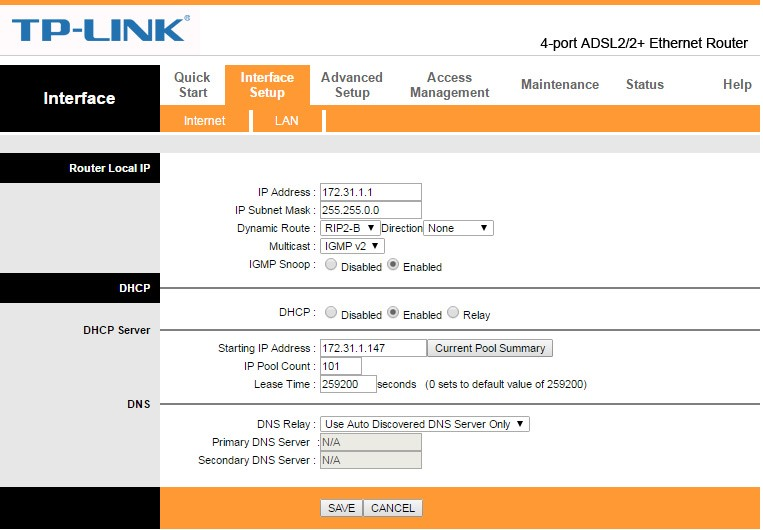
\includegraphics[scale=0.37]{network1}
				\end{center}
				
		
				
				\item After changing these values, the IP address used to access the router settings will change from (192.168.1.1) to the set gateway value (172.31.1.1) but with the same user name and password.
				
				fig6
				
				\begin{center}
				\includegraphics[scale=0.37]{network2}
				\end{center}
				
				\item The connection is now established and can be verified by checking the router LEDs
			\end{enumerate}
		
	\newpage
	\section{Installation of KUKA.Sim Pro}
	KUKA.Sim Pro is used for the complete offline programming of KUKA robots. This product allows the analysis of cycle times and the generation of robot programs. It also enables a real-time connection to the virtual KUKA robot controller (KUKA.OfficeLite). KUKA.Sim Pro is additionally used for building parametric components and defining kinematic systems, which can also be used in KUKA.Sim Layout and KUKA.Sim Tech. KUKA.OfficeLite is included in the KUKA.Sim Pro package. CAD importers are available as an option. This requires a purchasable license for each import interface. 
	


	\begin{center}
	\includegraphics[scale=0.25]{simpro1}
	\end{center}
	 
	 \paragraph{Requirements}
	 	\begin{itemize}
	 	\item The minimum requirements for the computer are a 2 GHz CPU and 2 GB RAM, and an OpenGL-capable graphics card with at least 512 MB RAM and a resolution of 1024 x 768 pixels or a similarly specified notebook.
	 	\item Supported operating systems are WIN XP - 32-bit or WIN 7 - 32/64-bit.
	 \end{itemize}
 
 	\subsection{Installation}
 		\begin{enumerate}
 			\item Start the setup file “.exe”
 			\item Read the agreement and activate the check box “I accept ...”
 			\item Select “Install” to start installation.
 			\item Select “Install” to complete installation
 		\end{enumerate}
 	
 	\paragraph{Installing the component library }
 	After installation of the KUKA.Sim software product, the component library is installed with the following program: SetupKUKASimLibrary\_2.2.0\_Buildx.exe The procedure is very similar to the installation of the software products. Simply follow the instructions given.
 	The KUKA.Sim component library contains over 1,000 typical layout components (robots, grippers, fences, etc.), various demo layouts and tutorials for KUKA.Sim. Although the KUKA.Sim products still work without the component library installed, it is strongly recommended that the component library is installed in order to be able to create layouts quickly and easily.
 	
 	\subsection{License types}
 	There are different types of licensing for the KUKA software. License types are determined and verified in accordance with the purchase made from KUKA Roboter GmbH. 
 	The software licensing concerning the KUKA arm at Zagazig university is an educational bundle license. The serial number for the license is found in the booklet of the KUKA.Sim Pro CD. Information about different licensing bundles are obtained by contacting KUKA Roboter GmbH by email
 	\textbf {simulation@kuka-roboter.de.}
 	Further details about the steps of obtaining the serial key, for different commercial bundles,  are found on page 13 of (KUKA.Sim 2.2- Installation-en) manual.
 	The serial number associated with this purchase is: \textbf {K5P22-N174H-AW7KY-9}
 	
 		\subsubsection{Stand-alone License}
 		The license is on the PC on which KUKA.Sim is used. The license key is then valid for this PC only. It can also be transferred to a different PC, but cannot be used on a two different PCs at the same time, or when either of the two PCs is off.
 		
 		\subsubsection{Network License}
 		Network licenses provide a flexible way of using KUKA.Sim on more than one PC. When a license is requested by a PC, this license is then allocated to this PC. When KUKA.Sim is closed, the license becomes available again and can be accessed by other PCs. 
 		A license server is required to manage the network licenses. When KUKA.Sim Pro is started, the computer’s identity (IP address, please refer to \textbf {LAN connection} in manual Section “WorkVisual \& LAN connection”) is required occasionally, however, KUKA.Sim Pro needs to check with the local license server to make sure that KUKA.Sim Pro and server are on the same PC, which is required in the network license configuration.
 	
 				\paragraph{Requesting a license file manually}
 					\begin{enumerate}
 						\item Start the installation of KUKA.Sim Pro 
 						\item Enter the license key
 						\item Select “Activate manually” and save the request file
 						\item Go to the Visual components customer portal and use the given email and password, mentioned in the previous section, to login.
 						\item On the website, choose Manual Licensing, upload the request file and confirm.
 						
 						\begin{center}
						\includegraphics[scale=0.35]{simpro2}
 						\end{center}
 					
 					
 						
 						\item The license should be activated.
 						\item Download the license (.dat) file and click Finish. Please complete the installation steps of the license server before proceeding with the next steps.
 						\item The license (.dat) file should be loaded into the license server, not the KUKA.Sim Pro interface, in order to complete the activation process. 
 						
						\includegraphics[scale=0.37]{simpro3}
						 						
 						\item After this process is completed, the network server interface should appear as follows
 					\end{enumerate}
 				
 				\paragraph{Installing the license server}
 				\paragraph{Requirements}
 				“Microsoft Management Console” (MMC) must be installed on the license server. The software can be downloaded from the Microsoft website. In addition, “.NET framework 3.5” or higher should be installed. 
 				
 				\paragraph{Installation}
 					\begin{enumerate}
 						\item The license server is started via “Start > Programs > Visual Components > Visual Components License Server > Visual Components License Server Manager”.
 						\item Choose “Server settings” from the left panel, make sure that the license server is started, if not, click Start to activate it. The port number value is 5093.
 						\item On the left-hand side, select “Product keys” in order to enter the license key.
 							\begin{itemize}
 								\item The right-hand side changes and “Enter product key...” is offered. Click on this.
 								\item A window is opened in the center, in which the license key can be entered.
 								\item If manual licensing is being performed using a license file, this license file must be loaded with “Load license file...”.
 							\end{itemize}
 						\item Enter the license key and confirm with OK.
 					\end{enumerate}
 				
 				For network licensing, an account linked with the purchase is created on the Visual Components website (http://www.visualcomponents.com/). In the specified customer portal (https://portal.visualcomponents.net/website/Login.aspx), sign in with the email hodaeltahawy@gmail.com and password quails@123 . In the “My Products keys” tab, you will find the product key for KUKA.Sim Pro on the KUKA-PC device, at the Mechatronics lab. The license is already activated and will only require renewal after a period of 400 days starting 3-12-2016, which is on 7-1-2018. 
	 
	 \newpage
	 \section{End-effectors installation}
	 	\subsection{Pneumatic gripper}
	 	The KUKA AGILUS offers numerous options for different end-effectors installations. One of the most common end effectors is a gripper, whether it be vacuum, pneumatic, hydraulic or servo-electric grippers. We are concerned with pneumatic grippers, which operate using air pressure. When air pressure is applied on the pistons, the gripper closes. When the pressure is released the gripper opens. The only way to manage the force in the gripper is to manage the air pressure in the air intake (or valve). The gripper used in our study is the SOMMER automatic GP 404 NC-C We also had the opportunity to work with one of KUKA Roboter’s Application software; Gripper\&SpotTech. These are ready-made software packages created for different industrial applications. Optional features can be installed on the controller easily and quickly and can also be tailored to the specific production environment. 
	 	
	 	These software include, and not limited to, KUKA.ArcTech, which enables implementation and programming of applications for arc welding and plasma cutting, KUKA.ConveyorTech, which automatically adapts the actions of the robot to the motion of an assembly line or conveyor belt and KUKA.CNC, which links the CNC and robot directly to each other. As a result, they can be operated like a conventional CNC controller.
	 	
	 	Pneumatic grippers can be used in many applications, some of which include assembly purposes, Labs automation, and on mobile robots.
	 	
	 	This software package offers numerous advantages, including:
	 		\begin{itemize}
	 			\item 16 freely configurable grippers
	 			\item 16 freely configurable grippers
	 			\item Gripper conditions statically and dynamically monitored
	 			\item Unlimited user-defined gripper icons
	 			\item Unlimited user-defined gripper icons
	 			\item Graphical user interface with indicator lamps, a status display and online adaptation
	 			\item Adaptation via WorkVisual 4.0 and on the smartPAD for production-relevant elements
	 		\end{itemize}
 		\newpage	
 		\subsubsection{Gripper connection}
 		The gripper is connected to the air supply through the Air 1 port located on link 3 (The port is shown in the following picture). This port is connected internally to Air 1 port on the back of the robot arm, which in turn is connected with the air compressor.
 		\newline
 			\begin{minipage}{0.5\textwidth}	
 			\includegraphics[scale=0.05]{gripper1}
 		\end{minipage} \hfill
 		\begin{minipage}{0.6\textwidth}
 			\includegraphics[scale=0.6]{gripper2}
 		\end{minipage}
 		

 		\bigskip
 		In order for these ports to be operative, the connection between the ports and the controller must be activated, this is performed using mapping. Mapping can be simply described as the process of creating a link or a connection between ports on the robot arm and inner components in the controller in order to use them in control purposes, in our case operating the gripper. Mapping is performed through WorkVisual through the steps mentioned below.
 			\begin{enumerate}
 				\item get current project from robot using workvisual
 				\item save it as different file name
 				\item activate project in work visual (by double clicking on Controller<kss version>)
 				\item open I/O mapping
 				\item leave left pane on KRC (those are I/Os that robot programs can access), and click on inputs
 				\item move right pane to Fieldbus (those are physical I/O), then highlight EM8905 module (this is I/O card inside agilus arm)
 				\item map inputs of EM8905 to robot inputs of your choice
 				\item repeat steps 5.6.7 for outputs
 				\item on the robot login as Expert or higher (Expert will work in this case since we did not modify safety configuration)
 				\item deploy modified project to robot and activate it (on robot).
 				You should have something like on image below. 
 			\end{enumerate}
 		\begin{center}
 			\includegraphics[scale=0.5]{gripper3}...
 		\end{center}
 	Six valves are mapped to ports:
 	\newline
 		\begin{minipage}{0.5\textwidth}
 			\begin{enumerate}
 				\item 1A
 				\item 2A
 				\item 3A
 				\item 1B
 				\item 2B
 				\item 3B
 				\item R (relief/exhaust) 
 			\end{enumerate}	
 	\end{minipage} \hfill
 	\begin{minipage}{0.5\textwidth}
 			\includegraphics[scale=0.4]{gripper4}
 	\end{minipage}
 
 	\newpage
	\textbf{Configuring predefined grippers}

	\bigskip

	\begin{minipage}{0.5\textwidth}
	Gripper settings can be changed using smart pad. In the main menu, select Configure > I/O > Gripper. A window opens (shown in figure), inside it you’ll find a list of the predefined grippers, select the desired gripper number with Next or Previous. 
	\newline
	You can change number of grippers )1), Name of gripper (2), Type of gripper (3), designation of gripper type (4), Assignment of the output numbers (5), Assignment of the input numbers (6) and Switching states (7). 
	\newline
	The third cell, designated for the type of gripper is explained in the following section, Predefined gripper types.
	\end{minipage} \hfill
	\begin{minipage}{0.6\textwidth}
		\includegraphics[scale=0.4]{gripper5}
	\end{minipage}
 		
 	\paragraph{Predefined gripper types}
 	There are five predefined gripper types in Gripper\&SpotTech. If these types are not sufficient, additional gripper functions can be programmed.
 		\begin{itemize}
 			\item Type 1: Single-element gripper, static, open/closed
 			\item Type 2: With mid-position valve
 			\item Type 3: Vacuum gripper with 2 valves
 			\item Type 4: Vacuum gripper with 3 valves
 			\item Type 5: Single-element gripper with pulse valves, open/close
 		\end{itemize}
 			\fbox{\begin{minipage}{32em}
 				More information about the specifications of each type and user specified grippers can be found in manual “KST\_GripperSpotTech\_32\_en”.
 			\end{minipage}
 		}
 		\newcommand{}[a
 		\paragraph{Gripper operation}
 		Manual gripper control can be performed using technology keys on smart pad. The settings for the technology keys are already set for this gripper and appear with the following icons on the smart pad screen, next to the assigned buttons. 
 		
 	\begin{center}
 		\includegraphics[scale=0.35]{gripper8} 
 	\end{center}
 \newline
 The gripper is opened or closed using these buttons, after pressing the enable buttons on the back of the smart pad. They can also controlled inside KRL programs in inline form through the following command
 \begin{center}
 	\includegraphics[scale=0.7]{gripper9}
 \end{center}
 
 	\paragraph{Where}
 	\begin{enumerate}
 		\item Choosing the desired gripper from a list of predefined grippers in settings
 		\item Set the state of the gripper, whether to open or close
 		\item CONT: Execution in the advance run
 		\item Box only available if CONT selected.
 			\begin{itemize}
 				\item START: The gripper action is executed at the start point of the motion.
 				\item END: The gripper action is executed at the end point of the motion.
 			\end{itemize}
 		\item Box only available if CONT selected.
 			Define a wait time (-200:200 ms), relative to the start or end point of the motion, for execution of the gripper action.
 		\item Box only available if [blank] selected.
 		Data set with gripper parameters
 	\end{enumerate}
 
 \subsection{Electric spindle}
 For the purpose of milling, a spindle was attached as an end effector to perform this process. The spindle used was a simple ON/OFF spindle, which required no control signals, so it merely needed to be attached to the end effector and to an external power supply. 
 
 \paragraph{Spindle attachment }
 For the spindle to be attached to the sixth axis of the robot, a metal linkage was designed and manufactured to fit both the spindle and the mounting surface on the sixth axis. The first picture shows the mounting surface of the sixth axis of the robot. The second shows the metal linkage after being installed to the mounting surface. The Third and fourth pictures shows the spindle’s metal holder. 
 
 \begin{center}
 	\includegraphics[scale=0.08]{spindle1}
 \end{center}

\paragraph{Spindle connection}
The power supply of the spindle is connected to port XPN1 on the fourth axis, whose output is internally linked to a similar port XPN1 on the back side of the robot. The port contains four openings or smaller ports; the positive wire is connected to the two right-hand side ports and the negative side to the left-hand side ports. The ports are shown in the picture below.

  \begin{center}
 	\includegraphics[scale=0.06]{spindle2}
 \end{center}

\paragraph{Spindle specifications }

The spindle used is an Air cooled spindle, with a 300W CNC Spindle Motor, supplied by a 220 voltage source, with adjustable speed through the attahced knob. The spindle must operate with full speed during the milling process. Further information about the spindle can be found in the resources in the references. 

\paragraph{End mill used for machining}

The end mill used is a double blade 6 mm Carbide blade. A 6 mm collet was used to attach the end mill to the spindle. A collet is a subtype of chuck that forms a collar around an object to be held and exerts a strong clamping force on the object when it is tightened, usually by means of a tapered outer collar. Both the end mill and the collet can be changed for different milling purposes, as an example, a smaller end mill can be used to obtain a higher level of fine details that larger end mills can’t offer, while larger end mills can be used to remove more material or perform faster in basic milling operations that does not require a high level of details. 

 
 
 
	\end{chapter}
\end{document}
%==============================================================================

%Chapter 4: Robot Programming
%chapter 4 (needs remerge)
\setchapterpreamble[o]{%
    \dictum[Joseph Addison, \textit{(English essayist, poet, and politician, 1672--1719), Spectator, No. 253}]{% source: http://todayinsci.com/A/Addison_Joseph/AddisonJoseph-Quotations.htm
        ``It is impossible for us, who live in the latter ages of the world, to make observations in criticism, morality, or in any art or science, which have not been touched upon by others. We have little else left us but to represent the common sense of mankind in more strong, more beautiful, or more uncommon lights.''}\vspace{0.1em}}
\chapter{Robot Programming} \label{ch:programming}
\documentclass[a4paper]{report}
\usepackage{graphicx}
\usepackage{ragged2e}
\usepackage{xcolor}
\usepackage[nottoc]{tocbibind}
\setcounter{secnumdepth}{3}
\setcounter{tocdepth}{3}
\usepackage{amssymb,amsmath,amsthm}
\pagestyle{empty}


\usepackage[style=authoryear,sorting=none]{biblatex}

\begin{document}
	
%	\begin{Robot Programming}
\tableofcontents
\newpage		
		
\section{Coordinate systems}
\subsection{Axis specific}

\subsection{Cartesian}
\subsubsection{Coordinate systems in conjunction with robots}
The following Cartesian coordinate systems are defined in the robot controller:
\begin{itemize}
	\item WORLD Coordinate System
	\newline
	Fixed, rectangular coordinate system whose origin is located at the base of the robot. It is the root coordinate system for the ROBROOT and BASE coordinate systems.
	By default, the WORLD coordinate system is located at the robot base.
	\item ROBROOT Coordinate System
	\newline
	Fixed, rectangular coordinate system whose origin is located at the base of the robot. It is the root coordinate system for the ROBROOT and BASE coordinate systems.
	By default, the WORLD coordinate system is located at the robot base.
	\item BASE Coordinate System
	Fixed, rectangular coordinate system whose origin is located at the base of the robot. It is the root coordinate system for the ROBROOT and BASE coordinate systems.
	By default, the WORLD coordinate system is located at the robot base.
	\item TOOL Coordinate System
	\newline
	a Cartesian coordinate system which is located at the tool center by default, the origin of the TOOL coordinate system is located at the flange center point. The TOOL coordinate system is offset to the tool center point by the user

\end{itemize}

\begin{figure}[h]
	\caption{KUKA robot coordinate systems}
	\centering
\includegraphics[scale=0.7]{kuka_coordinate_system.jpg}
\end{figure} 
\newpage
\section{KUKA Robot Language (KRL) Quick Guide}
KRC 4 controller uses KRL KUKA programming language.
\subsection{Variables and Declarations}
All system variables start with \textdollar sign, mind not starting any "user-defined" name with this sign to avoid syntax errors.
\vspace{0.5cm}
\subsubsection{Names in KRL}
\begin{itemize}
	\item Can have a maximum length of 24 characters
	\item Can consist of letters(A - Z), numbers(0 - 9) and the special characters '\textdollar'.
	\item Must not begin with a number.
	\item Must not be a keyword.
\end{itemize}
\subsubsection{Declaration and initialization of variables}
\begin{itemize}
	\item Variables (simple and complex) must be declared in the SRC file before the INI line and initialized after the INI line
	\item Variables can optionally also be declared and initialized in a local or global data list. 
	\item Every variable is linked to specific data type.
	\item The data type must be declared before use.
	\item The keyword for the declaration is DECL. It can be omitted in case of the four simple data type	
	\item In order to place syntax before the INI line, the DEF line must be activated:
	
	\centering	\textbf{  Open file \textgreater Edit \textgreater View \textgreater DEF line}
\end{itemize}

\fbox{\begin{minipage}{32em}
		
		DEF program name ( )
		\newline
		DECL data type user defined variable
		\newline;  declaration section of  variables
		\newline
		INI 
		\newline; Initialization section of user defined variables.
		\newline…
		\newline; Instruction Section
		\newline
		...
		\newline
		END
		
	\end{minipage}
	
}
\subsubsection{Simple Data types }
 
\begin{table}[h!]
	\centering
\begin{tabular}{| p{2cm} |p{3cm}|p{3cm}| p{2cm}| p{2cm}|}
	\hline
	\large Data Type & \large Integer & \large Real &\large Boolean &\large Character\\
	\hline
	\large Keyword & \large INT & \large REAL &\large BOOL &\large CHAR\\
	\hline
	\large Meaning & \large Floating point number & \large Logic state &\large Boolean &\large Character\\
	\hline
	\large Range & \large $-2^31 … 2^31-1$ & \large $±1.1E-38 … ±3.4E+38$ &\large TRUE, FALSE &\large ASCII character\\
	\hline
	\large Example & \large 2 & \large 4.23 &\large TRUE &\large C\\
	\hline

\end{tabular}
	\caption{is an example of KRL Data Types}
\label{table:1}
\end{table}
\newpage

\large {\textbf {Structure Types}}

\begin{itemize}

	\item AXIS: A1 to A6 are angle values (rotational axes) or translation values (translational axes)
		\vspace{.2cm}
		\newline
	\fbox{\begin{minipage}{32em}
			\centering
			{Axis: A1 .., A2 .., A3 .., A4, A5 .., A6 .. }
		\end{minipage}
	}
\vspace{.2cm}
	\item FRAME: X, Y, and Z are space coordinates, while A, B, and C are the orientation of the coordinate system.
		\vspace{.02cm}
	\newline

	\fbox{\begin{minipage}{32em}
			\centering
			{FRAME: X .., Y .., Z .., A .., B .., C .. }
		\end{minipage}
	}
\newline

\item POS and E6POS:  S (Status) and T (Turn) define axis positions unambiguously
\vspace{.2cm}
\newline
	\fbox{\begin{minipage}{32em}
		\centering
		{POS: X .., Y .., Z .., A .., B .., C .., S ..., T }
	\end{minipage}
	
}
\end{itemize}

\vspace{0.05cm}

	\section{Motion Programming}
\subsection{Motion Types}
The robot can move in various motion types. Paths are created according to the operation of each axis. Thus, the robot can be controlled to create either linear or circular path.
\subsubsection{Axis-specific motion}
	   The robot guides the TCP along the fastest path to the end point. The fastest path is generally not the shortest path and is thus not a straight line. The first motion in the program must be PTP as status and turns are only evaluated here.
	   The coordinates of the end point are absolute.
	   \paragraph{characteristics}
	   
	  
	   \begin{itemize}
	   	\item smooth motion
	   	\item Robot can move from start to end singularity free. As long as both the starting and ending points are in the working envelope, the robot will get to the end point without collision or sudden movement. 
	   	\item	Control is much simpler than continuous path control. 
	   \end{itemize}
   \begin{figure}[h]
   	\caption{PTP Motion}
   	\centering
   	\includegraphics[scale=0.9]{ptp.png}
   \end{figure} 
	   
 \subsubsection{CP motion}
 \paragraph{LIN Motion}
 Motion at a defined velocity and acceleration along a straight line.  This motion requires the programmer to “teach” one point.  The robot uses the point defined in the previous move as the start point and the point defined in the current command as the end point and interpolates a straight line in between the two points.
 
 \begin{figure}[h]
 	\caption{LIN Motion}
 	\centering
 	\includegraphics[scale=0.9]{LINmotion.png}
 \end{figure}
\paragraph{CIRC Motion}
Motion at a defined velocity and acceleration along a circular path or a portion of a circular path.  This motion requires the programmer to “teach” two points, the mid-point and the end point.  Using the start point of the robot (defined as the end point in the previous motion command) the robot interpolates a circular path through the mid-point and to the end point.
\begin{figure}[h]
	\centering
	\caption{CIRC Motion}
	\includegraphics[scale=0.9]{CIRCmotion.png}
\end{figure} 
\subsection{Approximate Positioning}
Approximate positioning of motion means that the next programmed point will not be exactly reached. This can help to shorten cycle times
 \begin{figure}[h]
	\caption{Speed Profile:
	\newline a) If all points approached exactly
	\newline b)In  case of approximate positioning of the points}
	\centering
	\includegraphics[scale=0.9]{approximateAdv.png}
\end{figure}
\begin{figure}[h]
	\caption{Approximate positioning of an auxiliary points}
	\centering
	\includegraphics[scale=0.9]{apppos.png}
\end{figure}
\subsubsection{PTP-PTP approximate positioning }
For the purposes of PTP approximate positioning,the controller calculates the distances the axes are to move in the approximate positioning range, and plans velocity profiles for each axis which ensure tangential transition from the individual instructions to the approximate positioning contour.
\vspace{0.3cm} 
\newline System Variable, \textdollar APO.CPTP enables the start of approximate positioning to be specified as a percentage of these maximum values.
The approximate positioning of a point is displayed in the PTP command by adding the key word $C_PTP$: 


	\vspace{0.8cm} \centering \fbox{\begin{minipage}{32em}
		\centering
		\textdollar APO.CPTP = 80
		
		\vspace{0.1cm}
		PTP HOME $C_PTP$%



	\end{minipage}
}
	
\vspace{0.3cm} The greater this value the, the more path is rounded.
\newpage


\paragraph{Status and Turns}
\vspace{0.3cm}
The position of x,y,z and orientation A,B,C values of TCP are not sufficient to define the robot position ,as different axis positioning  are possible for the same TCP .
Status and turns serve to define the position that can be achieved with different axis positions.
\begin{figure}[h]
	\caption{Same TCP, different axis position}
	\centering
	\includegraphics[scale=0.9]{ST.png}
\end{figure}
\subsection{User Programming}
Inline forms are available in the KSS for frequently used instruction. They simplify programming and facilitates user interface with controller without the need of knowing detail information about KUKA programming Language

 \subsection{Expert Programming}
 In the Expert interface, can achieve advanced programming using the KRL programming language and perform complex application programs including subprograms, interrupt programming, loops, and program branches. 
 

\clearpage
\end{document}
%==============================================================================

%Chapter 5: Robotic Operating system( ROS )
%chapter 5 (already merged)
\setchapterpreamble[o]{%
    \dictum[Stephen Hawking, \textit{(British theoretical physicist, and cosmologist}]{% source: http://todayinsci.com/A/Addison_Joseph/AddisonJoseph-Quotations.htm
        ``Look up at the stars and not down at your feet. Try to make sense of what you see, and wonder about what makes the universe exist. Be curious.''}}
\chapter{Robotic Operating System (ROS)} \label{ch:ros}
%!TEX root = zukaFinalReport.tex
%!TEX encoding = UTF-8 Unicode
%==============================================================================

%\section{Introduction}
Recently, robotics community witnesses excessive progress. In Spite of this progress, It still undergo complexity and significant challenges to the software developers; One of the main reasons for this issue is  handling the wide variation in tasks and environments of robot systems by an individual. 
ROS -Robot Operating System- is the flexible framework that makes robot software developing is more robust and accessible by robotics community. The official description of ROS is:
\begin{quotation}
``ROS is an open-source, meta-operating system for your robot. It provides the services you would expect from an operating system, including hardware abstraction, low-level device control, implementation of commonly-used functionality, message-passing between processes, and package management. It also provides tools and libraries for obtaining, building, writing, and running code across multiple computers.''
\end{quotation}
    
\section{Modularity}
The core of successive software algorithm is the ability to reuse in different projects without reimplementing. Modularity is an important Software principle. It divides complex systems into manageable and simpler modules 
ROS adds value to the most robotics projects and applications because of it Modularity, so you can use ROS as much as you desire and still implement your own parts.
\section{Distributed Nature }
Communication between multiple process  is the key to powerful system. ROS provides an integration point that able to manage hardware, drives, development tools, useful libraries, simulators and much more. 
A ROS distribution is a set of ROS software packages that can be downloaded
to your computer.


\section{Road Map to ROS development}
	\subsection{Filesystem Level}
The filesystem level explains how ROS files are organized on the hard disk.ROS program is divided into folders, and these Folders has some files that describe their functionality


\begin{description}
    \item[label] description
\end{description}
 		 \begin{description}
  			\item [Packages]
  				A package might contain ROS nodes, a ROS-independent library, a dataset, configuration files, a third-party piece of software, or anything else that logically constitutes a useful module.
  	\begin{figure}[ht]
  		\centering
  		\caption{Filesystem level representation}
  		\includegraphics[scale=0.8]{BD1.jpeg}
  	\end{figure}
  			\paragraph{ROS Package tools }
  	To create, modify, or work with packages, ROS gives us some tools for assistance
  	\begin{table}[H]
  		\centering
  	\begin{tabular}{| p{3cm} |p{8cm}|}\hline
          Command  &  Function\\\hline\hline
          \texttt{rospack}  &  This command is used to get information or find packages in the system\\\hline
           \texttt{roscreate-pkg} & creating new package with your own dependencies \\\hline
           \texttt{rosmake} &  This command is used to compile package\\\hline
           \texttt{rosdep} &  This command installs system dependencies of a package\\\hline 
           \texttt{rxdeps} &  This command is used if you want to see the package dependencies as a graph\\\hline 
      \end{tabular}
  		\caption{ROS Package commands}
  		\label{table:1}
  	\end{table}
 \item [Stacks]
 Packages in ROS are organized into ROS stacks.the main goal of stacks is to ease the process of sharing codes.
 \item [Messages]
 Nodes communicate with each other by publishing messages to topics. A message is a simple data structure, comprising typed fields. Standard primitive types (integer, floating point, boolean, etc.)
 \item [Services]
 ROS uses simplified service description language for describing ROS service types. This builds directly upon the ROS msg format to enable request/response communication between nodes. Service descriptions are stored in .srv files. 
\end{description}

\subsection{Computaional Graph Level}
The basic Computation Graph concepts of ROS are: nodes, Master, Parameter Server, messages, services, topics, and bags, all of which provide data to the Graph in different ways.
\begin{itemize}
	\item Nodes: Nodes are processes where computation is done. A system better has many nodes to control different functions. Nodes are written with ROS client library; roscpp, or rospy.
	\item Master: ROS Master is the part that facilitates all the communication between nodes.You should allow the master to continue running for the entire time that you’re using ROS.
	\item Parameter Server: The Parameter Server gives us the possibility to have data stored using keys in a central location.
	\item  Messages: The Parameter Server gives us the possibility to have data stored using keys in a central location.
	\item Topics: Messages are organized into topics. Nodes that need to listen to certain messages will \textbf{subscribe} to the topics that it is interested in, or if the node wants to share it is information, the node will \textbf{publish}to an appropriate topic.
	\begin{figure}[H]
		\centering
		\includegraphics[scale=0.8]{bd2.jpg}
        		\caption{Filesystem level representation}
	\end{figure}
\end{itemize}

\subsection{Community Level}
The third level is the Community level where you can find useful resources and interact with different developers to exchange knowledge, algorithms, and softwares.
The official description of ROS Community level resources:

\textit{\begin{itemize}
\item  Distributions: ROS Distributions are collections of versioned stacks that you can install. Distributions play a similar role to Linux distributions: they make it easier to install a collection of software, and they also maintain consistent versions across a set of software.
\item Repositories: ROS relies on a federated network of code repositories, where different institutions can develop and release their own robot software components.
\item The ROS Wiki: The ROS community Wiki is the main forum for documenting information about ROS. Anyone can sign up for an account and contribute their own documentation, provide corrections or updates, write tutorials, and more.
\item Bug Ticket System: Please see Tickets for information about file tickets.
\item  Mailing Lists: The ros-users mailing list is the primary communication channel about new updates to ROS, as well as a forum to ask questions about ROS software.
\item  ROS Answers: A Q and A site for answering your ROS-related questions.
\item Blog: The Willow Garage Blog provides regular updates, including photos and videos.
\end{itemize}}
 
\paragraph{ROS tutorials}
\url{wiki.ros.org/ROS/Tutorials}

\section{Using Sensors with ROS: Kinect}
\begin{figure}[h]
    \centering
    \includegraphics[width=0.7\textwidth]{kinect.png}
    \caption{Kinect Xbox 360 with RGB Camera, Depth Camera, and Microphone array}
\end{figure}
\subsection{Operation and Inferring body position}
%\paragraph{Inferring body position}
The process of inferring body position done by two main stages: analyzing a speckle pattern of infrared laser light to produce depth map; then transforms depth image to
body part image from motion capture system and finally transforms the body part
image into a skeleton.
\begin{figure}[h]
	\centering
	\includegraphics[scale=0.9]{IRLight_bykinect.jpeg}
    	\caption{Speckle Pattern}
\end{figure}
 
 \subsection{OpenNI: Natural Interaction}
 The term natural interaction refers to people communicating with devices through their human senses, such as audio, and vision. The most obvious applications uses this technology are: face/ voice recognition; body motion tracking; and control room electronics using hand gesture
 
 \paragraph{Abstract Layered View}
The three layered view of OpenNI :
\begin{itemize}
\item \textbf{Top}: Represents the software that implements natural interaction applications on top of OpenNI.
\item \textbf{Middle}: Represents OpenNI, providing communication interfaces that interact with both the sensors and the middleware components, that analyze the data from the sensor..
\item \textbf{Bottom}: Shows the hardware devices that capture the visual and audio elements of the scene.
\end{itemize}

\subsection {Skeleton Tracking: User segmentation}
Skeleton tracker generate  data of the users who exist in the scene; these data includes location of the skeletal joints, and ability to track skeleton position.

There are some consideration for accurate skeleton tracking:
\begin{itemize}
	\item User considered to be lost if the user is not visible in the scene within 10 seconds
	\item Users get ID “user 1,2,...”. However the ID is recycled.
	\item Ideal distance for tracking around 2.5 m
	\item User should not wear very loose clothing, for better result.
\end{itemize}
\paragraph{Calibration}
To start tracking body, the user should do calibration position “psi pose” as shown in figure.
	\begin{figure}[H]
    \centering
    \includegraphics[width=0.90\textwidth]{calibrationpose2.jpg}
        \caption{PSI pose}
\end{figure}

      \paragraph {Limitations:}
\begin{itemize}
	\item User should not be sitting
	\item Most of the user body should be invisible
	\item User should be located 1 m away from kinect
\end{itemize}
\paragraph{Skeleton tracker output}
Skeleton tracker return the position, and quaternion of the joint.
%\begin{figure}
%\centering
%%\caption{Skeleton's Joint Coordinate representation}
%\includegraphics[scale=0.5]{coordinate_skeleton.png}
%\end{figure}

\paragraph{Joint Transformation}
Joint positions and orientations are given in the real world coordinate system. The origin of the system is at the sensor. The positive direction of X-axis is to the right of origin “, The positive direction of Y-axis is up, and The positive direction of Z-axis is in the direction of increasing depth. The coordinate frame is shown in the figure above.


Keep in mind that representation of the skeleton in Rviz supposed to be in Mirror mode which indicates that the LEFT side labeled in Rviz window is actually your RIGHT side.
\begin{figure}[ht]
	\centering
	\includegraphics[width=0.8\textwidth]{coordinate_skeleton.jpg}
    	\caption{Skeleton joints Coordinate}
\end{figure}
Joint positions are measured in units of m and orientations are  in radians.

\subsection{Kinect Driver}
\paragraph{Openni launch Package} This package contains launch files for using OpenNI-compliant devices such as the Microsoft Kinect in ROS.  from the device driver into point clouds, disparity images, and other products suitable for processing and visualization.

to open Kinect device and transform raw data to convenient data, run this command:
\begin{lstlisting}[language=terCmd]
$ roslaunch openni_launch openni.lanuch
\end{lstlisting}


\paragraph{Openni tracker Package}
openni\_tracker broadcasts the OpenNI skeleton frames using tf.
this package allows you to track a person's skeleton using a Kinect. It also gives you the positions, relative to the camera frame
run this command:
\begin{lstlisting}[language=terCmd]
$ rosrun openni_tracker penni_tracker
\end{lstlisting}

Stand in front of the Kinect. If the terminal window where you ran openni\_tracker, you should see output like this:
\begin{lstlisting}[language=terCmd]
    [INFO]: New User 1
    [INFO]: Calibration started for user 1
    
    [INFO]: Calibration complete, start tracking user
\end{lstlisting}

\subsection{3D Visualizing}
As discussed in the previous sections, Kinect produced 3D data in form of point clouds.For this reason ROS has invented tool to visualize this type of data.
these tools enable you to develop robotic system faster by visualizing your data and evaluate the quality of result for validation.
\paragraph{Visualizing 3D data using rviz}
With roscore running, we only have to execute the following code to start rviz:
\begin{lstlisting}[language=terCmd]
$ rosrun rviz rviz
\end{lstlisting}

This command will open rviz interfac
% insert picture of Rviz interface
\begin{figure}[ht]
	\centering
	\includegraphics[scale=0.5]{rviz_tracker.jpg}
    	\caption{Visualizing skeleton joints using Rviz}
\end{figure}
%==============================================================================

%Chapter 6: Development
%chapter 6 (haven't been merged)
\setchapterpreamble[o]{%
    \dictum[Abraham Lincoln, \textit{(American 16$^{th}$ President, 1809--1865)}]{%
        ``Be sure you put your feet in the right place, then stand firm.''}}
\chapter{Development} \label{ch:Development}
\section{Development of Industrial Applications: Robot Machining}
\subsection{Introduction}
CNC Machining is a process used in the manufacturing sector that involves the use of computers to control machine tools. Tools that can be controlled in this manner include lathes, mills, routers and grinders using CNC machining language (called G-code) that essentially controls all features like feed rate, coordination, location and speeds. There are many advantages to using CNC Machining. The process is more precise than manual machining, and can be repeated in exactly the same manner over and over again.
\paragraph{CNC Machine} A Conventional CNC Machine is usually designed to do only one type of manufacturing processes. For example, a 3-axis CNC Milling machine is designed to hold a spinning, multi-tooth cutter (spindle) which moves along the three cartesian coordinated to remove material to form a specific structure. This machine is mechanically built to fit the relatively slow and forceful motions required to mill through hard materials, and converting this machine to do other processes like 3d printing or laser cutting will not give the optimum output.
\paragraph{CNC Robotic Arm } Recently robots can perform the exact cuts and movements needed to produce the highest quality of milling process.Milling with a robotic arm is extremely economical; robots can be reassigned to perform other assignments in a shop - arc welding, material handling, etc. In addition, a robotic arm can handle more of the milling task without the need of human intervention. Moreover, the typical 6-axis articulated robot offers more movement flexibility than a normal milling machine; A robot can mill a complex part from multiple angles. Instead of having to reposition and re-clamp the prototype or mold, repeatedly, the robot can remain stationary. 
\subsection{State of the Art}
Many robot manufacturers have made it possible for their robots to understand G-Code lines generated from conventional CAM software. KUKA has its own package (KUKA.CNC) which you can buy for about 250 euros and install on your robot controller. If you find this package expensive, you can use CAM software that is able to export toolpaths into KRL directly like KUKA|prc, RoboDK, PowerMill, and  SprutCAM.
\vspace{.5cm}
\subsection{ Implementations }

We found it difficult to buy the KUKA.CNC package, and the other KRL exporting programs are not free and also required large amount of RAM to work generate the toolpath and check for singularities. We decided to make a postprocessor software to convert G-Code into KRL without needing any other software or packages except for the conventional CAM software, so we came up with two solutions:
\begin{itemize}
	\item 2D Solution: “Inkscape KRL Export” extension for converting vectors to KRL.
	\newline 
	\small Suitable for Writing, Drawing, Laser Cutting or engraving.
	\item \normalsize 3D Solution: “ZUKA CNC” a postprocessor tool for converting G-Codes (exported from MeshCAM and ArtCAM) to KRL
	\newline
	\small Suitable for Milling, 3D Printing, and Hot Wire Cutting. 
	
\end{itemize}
\subsubsection{2D Machining: KUKA Inkscape Extension}

An Inkscape extension, used to convert the contours of text and images in Inkscape to KRL Code to be used with KUKA KR C4 controllers. This work is based on the extension "Repetier G-Code Plugin for Inskscape" which is an open-source G-Code generator (written in Python) that takes vectors as inputs, and generates G-Code lines ready to use at conventional CNC machine. We’ve edited the extension to export KRL instead of G-Code, so that the exported file is ready to be copied and used on the KR C4 control unit.
inkscape (2).png
\begin{figure}[H]
	\centering
	\caption{KUKA Inkscape Extension}
	\includegraphics[width=0.8\textwidth]{ink.png}
\end{figure}

\paragraph{Adding the extension to Inkscape}
First you need to install the Inkscape software, which is free to download and use on many platforms.
To install the extension:
\begin{itemize}
	\item Go to \url{https://github.com/mnourgwad/zuka/tree/master/codes/inkscape-kuka}
	\item Download kukakrl.inx and kukakrl.py
	\item Copy the files into the extensions directory shown in the picture below.\
	\begin{figure}[H]
		\centering
		\includegraphics[width=0.8\textwidth]{0.png}
	\end{figure}
\item After a restart of Inkscape, the new extension will be available.
You can load it from Extensions \textgreater KUKA Tools \textgreater Path to KRL

\end{itemize}
\paragraph{Usage Example: Converting Text to KRL}
	
\begin{enumerate}
	\item Write your text with the text tool. The bottom left corner is the 0,0 location of the defined base or offset.
	\item Mark and position your text. If you have more objects (lines, circles, …) to embed in your KRL Code, you have to mark them all. Only marked objects will be used to generate the KRL Code.
		\begin{figure}[H]
		\centering
		\includegraphics[width=0.8\textwidth]{1.png}
	\end{figure}
	\item Click Path \textgreater Object to Path or press Shift + Ctrl + C to convert the text into a path. The Plugin will use this path to generate the KRL Code.
	\begin{figure}[H]
		\centering
		\includegraphics[width=0.8\textwidth]{2.png}
	\end{figure}
	\item Click Extensions \textgreater KUKA Tools \textgreater Path to KRL to start our plugin.
	
	\item Enter your settings.
	\item Click Apply to generate the KRL Code..
		\begin{figure}[H]
	\centering
		\includegraphics[width=0.8\textwidth]{3.png}
		\end{figure}
   \item After that the KRL Code will be stored and the motion path will be outlined.
   
\end{enumerate}

\paragraph{Dealing with extension settings}
\subparagraph{Tool}
Under most circumstances, a KUKA user first defines the TOOL and the BASE then refers to them in KRL using $TOOL, and $BASE system variables. The Tool can be defined through one of these two main procedures:
\begin{itemize}
	\item 	Automatically be calling the data variables created after performing any of the tool calibration processes from Start-up \textgreater Calibrate \textgreater Tool. Example: \$TOOL = TOOL\_DATA[1] where 1 is the saved tool number.
	\item Manually by entering their numeric XYZABC offset and orientation values. Example: \$TOOL = {X 280, Y 0, Z -10, A 30, B 90, C 0} where XYZ is the translational offset, and the ABC are Euler angles between the new base and the FLANGE coordinate system.
	For this extension, you can only choose the tool number that matches yours, but if you desire to write the values manually, you can edit the created SRC file and add your values.
\end{itemize}
\subparagraph{A° B° C° Orientation Angles (Euler Angles):}
Defines the relative orientation of the selected tool relative to the selected base in certain motion path. Example: LIN {X 0, Y 0, Z 0, A 90, B 180, C 0}
This transformation can be performed by:

\begin{itemize}
	\item Rotating the tool about its z-axis with an angle A (90 degrees)
	\item Rotating the tool about its y-axis with an angle B (180 degrees)
\end{itemize}
Note that the ABC angles are the same as Euler angles, but with a little bit different names, as the rotation about tool’s z-axis is named C in Euler’s.
\subparagraph{Work Speed (Feedrate)}
Defines the velocity at which the robot's TCP is moving while moving according to the desired path. It is expressed in units of Meter Per Second.
\subparagraph{Travel Speed}
Defines the velocity at which the robot's TCP is moving while jumping from a path to another. It is also expressed in units of Meter Per Second.
\subparagraph{Coordinate System}
Defines the desired Base number. The idea behind this is typically similar to the Tool
\subparagraph{Origin X, and Y Offset}
Defines the shift from the selected base origin along the x-axis and y-axis. It is expressed in millimeters.
\subparagraph{Work Z-Depth}
Defines the desired TCP's Z-axis value when the TCP is moving according to the desired path. It is expressed in millimeters.

\subparagraph{Travel Z-Height}
Defines the desired TCP's Z-axis value when the TCP is jumping from a path to another. It is expressed in millimeters.

\subparagraph{Approximation Type}
In order to increase velocity, avoid jerky motion, and achieve continuous motion along complex paths, points for which exact positioning is not necessary can be approximated. The robot takes a shortcut as illustrated 
\begin{figure}[H]
	\centering
	\caption{Approximation motion}
	\includegraphics[width=0.8\textwidth]{approximation.png}
\end{figure}
The various approximation motions are:
\begin{enumerate}
	\item Distance: A translational distance can be assigned to the variable \$APO.CDIS. If the approximate positioning is triggered by this variable, the controller leaves the individual block contour, at the earliest, when the distance from the end point falls below the value in \$APO.CDIS. Its value is expressed in millimeters.
	\item Velocity: A percentage value can be assigned to the variable \$APO.CVEL. This value specifies the percentage of the programmed velocity \$VEL at which the approximate positioning process is started, at the earliest, in the deceleration phase of the individual block. The component which, during the motion, reaches or comes closest to the programmed velocity value, is then evaluated in terms of translation, swivel and rotation. Its value is expressed in integer number percentage.
	\item Orientation: An orientation distance can be assigned to the variable \$APO.CORI. In this case, the individual block contour is left, at the earliest, when the dominant orientation angle (swiveling or rotation of the longitudinal tool axis) falls below the angle distance, defined in \$APO.CORI, from the programmed approximate positioning point. Its value is expressed in degrees
\end{enumerate}
\textbf{Approximation Value:}
\newline
Defines the value of the selected approximation type. The greater the value of approximation, the more the path is rounded. You can get fine results by setting the its value to 0.5 for Distance type approximation
\textbf{User Name}
\newline 
Defines the name of the user making this path. It'll be added as a comment in the code's header.
\textbf{Directory}
\newline Defines the folder at which the output file will be located
\textbf{File Name}
\newline Defines the name of the output file. It should be ended with .src
\textbf{Add numeric suffix to filename}
\newline Adds a number at the end of the file name to allow multiple files with the same name to be saved in the same directory. So for instance, if the file name is output.src, it will be saved like output\_0001.src
\subsubsection{3D Machining: ZUKA CNC }
We noticed that G-Code and KRL are very similar as they consider the workspace as x y z cartesian grid, but they are different in syntax. We made “ZUKA CNC” post processing software, so that the CNC and the robot are linked to each other directly and can thus be operated like a conventional CNC controller. This tool converts conventional G-Code files into a KRL files- ready to be run on KR C4 controller.
\begin{figure}[ht]
	\centering
	\caption{ZUKA CNC blockdiagram}
	\includegraphics[width=0.8\textwidth]{zukacnc.png}
\end{figure}
For CAM processing we used Mesh CAM as it requires no previous knowledge about machining concepts. The worst part of any new CNC software is being confronted by a wall of settings to create a toolpath. MeshCAM has an Automatic Toolpath Wizard that picks as many of those values as possible so that you don't have to. You just pick the cutters, tell MeshCAM the desired quality level, and it will analyze the model to pick values to get you started. If you already know what you're doing you still have complete control over all of your toolpath settings.
\paragraph{Using MeshCAM for generating G-Code (version 6)}
\begin{itemize}
	\item From your CAD program, export the required file in STL format
	\item From MeshCAM, import the STL file from “File \textgreater Open”
	\item From MeshCAM, import the STL file from “File \textgreater Open”
	\item Choose “MM” in the dimensions window, if your file has been drawn in mm
	\item Choose “3 Axis” from the following window 
	\item Now, your model will be loaded into MeshCAM, and the left tool box options will be ready to use
	\item Use the Geometry tools for moving, scaling, and rotating your model. This is very useful as you can almost fit any model to material size by rotating and scaling.
	\begin{figure}[H]
		\centering
		\includegraphics[width=0.8\textwidth]{11.png}
	\end{figure} 
\item -	Make sure that the origin (the intersection of x, y, and z) of the model is the same origin of your material stock. 
For this model, the origin in on the bottom left side, so the robot origin should be on the bottom left side of the material stock
\begin{figure}[H]
	\centering
	\includegraphics[width=0.6\textwidth]{22.jpg}
\end{figure} 
\item If you’re sure that all the dimensions are correct, then you are ready to Generate Toolpath. 
\begin{figure}[ht]
	\centering
	\includegraphics[width=0.6\textwidth]{33.png}
\end{figure}

\end{itemize}
Before diving into details, you should be aware of some concepts:
\begin{itemize}
	\item Roughing
	\newline
	It’s a process of quickly removing large amounts of material.  The roughing toolpath divides the geometry up into several layers to be cut in a sequence.  The result will not be satisfying as it will be rough and not containing the fine details of your model
	\item Finishing
	\newline
	It’s the process of giving the model it’s fine details and finish by moving the tool tip in more accurate and slow movements. This process is done after the roughing process
	\item Depth per Pass
	\newline
	Defines the depth of each cutting pass for the roughing toolpath. Your "depth per pass" settings can also cause bits to break. As a rule, your depth per pass should never exceed half of your bit's cutting diameter. 
	\item Stepover
	\newline
	Defines the distance between each cutting line at a given z level. A stepover of between 10\% and 20\% is typically used for finish machining toolpaths and should give a good surface finish for most materials. 
	\item Feedrate
	\newline
	Speed of cutting pass. This option will be replaced in the postprocessor with an option called “Working Speed”
	\item Plunge Rate
	Speed when plunging the tool into the stock. This option will be replaced in the postprocessor with an option called “Travel Speed”.
	
	Here is a link of the full MeshCAM options 
	\newline
	\url{http://www.grzsoftware.com/manual/toolpath_settings.htm}
	\newline
	
	You can use the Automatic Toolpath Wizard to automatically generate these options
	\begin{figure}[H]
		\centering
		\includegraphics[width=0.6\textwidth]{44.png}
	\end{figure}


\item In order to use the Automatic Toolpath Wizard, you need only to know the dimensions of your End Mill, specially the flute length and diameter

\item From the Automatic Toolpath Wizard create a new tool and enter the dimensions of the one you’ll use, select the tolerance and quality, then let the Wizard decide the proper parameters.

\item Double check for the end mill diameter, stepover, and depth per pass 

\item Usually you don’t need the Waterline and Pencil cleanup Finish processes, so you can uncheck them.

\item Click OK and the program will hang for a minute- generating the toolpath 

\item After it finishes, click Save Toolpath As, and select “TurboCNC V3-MM” from the drop down menu, and by this point you have your G-Code file.

\item Open ZUKA CNC and load the G-Code file, convert it, and export the KRL file that you can run on your KR C4 controller

\item Please refer to the past section of the Inkscape KUKA Exporter for further details about the parameters used in this postprocessor

\item The exported program is ready to run on AUT mode. If you want to run the program on T1 mode, you should change the  
BAS(\#VEL\_PTP,10) to BAS(\#VEL\_PTP,100)

\item The operator should run a test of the program to ensure there are no problems. This trial run is referred to as "cutting air" and it is an important step because any mistake with speed, tool position, singularities, or collision could result in a scraped part.

\begin{figure}[H]
	\centering
	\includegraphics[width=0.9\textwidth]{55.png}
\end{figure}
	
\end{itemize}
\section{Development of KUKA communication Interface: KRL Driver}

\subsection{Introduction}
Industries that employ robots in a wide variety of applications are the main customers for robot manufacturers. The manipulator market for research applications, on the other hand, is simply too small for the robot manufacturing industry to develop models specifically for such use. 
While the hardware and mechanical requirements of developed robots are often similar for both industry and research, scientific software requirements are quite different and even contradictory in many aspects. The goal of scientist is to try to gain as much control over the robot as possible, whereas industries seek safe and easy operational interfaces.
In particular, although software interfaces that are appropriate for industrial use are available, it is difficult to find interfaces that are applicable for research purposes. The disclosure of the internal control architecture is also very hard to come by. Many manufacturers are unwilling to publish internal details regarding system architecture due to the high levels of competition in the robot market. Consequently, it is not possible to fully exploit many robotic platforms in a scientific context.

\subsection{State of the Art }
Focusing exclusively on Kuka industrial robots, the Kuka Robot Language (KRL) is the standard programming language. It is a text based language that offers data type declaration,  specification of simple motions, and interaction with tools and sensors via Input/Output (I/O) operations. It is only possible to run KRL programs on the Kuka Robot Controller (KRC), where program execution is done in accordance with real-time constraints. 
While the KRL offers an interface that is easy to use in industrial applications, it is quite limited for research purposes. In particular, the KRL is tailored to the underlying controller and consequently, only a fixed, controller-specific set of instructions is offered. Advanced mathematical tools such as matrix operations, optimization or filtering methods are not supported, thus making the implementation of novel control approaches very difficult. There is no native way to include third party libraries and as such, extending the KRL to include new instructions and functionalities is an arduous task. Moreover, it is not possible to directly use external input devices. 
The standard workaround for partially expanding the robot’s capabilities is to use supplementary software packages provided by Kuka. Some examples of such packages are the Kuka.RobotSensorInterface , which allows the manipulator motion or program execution to be influenced by sensor data, and the Kuka.Ethernet KRL XML, a module that allows the connection of the robot controller with up to nine external systems (e.g. sensors). However, several drawbacks accompany these supplementary software packages: I/O is limited, a narrow set of functions is present and major capital investments are often required to actually purchase these packages from Kuka.

To overcome these problems, an Italian company called “IMTS S.r.L.” has hacked into the KUKA KR C controller and made it possible for any device to connect through a TCP/IP protocol to read and write the values of the Global system variables. Since then, many researchers have developed interfaces for this connection like OpenShowVar and JOpenShowVar, but these tools are mainly used to track the robot variables during operation, and move it in limited ways.
\subsection{Implementation}

We started developing an open-source PC interface for KUKA robots programming. This interface makes it possible to program the robot through Python -which is a really good language in dealing with different data types, matrices, and complex calculations, and thus many applications like Artificial Intelligence, Computer Vision, and Machine Learning can be easily implemented. 
This interface is making use of the KUKAPROXYVAR proxy server, which is an TCP/IP interface to Kuka robots that allows for reading and writing variables and data structures of the controlled manipulators.
 
\subsubsection{Operation}
\begin{figure}[H]
	\centering
	\caption{KRL Driver System}
	\includegraphics[width=0.6\textwidth]{krldriver.png}
	\end{figure}
	The kukavarproxy is a TCP/IP server that listens for network messages on the TCP port 7000, the reads and writes data to the KRC system variables.
	We installed the KUKAVARPROXY, created custom system variables on the KUKA side, and wrote python class and library- on the PC side- to communicate with KUKAVARPROXY to read or change the value of these variables. We also wrote a KRL program- on the KUKA side- to read these variables and act according to them. This made it possible for controlling the robot through normal python code, and opened new world of easy and flexible possibilities for users

\subsubsection{KRL Driver}
\paragraph{Usage}
The KRC robot controller runs the Microsoft Windows operating system. The teach pendant shows an “HMI” which is a program that KUKA developed to run on Windows and it is the interface that the robot user has to manipulate the robot through. In order to establish an Ethernet (TCP/IP) connection, you first need to run kukavarproxy on the controllers operating system, then configure the network connection from KUKA "HMI".
\newline \vspace{.3cm}
\textbf{You can get the libraries from}
\newline \url{https://github.com/mnourgwad/zuka/tree/master/codes/kukavarproxy-msg-format}
\subparagraph{Copying kukavarproxy to the operating system on the KRC:}
\begin{itemize}
	\item Get the kukavarproxy from: \newline  \url{https://sourceforge.net/projects/openshowvar/files/openshowvar/REV\%200.13.0/kukavarproxy-6_1.rar/download  or from https://github.com/aauc-mechlab/JOpenShowVar/tree/master/KUKAVARPROXY\%20rev\%206.1.0.101}
	\item Unpack and copy the folder to a USB flash drive
	\item Plug it to the KRC (not the teach pendant)
	\item Log in as an Expert or Administrator. For KR C4: KUKA Menu \textgreater Configuration \textgreater User Group. Default password is kuka
	\item Minimize the "HMI". For KR C4:KUKA Menu \textgreater Startup \textgreater Service \textgreater Minimize HMI
	\item Copy kukavarproxy folder to the Desktop (or anywhere else)
	\item Start the KUKAVARPROXY.exe
	\item If you have a problem with the file cswsk32.ocx, Use this command in the Administrator Command Prompt regsvr32.exe c:\\asdf\\cswsk32.ocx while changing the asdf with the true path to the file.
	\item You can make this program start automatically on reboot by creating a shortcut of KUKAVARPROXY.exe in Windows Start \textgreater All Programs\textgreater Right click Startup \textgreater Open
	
\end{itemize}
\subparagraph{HMI Network Configuration}
\begin{itemize}
	\item Connect the robot to a network. (private one is recommended) (Port X66 is used)
	\item Configure the KRC IP. For KR C4: KUKA Menu \textgreater Startup \textgreater Network Configuration
	\item Unlock port 7000. For KR C4: KUKA Menu \textgreater Startup \textgreater Network Configuration \textgreater Advanced
	\item NAT \textgreater Add Port \textgreater Port number 7000
	\item Set permitted protocols: tcp/udp
	
\end{itemize}
\paragraph{Programming from PC }
\begin{itemize}
	\item Open python (version 2.7 is recommended(
	\item Import the KRL library in your code 
	\item The default IP for the library is (172.31.1.147), so if you have a different one you should edit this from the library itself. 
	\item The next provided example shows how to use the library functions 
	\item You can edit the library and the KRLDRIVER.SRC to add any additional desired commands.
\end{itemize}
\newpage
\section{Development of Research Applications: Vision System Implementation}
\subsection{Introduction}
Robots have been blind for long time resulting to have bad impact on robot's performance and its efficiency. In our modern era of collaborative robotics, however, vision systems are becoming a necessity as we implement robots into more complex jobs and tasks.


Computer vision libraries made it possible to detect human body and hence a safe operation zone can be provided. For more applications, you can have a look at this interesting IEEE article:
\url{http://spectrum.ieee.org/automaton/robotics/diy/top-10-robotic-kinect-hacks} 

\subsection{State of the Art}

One of the most important piece of information that a normal camera misses is the depth of the image. The depth is important in recognizing the real world in a proper way. Researchers had found many solutions for this problem like the stereo camera installations, or even including depth sensors with the RGB camera itself, like in the Kinect.
Kinect is a depth sensor which is able to return images like an ordinary camera, but instead of color, each pixel value represents the distance to the point. As such, the sensor can be seen as a range- or 3D-camera. For more technical details about Kinect, please refer to this website:
\newline \url{ https://ese.wustl.edu/ContentFiles/Research/UndergraduateResearch/CompletedProjects/WebPages/fl12/MattJohnson/kinect1.html }
Robotic grasping, object recognition, and human tracking became possible by interfacing Kinect camera to robots, especially robotic manipulators.

\subsection{Implementations}
We’ve used the Kinect and Robot Operating System (ROS) platform to implement two vision dependent systems on the KUKA robot:\begin{itemize}
	\item Visual Servoing System, that makes the robot moves according to the tracked person’s hand position
	\item Safe Operating Zone, where the robot slows down to 10\% of its speed when a human is detected in the selected zone.
\end{itemize}



\subsubsection{Visual Servoing: Hand Guiding}
\paragraph {Overview}
Robotic systems can be controlled using visual data generated by means of computer vision from the workspace to do certain tasks.There are variant approaches to implement a visual servoing, one involves geometric interpretation of information captured by vision sensors, such as estimating the pose of the target and parameters of the data captured by the camera and the motion tracking system. 
\newline \vspace{.5cm}
ZuKa Hand Guiding system allows the human operator to move TCP (tool center point) along specific path using human skeleton joints. The system can be abstracted to three main layers:
\begin{itemize}
	\item Top: KUKAVAPROXY, this is a TCP/IP interface to Kuka robots that allows for reading and writing variables and data structures of the controlled manipulators to export target position to the robot in KRL format.
	
	\item  Middle : Robot Operating System -ROS- which provides communication with all system elements to analyze data captured by kinect.
	
	\item Bottom : hardware devices that capture the visual elements of the scene (Kinect XBOX 360)
\end{itemize}
\begin{figure}[H]
	\centering
	\caption{ZuKa Hand Guide System}
	\includegraphics[width=0.8\textwidth]{88.png}
\end{figure} 

\paragraph{Usage}
\begin{enumerate}
	\item KUKA Teach Pendant Setup
	\begin{enumerate}
		\item While in Expert mode, select \textbf{R1/ KRLDRIVER.SRC}
		\item Run the program in the automatic mode.
	\end{enumerate}
\item PC Setup
\begin{enumerate}
		\item Download \textbf zukaHandGuiding
		\item Add the file to Src folder in your package( further details on creating your own package at:
		\newline	\url{http://wiki.ros.org/ROS/Tutorials/CreatingPackage}
		
		\item Make the node executable
		\item Launch kinect driver “Openni\_launch”(refer to Chapter 5 for more details)
		\item Start tracking by running openni\_tracker node
		\item Run \textbf{zukaHandGuiding} node
		
	\end{enumerate}
	
\end{enumerate}

\textbf{Download Links:}
\begin{itemize}
	\item Openni\_tracker \newline \url{
		https://github.com/mnourgwad/zuka/tree/master/codes/openni_tracker }
	
	\item	zukaHandGuiding: \newline \url{
		https://github.com/mnourgwad/zuka/tree/master/codes/zukaHandGuiding }
	\begin{figure}[H]
		\centering
		\caption{ZuKa Hand Guide System flowchart}
		\includegraphics[width=1\textwidth]{flowchart.png}
	\end{figure} 
\end{itemize}

\newpage
\subsubsection{Safe Operating Zone}
\paragraph{Overview}
Human safety is the main concern which prevents performing some tasks requiring physical interaction between human and robot. Therefore, the safety concept was previously based on eliminating contact between human and robots.
Using vision system, we’ve made it possible for the robot to detect and recognize human body, and its distance to the fixed camera, hence a safe operating zone can be acquired by sending a signal to the robot to change its speed when a human is in the safety zone.
This is done by sending the RGB and depth data from the Kinect to the NiTE library, which is a middleware that provides body and skeleton detection, then reading this data by a ROS node to calculate the instantaneous distance of each human’s center of mass, and the signal is sent by another ROS node that listens to the stream of the least user distance.


\begin{figure}[H]
	\centering
	\caption{Zuka Safe Operation }
	\includegraphics[width=0.8\textwidth]{7.png}
\end{figure} 
\paragraph{Usage}
Follow these steps for appropriate setup.
\begin{itemize}
	\item Install kukavarproxy as explained before, and make sure that everything is ok
	\item Install ROS, NiTE, and openni\_tracker as explained before in chapter 5
	\item Launch the roscore, but don’t launch the openni\_tracker node
	\item Copy the our modified openni\_tracker.cpp file to your catkin openni\_tracker package. Our node publish and extra topic called /closestUserDistance which gives the least detected distance of any tracked user without the need of standing in the psi calibration position
	\item Copy the zukaSafeOperation package to your catkin workspace, and run catkin\_make to build the node. Don’t forget to change node mode to executable if it hasn’t.
	\item Use: rosrun zukaSafeOperation zukaSafeOperation to launch the package
	\item The package requires a proper internet connection through kukaproxvar, and changes the robot speed to 10\% of it’s speed when a user is detected within a range of 2 meters
	
\end{itemize}

To edit the \textbf{detection data and the speed limits}:
\newline In the source code you’ll find variables to define the range, and the limited speed. Change these variables to your desired ones
\vspace{0.5cm}

\textbf{Download Links:}


\begin{itemize}
	\item Openni\_tracker \newline \url{
		https://github.com/mnourgwad/zuka/tree/master/codes/openni_tracker }
	
	\item	zukaSafeOperation: \newline \url{
		https://github.com/mnourgwad/zuka/tree/master/codes/zukaSafeOperation }
\end{itemize}
%==============================================================================

%chapter 7 (haven't been merged)
\setchapterpreamble[o]{\dictum[George Henry Lewes, \textit{( English philosopher and critic of literature, 1817--1878)}]{The true function of philosophy is to educate us in the principles of reasoning and not to put an end to further reasoning by the introduction of fixed conclusions.}}
\chapter{Conclusions and Future Outlook} \label{ch:conclusion}
%Hoda Mahmoud 
\documentclass{report}

\begin{document}	

\section*{Closure}
\bigskip			

Robotic milling is a flexible and efficient method aimed at enhancing and developing the industrial sector. Due to the major advancements in all industrial sectors, milling is targeted for further development to achieve higher accuracy, reduce production costs and losses. This project aimed to achieve four goals; accuracy, ease of use, flexibility and safety in the milling process. These goals were achieved over the course of the project with outstanding results, demonstrated in this report. 
\medskip			
However, the work is still far from over, further developments can be implemented on this project to enhance the obtained results and increase efficiency, level of details obtained, safety and to add further assisting features to the work environment. 
Possible recommendations include using different G-code generating software other than Mesh CAM, as SprutCAM, power mill and Mastercam, as they offer generation in XYZABC dimensions, enabling G-codes in more than 3-axes, thus more axes for the milling process. Safety in the workspace can be increased by several methods including activating the built-in collision detection in the robot. This feature enabled the robot’s links to brake as it detects contact with any external surface. Another feature can be constructing a protective metal cage around the robot to define its workspace and eliminate accidents. In addition to the cage, capacitive sensors can be embedded in the ground around the robot to detect human presence and reduce the speed of the robot or stop it completely.


\medskip Industrial automation is the trend of our age, further research and development work should be targeted at implementing new methods, features and take advantage of the current developments to reach higher targets aimed to increase the prosperity of mankind.  


\end{document}
%==============================================================================

\appendix
\chapter{Appendices}\label{ch:appendices}
\section{Key terms}
\begin{itemize}
\item 	Repeatability - variability in returning to the same previously taught position/configuration
\item Accuracy - variability in moving to a target in space that has not been previously taught
\item Tool speed - linear speed capability when tool moving along a curvilinear path
\item Screw speed - rotational speed when tool is being rotated about an axis in space
\item Joint interpolated motion - motion where joint taking longest time to make the joint change governs the motion and the other joints are slowed in proportion so that all joints accomplish their joint changes simultaneously with the slowest joint
\item Joint limits - either the software or physical hardware limits which constrain the operating range of a joint on a robot. The software limits have a smaller range than the hardware limits.
\item Joint speed limits - speed limit for robot joints, which limit how fast the links of a robot may translate or rotate.
\item Point-to-point motion - characterized by starting and stopping between configurations or as the tool is moved between targets.
\item Continuous path motion - characterized by blending of motion between configurations or targets, usually with the loss of path accuracy at the target transitions, as the robot moves between configurations/targets.
\item Interpolation (kinematic) capabilities - robot usually capable of both forward and inverse kinematics. Both combine to give the robot the capability to move in joint space and in  Cartesian space. We typically refer to the moves as joint, linear, or circular interpolation.
\item Forward kinematics - specifying the joint values to accomplish a robot move to a new configuration in space. These may not be simple as it seems because secondary joints such as four-bar linkages, ball screws, etc. may be required to accomplish this motion.
\item Inverse kinematics - solving a mathematical model of the robot kinematics to determine the necessary joint values to move the tool to a desired target (frame) in space. This is accomplished by frame representation whereby a triad (xyz axes) is attached to the tool on the robot and a target frame is attached to the part or operating point in the workcell. The inverse kinematics determine the joint values that align the tool triad with the target triad.
\item I/O - input/output which consist of ON/OFF signal values, threshold values, or analog signal values which allow the control of or response to external devices/sensors as required to sequence workcell operations.
\item Programming language - The language and logical constructs used to program the set of operational instructions used to control robot movement and interact with sensors and other cell devices.
\item Multi-tasking - ability to process more than one program at a time or process I/O concurrently.
\item Load capability - force and torque capability of the robot at its tool interface
\item TCF - tool or terminal control frame
\item TCP - tool/terminal control point
\item Teach Pendant - Operator interface device used to teach/save robot \item configurations and program simple instructions.
\end{itemize}

\newpage
\section{Kinect specifications}
\begin{center}
\includegraphics[scale=1]{kinect1}	
\includegraphics[scale=1]{kinect2}
\includegraphics[scale=0.8]{kinect3}
\includegraphics[scale=0.8]{kinect4}
\end{center}

\newpage
\includegraphics[scale=1]{appendix}
\newpage
\includegraphics[scale=0.95]{spindle.pdf}


%\newpage
%\section{Codes}
%\subsection{KUKAVARPROXY}
%\begin{lstlisting}[language=terCmd]
%import socket      # Used for TCP/IP communication
%
%# Initializing client connection
%client = socket.socket(socket.AF_INET, socket.SOCK_STREAM) 
%
%class KUKA(object):
%
%def __init__(self, TCP_IP):
%try: 
%# Open socket. kukavarproxy actively listens on TCP port 7000
%client.connect((TCP_IP, 7000))
%except: 
%self.error_list(1)
%
%
%def send (self, var, val, msgID):
%"""
%kukavarproxy message format is 
%msg ID in HEX                    2 bytes
%msg length in HEX                2 bytes
%read (0) or write (1)            1 byte
%variable name length in HEX      2 bytes
%variable name in ASCII           # bytes
%variable value length in HEX     2 bytes
%variable value in ASCII          # bytes
%"""
%try:
%msg = bytearray()
%temp = bytearray()
%if val != "":
%val = str(val)
%msg.append((len(val) & 0xff00) >> 8) # MSB of variable value length
%msg.append((len(val) & 0x00ff))      # LSB of variable value length
%msg.extend(map(ord, val))            # Variable value in ASCII
%temp.append(bool(val))               # Read (0) or Write (1)
%temp.append(((len(var)) & 0xff00) >> 8)#MSB of variable name length
%temp.append((len(var)) & 0x00ff)     # LSB of variable name length
%temp.extend(map(ord, var))           # Variable name in ASCII 
%msg = temp + msg
%del temp[:]
%temp.append((msgID & 0xff00) >> 8)   # MSB of message ID
%temp.append(msgID & 0x00ff)          # LSB of message ID
%temp.append((len(msg) & 0xff00) >> 8)# MSB of message length
%temp.append((len(msg) & 0x00ff))     # LSB of message length
%msg = temp + msg
%except :
%self.error_list(2)
%try:
%client.send(msg)
%return  client.recv(1024)            # Return response with buffer size of 1024 bytes
%except :
%self.error_list(1)
%
%
%def __get_var(self, msg):
%"""
%kukavarproxy response format is 
%msg ID in HEX                       2 bytes
%msg length in HEX                   2 bytes
%read (0) or write (1)               1 byte
%variable value length in HEX        2 bytes
%variable value in ASCII             # bytes
%Not sure if the following bytes contain the client number, or they're just check bytes. I'll check later.
%"""
%try:
%# Python 2.x
%lsb = (int (str(msg[5]).encode('hex'),16))
%msb = (int (str(msg[6]).encode('hex'),16))
%lenValue = (lsb <<8 | msb)
%return msg [7: 7+lenValue]
%
%"""
%# Python 3.x
%lsb = int( msg[5])
%msb = int( msg[6])
%lenValue = (lsb <<8 | msb)
%return str(msg [7: 7+lenValue],'utf-8')  
%"""
%
%except:
%self.error_list(2)
%
%def read (self, var, msgID=0):
%try:
%return self.__get_var(self.send(var,"",msgID))  
%except :
%self.error_list(2)
%
%
%def write (self, var, val, msgID=0):
%try:
%if val != (""): return self.__get_var(self.send(var,val,msgID))
%else: raise self.error_list(3)
%except :
%self.error_list(2)
%
%
%def disconnect (self):
%client.close()                       # CLose socket
%
%
%def error_list (self, ID):
%if ID == 1:
%print ("Network Error (tcp_error)")
%print ("    Check your KRC's IP address on the network, and make sure kukaproxyvar is running.")
%self.disconnect()
%raise SystemExit
%elif ID == 2:
%print ("Python Error.")
%print ("    Check the code and uncomment the lines related to your python version.")
%self.disconnect()
%raise SystemExit
%elif ID == 3:
%print ("Error in write() statement.")
%print ("    Variable value is not defined.")
%\end{lstlisting}
%
%
%\newpage
%
%\section{2}
%\begin{lstlisting}[language=terCmd]
%&ACCESS RVP
%&REL 8
%&PARAM EDITMASK = *
%&PARAM TEMPLATE = C:\KRC\Roboter\Template\vorgabe
%DEF KRLDRIVER( )
%;FOLD INI;%{PE}
%;FOLD BASISTECH INI
%GLOBAL INTERRUPT DECL 3 WHEN $STOPMESS==TRUE DO IR_STOPM ( )
%INTERRUPT ON 3 
%BAS (#INITMOV,0 )
%;ENDFOLD (BASISTECH INI)
%;FOLD SPOTTECH INI
%USERSPOT(#INIT)
%;ENDFOLD (SPOTTECH INI)
%;FOLD GRIPPERTECH INI
%USER_GRP(0,DUMMY,DUMMY,GDEFAULT)
%;ENDFOLD (GRIPPERTECH INI)
%;FOLD USER INI
%;Make your modifications here
%
%;ENDFOLD (USER INI)
%;ENDFOLD (INI)
%KRLD_COM=0
%$ADVANCE=1
%$PAL_MODE=FALSE
%$OV_PRO=100
%PTP {A1 0, A2 -90, A3 90, A4 0, A5 0, A6 0}
%WHILE TRUE
%SWITCH KRLD_COM
%CASE 1
%KRLD_COM=0
%PTP KRLD_AXIS C_PTP
%
%CASE 2
%KRLD_COM=0
%PTP KRLD_POS C_PTP
%
%CASE 3
%KRLD_COM=0
%LIN KRLD_POS C_DIS
%
%CASE 4
%KRLD_COM=0
%CIRC KRLD_POS_AUX, KRLD_POS
%
%CASE 5
%KRLD_COM=0
%PTP_REL KRLD_AXIS C_PTP
%
%CASE 6
%KRLD_COM=0
%PTP_REL KRLD_POS C_PTP
%
%CASE 7
%KRLD_COM=0
%LIN_REL KRLD_POS C_DIS
%
%CASE 8
%KRLD_COM=0
%WAIT SEC KRLD_SLEEP
%
%CASE 9
%KRLD_COM=0
%$BASE=KRLD_BASE:KRLD_BASE_OFFSET
%
%CASE 10
%KRLD_COM=0
%$TOOL=KRLD_TOOL
%
%CASE 11
%KRLD_COM=0
%$APO.CPTP=KRLD_APO
%$APO.CDIS=KRLD_APO
%
%CASE 12
%KRLD_COM=0
%$VEL.CP=KRLD_VEL_CP
%
%CASE 13
%KRLD_COM=0
%BAS(#VEL_PTP,KRLD_VEL_PTP) 
%
%CASE 14
%KRLD_COM=0
%$OUT[KRLD_IO]=KRLD_SIGNAL
%
%CASE 15
%KRLD_COM=0
%$PAL_MODE= KRLD_SIGNAL
%ENDSWITCH
%ENDWHILE
%END
%\end{lstlisting}
%
%\newpage
%\section{}
%\begin{lstlisting}[language=terCmd]
%from kukavarproxy import *
%
%robot = KUKA('172.31.1.147')
%
%axes_limits = [ [-170,170],[-190,45],[-120,156],[-185,185],[-120,120],[-350,350]]
%AXIS = 'a'
%POS = 'p'
%FALSE = 0
%TRUE = 1
%
%def INI(VEL_CP_VAL=3, VEL_AXIS_VAL=100, OV_PRO_VAL=10 ,APO_VAL=0):
%VEL_CP(VEL_CP_VAL)
%VEL_PTP(VEL_AXIS_VAL)
%OV_PRO(OV_PRO_VAL)
%APO(APO_VAL)
%BASE(525,0,890,0,0,0)
%TOOL(0,0,0,0,-90,0) 
%PTP(POS,0,0,0,0,0,0)
%
%def PTP_HOME():
%PTP(AXIS,0,-90,90,0,0,0)
%
%def GRIPPER_OPEN():
%OUT(1,TRUE)
%OUT(1,FALSE)
%OUT(4,TRUE)
%OUT(4,FALSE)
%
%def GRIPPER_CLOSE():
%OUT(4,TRUE)
%OUT(4,FALSE)
%OUT(1,TRUE)
%OUT(1,FALSE)
%
%def OUT(ioPort, Signal):
%while (int (robot.read("KRLD_COM"))): continue
%robot.write("KRLD_IO",ioPort)
%if Signal == True: robot.write("KRLD_SIGNAL","TRUE")
%else: robot.write("KRLD_SIGNAL","FALSE")
%robot.write("KRLD_COM",14)
%
%def PAL_MODE(Signal):
%while (int (robot.read("KRLD_COM"))): continue
%if Signal == True: robot.write("KRLD_SIGNAL","TRUE")
%else: robot.write("KRLD_SIGNAL","FALSE")
%robot.write("KRLD_COM",15)
%
%def PTP(interpolation, v1="",v2="",v3="",v4="",v5="",v6=""):
%if v1 == v2 == v3 == v4 == v5 == v6 == "": 
%raise error(2)
%return 0
%if interpolation == AXIS: 
%axes = [v1,v2,v3,v4,v5,v5]
%for index,axis in enumerate(axes):
%pass
%#if float(axis) <= axes_limits[index][0] or float(axis) >= axes_limits[index][1]: raise error(1,(index+1))
%while (int (robot.read("KRLD_COM"))): continue
%destination = format_axis(v1,v2,v3,v4,v5,v6)
%robot.write("KRLD_AXIS", destination)
%robot.write("KRLD_COM",1)
%elif interpolation == POS:
%while (int (robot.read("KRLD_COM"))): continue
%destination = format_pos(v1,v2,v3,v4,v5,v6)
%robot.write("KRLD_POS",destination)
%robot.write("KRLD_COM",2)
%else:
%raise error(3)
%
%def PTP_REL(interpolation, v1="",v2="",v3="",v4="",v5="",v6=""):
%if v1 == v2 == v3 == v4 == v5 == v6 == "": 
%raise error(2)
%return 0
%if interpolation == AXIS: 
%while (int (robot.read("KRLD_COM"))): continue
%destination = format_axis(v1,v2,v3,v4,v5,v6)
%robot.write("KRLD_AXIS", destination)
%robot.write("KRLD_COM",5)
%elif interpolation == POS:
%while (int (robot.read("KRLD_COM"))): continue
%destination = format_pos(v1,v2,v3,v4,v5,v6)
%robot.write("KRLD_POS",destination)
%robot.write("KRLD_COM",6)
%else:
%raise error(3)
%
%def LIN (x="",y="",z="",a="",b="",c=""):
%if x == y == z == a == b == c == "": raise error(3)
%while (int (robot.read("KRLD_COM"))): continue
%destination = format_pos(x,y,z,a,b,c)
%robot.write("KRLD_POS",destination)
%robot.write("KRLD_COM",3)
%
%def LIN_REL (x="",y="",z="",a="",b="",c=""):
%if x == y == z == a == b == c == "": raise error(3)
%while (int (robot.read("KRLD_COM"))): continue
%destination = format_pos(x,y,z,a,b,c)
%robot.write("KRLD_POS",destination)
%robot.write("KRLD_COM",7)
%
%def CIRC (x="",y="",z="",a="",b="",c="",xAux="",yAux="",zAux="",aAux="",bAux="",cAux=""):
%if x == y == z == a == b == c == "": raise error(3)
%if xAux == yAux == zAux == aAux == bAux == cAux == "": raise error(5)
%while (int (robot.read("KRLD_COM"))): continue
%destination = format_pos(x,y,z,a,b,c)
%robot.write("KRLD_POS",destination)
%auxilliary = format_pos(xAux,yAux,zAux,aAux,bAux,cAux)
%robot.write("KRLD_POS",auxilliary)
%robot.write("KRLD_COM",4)
%
%def WAIT(time_sec):
%while (int (robot.read("KRLD_COM"))): continue
%robot.write("KRLD_SLEEP", abs(time_sec))
%robot.write("KRLD_COM",8)
%
%def BASE(x=0,y=0,z=0,a=0,b=0,c=0,offX=0,offY=0,offZ=0,offA=0,offB=0,offC=0,BASE_DATA=-1):
%while (int (robot.read("KRLD_COM"))): continue
%if BASE_DATA > 0: 
%base_frame = "BASE_DATA["  + str(BASE_DATA) + "]"
%robot.write("KRLD_BASE", robot.read(base_frame))	
%else:
%if x == y == z == a == b == c == "": raise error(3)
%base_frame = format_pos(x,y,z,a,b,c)
%robot.write("KRLD_BASE", base_frame)
%offset_data = format_pos(offX,offY,offZ,offA,offB,offC)
%robot.write("KRLD_BASE_OFFSET", offset_data)
%robot.write("KRLD_COM",9)
%
%def TOOL(x=0,y=0,z=0,a=0,b=0,c=0,TOOL_DATA=-1):
%while (int (robot.read("KRLD_COM"))): continue
%if TOOL_DATA > 0: 
%tool_frame = "TOOL_DATA["  + str(TOOL_DATA) + "]" 
%robot.write("KRLD_TOOL", robot.read(tool_frame))
%else:
%if x == y == z == a == b == c == "": raise error(3)
%tool_frame = format_pos(x,y,z,a,b,c)
%robot.write("KRLD_TOOL", tool_frame)
%robot.write("KRLD_COM",10)
%
%def APO(approximation_value):
%while (int (robot.read("KRLD_COM"))): continue
%robot.write("KRLD_APO", approximation_value )
%robot.write("KRLD_COM",11)
%
%def VEL_CP(velocity_value):
%while (int (robot.read("KRLD_COM"))): continue
%robot.write("KRLD_VEL_CP", velocity_value)
%robot.write("KRLD_COM",12)
%
%def VEL_PTP(velocity_value):
%while (int (robot.read("KRLD_COM"))): continue
%robot.write("KRLD_VEL_PTP", velocity_value)
%robot.write("KRLD_COM",13)
%
%def OV_PRO(percentage):
%while (int (robot.read("KRLD_COM"))): continue
%if percentage < 0 or percentage > 100: raise error(4)
%robot.write("$OV_PRO", percentage)
%
%
%def format_axis(A1, A2, A3, A4, A5, A6):
%axes = [A1,A2,A3,A4,A5,A6]
%axes_names = ["A1","A2","A3","A4","A5","A6"]
%instruction = " "
%for index,axis in enumerate(axes):
%if axis != "":
%if instruction[len(instruction)-1] != " ":	instruction += ", "
%instruction += axes_names[index] + " " + str(axis)
%return "{" + instruction + "}"
%
%def format_pos(x, y, z, a, b, c):
%coordinates = [x,y,z,a,b,c]
%coordinates_names = ["X","Y","Z","A","B","C"]
%instruction = " "
%for index,coordinate in enumerate(coordinates):
%if coordinate != "":
%if instruction[len(instruction)-1] != " ":	instruction += ", "
%instruction += coordinates_names[index] + " " + str(coordinate)
%return "{" + instruction + "}"
%
%def error(index, axis=9):
%if index == 1: print("A" + str(axis)+ " limits violated.")
%if index == 2: print("One parameter- at least- should be defined for motion.")
%if index == 3: print("Interpolation type is wrongly defined.")
%if index == 4: print("$OV_PRO values should be percentage.")
%if index == 5: print("Incorrect base number.")
%if index == 6: print("One auxilliary coordinate- at least- should be defined for CIRC motion.")
%raise SystemExit
%\end{lstlisting}
%
%\newpage
%\section{5}
%\begin{lstlisting}[language=terCmd]
%#!/usr/bin/env python
%import rospy
%import roslib
%import tf
%import time
%from math import *
%from krldriver import *
%
%def main():	
%PAL_MODE(TRUE)
%VEL_CP(3)
%VEL_PTP(100)
%OV_PRO(10)
%APO(30)
%BASE(750,0,770,0,0,0)
%TOOL(0,0,0,0,-90,0) 	
%
%rospy.init_node('ZUKA_Hand_Guiding', anonymous=True)
%print("Node Initialized.")
%listener = tf.TransformListener()
%running = False
%notificationSent = False
%user = 1
%gripState = False
%
%xcalib = 0
%ycalib = 0
%zcalib = 0
%wcalib = 0
%
%xRobot = 0
%yRobot = 0
%zRobot = 0
%wRobot = 0
%
%
%while not rospy.is_shutdown():
%readings = 0
%xlist = []
%ylist = []
%zlist = []
%wlist = []
%zKick = []
%yKick = []
%
%while readings < 50:
%try:	
%listener.waitForTransform("/torso_%d" %user,"/left_hand_%d" %user, rospy.Time(), rospy.Duration(1))
%trans, rot = listener.lookupTransform("/torso_%d" %user, "/left_hand_%d" %user, rospy.Time())
%xlist += [trans[0]*1000]
%ylist += [trans[1]*1000]
%zlist += [trans[2]*1000]
%
%listener.waitForTransform("/openni_depth_frame", "/torso_%d" %user, rospy.Time(), rospy.Duration(1))
%trans, rot = listener.lookupTransform("/openni_depth_frame", "/torso_%d" %user, rospy.Time())
%if rot[3] > 0: wlist += [rot[3]*5*180.0/pi]
%else : wlist += [rot[3]*4.2*180.0/pi]
%
%listener.waitForTransform("/torso_%d" %user,"/right_hand_%d" %user, rospy.Time(), rospy.Duration(1))
%trans, rot = listener.lookupTransform("/torso_%d" %user, "/right_hand_%d" %user, rospy.Time())
%zKick += [trans[2]*1000]
%yKick += [trans[1]*1000]
%readings += 1
%except (tf.LookupException, tf.ConnectivityException, tf.ExtrapolationException,tf.Exception) :
%if rospy.is_shutdown(): return
%user = user + 1
%if user > 5 : user = 1
%print "Trying user", user
%notificationSent = False
%running = False
%
%x = int(sum(xlist))/len(xlist)
%y = int(sum(ylist))/len(ylist)
%z = int(sum(zlist))/len(zlist)
%w = int(sum(wlist))/len(wlist)
%zKick = int(sum(zKick))/len(zKick)
%yKick = int(sum(yKick))/len(yKick)
%
%
%# HERE GOES THE ALGORITHM
%if (zKick) < (-350) and yKick > 100 and not running:
%for i in range(5):
%print ("Starting in %d" %(5-i))
%time.sleep(1)
%if rospy.is_shutdown(): return
%wcalib = 0
%running = True	
%print ("Tracking...")
%continue
%
%elif (zKick) < (-350) and yKick > 100 and running:
%print ("Tracking has stopped")
%running = False
%notificationSent = False
%time.sleep(2)
%rospy.signal_shutdown("User Kick detected.")
%
%elif (zKick) < (-150) and yKick < 0 and running:
%if gripState == False: 
%GRIPPER_OPEN()
%gripState = True
%else: 
%GRIPPER_CLOSE()
%gripState = False
%time.sleep(.5)	
%
%elif running:
%wRel = w - wcalib
%yRel = y - ycalib
%zRel = z - zcalib
%if wcalib == 0: 
%wcalib = w
%ycalib = y
%zcalib = z
%else: 
%# The code 
%if abs(wRel - wRobot) > 2:
%wRobot = max(min(169, wRel), (-169))
%#print wRobot , yRel, zRel
%BASE(350,0,750,0,0,0,0,0,0,(-wRobot))	
%PTP(POS,-zRel,0,yRel,"",0,0)
%#print yKick, zKick	
%time.sleep(.01)
%else:
%if not notificationSent:
%print ("User %d is active. Waiting for the kick."% user)	
%notificationSent = True
%
%
%if __name__ == "__main__":
%main()
%\end{lstlisting}
%
%\newpage
%\section{6}
%\begin{lstlisting}[language=terCmd]
%#!/usr/bin/env python
%import os
%import threading
%import rospy
%from std_msgs.msg import Float32
%from kukavarproxy import *
%
%zuka = KUKA('172.31.1.148')
%
%safeRange = 1500
%limitedSpeed = 0
%fullSpeed = int (zuka.read("$OV_PRO"))
%
%
%speedChanged = False
%
%def openniTracker():
%global speedChanged
%while 1:
%print" LOW SPEED"
%speedChanged = True
%zuka.write("$OV_PRO",limitedSpeed)
%os.system("killall -9 openni_tracker")
%print"Loading Openni Tracker ..."
%os.system("rosrun openni_tracker openni_tracker")
%
%def get_distance(distance):
%global speedChanged
%if distance.data < safeRange and not speedChanged:
%print" LOW SPEED"
%zuka.write("$OV_PRO",limitedSpeed)
%speedChanged = True
%
%if distance.data > safeRange and speedChanged:
%print" FULL SPEED"
%zuka.write("$OV_PRO",fullSpeed)
%speedChanged = False
%
%def main():	
%lol= rospy.Subscriber("/closestUser", Float32, get_distance)
%rospy.init_node('zukaSafeOperation', anonymous=True)
%
%t = threading.Thread(target = openniTracker,args = ())
%t.start()
%
%while not rospy.is_shutdown():
%if lol.get_num_connections() == 0 : 
%lol.unregister()
%lol= rospy.Subscriber("/closestUser", Float32, get_distance)
%
%
%if \__name\__ == "\__main\__":
%main()
%\end{lstlisting}
%
%
%	\section{Kinect specifications}
%		\begin{center}
%		\includegraphics[scale=1]{kinect1}	
%		\includegraphics[scale=1]{kinect2}
%		\includegraphics[scale=1]{kinect3}
%		\includegraphics[scale=0.8]{kinect4}
%	\end{center}

\newpage
\section{Codes}
\subsection{KUKAVARPROXY.py}
\begin{lstlisting}[language=terCmd]

import socket                                                   # Used for TCP/IP communication
client = socket.socket(socket.AF_INET, socket.SOCK_STREAM)		# Initializing client connection

class KUKA(object):

def __init__(self, TCP_IP):
try: 
client.connect((TCP_IP, 7000))                      # Open socket. kukavarproxy actively listens on TCP port 7000
except: 
self.error_list(1)


def send (self, var, val, msgID):
"""
kukavarproxy message format is 
msg ID in HEX                       2 bytes
msg length in HEX                   2 bytes
read (0) or write (1)               1 byte
variable name length in HEX         2 bytes
variable name in ASCII              # bytes
variable value length in HEX        2 bytes
variable value in ASCII             # bytes
"""
try:
msg = bytearray()
temp = bytearray()
if val != "":
val = str(val)
msg.append((len(val) & 0xff00) >> 8)            # MSB of variable value length
msg.append((len(val) & 0x00ff))                 # LSB of variable value length
msg.extend(map(ord, val))                       # Variable value in ASCII
temp.append(bool(val))                              # Read (0) or Write (1)
temp.append(((len(var)) & 0xff00) >> 8)             # MSB of variable name length
temp.append((len(var)) & 0x00ff)                    # LSB of variable name length
temp.extend(map(ord, var))                          # Variable name in ASCII 
msg = temp + msg
del temp[:]
temp.append((msgID & 0xff00) >> 8)                  # MSB of message ID
temp.append(msgID & 0x00ff)                         # LSB of message ID
temp.append((len(msg) & 0xff00) >> 8)               # MSB of message length
temp.append((len(msg) & 0x00ff))                    # LSB of message length
msg = temp + msg
except :
self.error_list(2)
try:
client.send(msg)
return  client.recv(1024)                           # Return response with buffer size of 1024 bytes
except :
self.error_list(1)


def __get_var(self, msg):
"""
kukavarproxy response format is 
msg ID in HEX                       2 bytes
msg length in HEX                   2 bytes
read (0) or write (1)               1 byte
variable value length in HEX        2 bytes
variable value in ASCII             # bytes
Not sure if the following bytes contain the client number, or they're just check bytes. I'll check later.
"""
try:
# Python 2.x
lsb = (int (str(msg[5]).encode('hex'),16))
msb = (int (str(msg[6]).encode('hex'),16))
lenValue = (lsb <<8 | msb)
return msg [7: 7+lenValue]

"""
# Python 3.x
lsb = int( msg[5])
msb = int( msg[6])
lenValue = (lsb <<8 | msb)
return str(msg [7: 7+lenValue],'utf-8')  
"""

except:
self.error_list(2)

def read (self, var, msgID=0):
try:
return self.__get_var(self.send(var,"",msgID))  
except :
self.error_list(2)


def write (self, var, val, msgID=0):
try:
if val != (""): return self.__get_var(self.send(var,val,msgID))
else: raise self.error_list(3)
except :
self.error_list(2)


def disconnect (self):
client.close()                                      # CLose socket


def error_list (self, ID):
if ID == 1:
print ("Network Error (tcp_error)")
print ("    Check your KRC's IP address on the network, and make sure kukaproxyvar is running.")
self.disconnect()
raise SystemExit
elif ID == 2:
print ("Python Error.")
print ("    Check the code and uncomment the lines related to your python version.")
self.disconnect()
raise SystemExit
elif ID == 3:
print ("Error in write() statement.")
print ("    Variable value is not defined.")
\end{lstlisting}


\newpage
\subsection{KRLDRIVER.SRC}

\begin{lstlisting}[language=terCmd]

&ACCESS RVP
&REL 8
&PARAM EDITMASK = *
&PARAM TEMPLATE = C:\KRC\Roboter\Template\vorgabe
DEF KRLDRIVER( )
;FOLD INI;%{PE}
;FOLD BASISTECH INI
GLOBAL INTERRUPT DECL 3 WHEN $STOPMESS==TRUE DO IR_STOPM ( )
INTERRUPT ON 3 
BAS (#INITMOV,0 )
;ENDFOLD (BASISTECH INI)
;FOLD SPOTTECH INI
USERSPOT(#INIT)
;ENDFOLD (SPOTTECH INI)
;FOLD GRIPPERTECH INI
USER_GRP(0,DUMMY,DUMMY,GDEFAULT)
;ENDFOLD (GRIPPERTECH INI)
;FOLD USER INI
;Make your modifications here

;ENDFOLD (USER INI)
;ENDFOLD (INI)
KRLD_COM=0
$ADVANCE=1
$PAL_MODE=FALSE
$OV_PRO=100
PTP {A1 0, A2 -90, A3 90, A4 0, A5 0, A6 0}
WHILE TRUE
SWITCH KRLD_COM
CASE 1
KRLD_COM=0
PTP KRLD_AXIS C_PTP

CASE 2
KRLD_COM=0
PTP KRLD_POS C_PTP

CASE 3
KRLD_COM=0
LIN KRLD_POS C_DIS

CASE 4
KRLD_COM=0
CIRC KRLD_POS_AUX, KRLD_POS

CASE 5
KRLD_COM=0
PTP_REL KRLD_AXIS C_PTP

CASE 6
KRLD_COM=0
PTP_REL KRLD_POS C_PTP

CASE 7
KRLD_COM=0
LIN_REL KRLD_POS C_DIS

CASE 8
KRLD_COM=0
WAIT SEC KRLD_SLEEP

CASE 9
KRLD_COM=0
$BASE=KRLD_BASE:KRLD_BASE_OFFSET

CASE 10
KRLD_COM=0
$TOOL=KRLD_TOOL

CASE 11
KRLD_COM=0
$APO.CPTP=KRLD_APO
$APO.CDIS=KRLD_APO

CASE 12
KRLD_COM=0
$VEL.CP=KRLD_VEL_CP

CASE 13
KRLD_COM=0
BAS(#VEL_PTP,KRLD_VEL_PTP) 

CASE 14
KRLD_COM=0
$OUT[KRLD_IO]=KRLD_SIGNAL

CASE 15
KRLD_COM=0
$PAL_MODE= KRLD_SIGNAL
ENDSWITCH
ENDWHILE
END
\end{lstlisting}

\newpage
\subsection{KRLDRIVER.py}
\begin{lstlisting}[language=terCmd]

from kukavarproxy import *

robot = KUKA('172.31.1.147')

axes_limits = [ [-170,170],[-190,45],[-120,156],[-185,185],[-120,120],[-350,350]]
AXIS = 'a'
POS = 'p'
FALSE = 0
TRUE = 1

def INI(VEL_CP_VAL=3, VEL_AXIS_VAL=100, OV_PRO_VAL=10 ,APO_VAL=0):
VEL_CP(VEL_CP_VAL)
VEL_PTP(VEL_AXIS_VAL)
OV_PRO(OV_PRO_VAL)
APO(APO_VAL)
BASE(525,0,890,0,0,0)
TOOL(0,0,0,0,-90,0) 
PTP(POS,0,0,0,0,0,0)

def PTP_HOME():
PTP(AXIS,0,-90,90,0,0,0)

def GRIPPER_OPEN():
OUT(1,TRUE)
OUT(1,FALSE)
OUT(4,TRUE)
OUT(4,FALSE)

def GRIPPER_CLOSE():
OUT(4,TRUE)
OUT(4,FALSE)
OUT(1,TRUE)
OUT(1,FALSE)

def OUT(ioPort, Signal):
while (int (robot.read("KRLD_COM"))): continue
robot.write("KRLD_IO",ioPort)
if Signal == True: robot.write("KRLD_SIGNAL","TRUE")
else: robot.write("KRLD_SIGNAL","FALSE")
robot.write("KRLD_COM",14)

def PAL_MODE(Signal):
while (int (robot.read("KRLD_COM"))): continue
if Signal == True: robot.write("KRLD_SIGNAL","TRUE")
else: robot.write("KRLD_SIGNAL","FALSE")
robot.write("KRLD_COM",15)

def PTP(interpolation, v1="",v2="",v3="",v4="",v5="",v6=""):
if v1 == v2 == v3 == v4 == v5 == v6 == "": 
raise error(2)
return 0
if interpolation == AXIS: 
axes = [v1,v2,v3,v4,v5,v5]
for index,axis in enumerate(axes):
pass
#if float(axis) <= axes_limits[index][0] or float(axis) >= axes_limits[index][1]: raise error(1,(index+1))
while (int (robot.read("KRLD_COM"))): continue
destination = format_axis(v1,v2,v3,v4,v5,v6)
robot.write("KRLD_AXIS", destination)
robot.write("KRLD_COM",1)
elif interpolation == POS:
while (int (robot.read("KRLD_COM"))): continue
destination = format_pos(v1,v2,v3,v4,v5,v6)
robot.write("KRLD_POS",destination)
robot.write("KRLD_COM",2)
else:
raise error(3)

def PTP_REL(interpolation, v1="",v2="",v3="",v4="",v5="",v6=""):
if v1 == v2 == v3 == v4 == v5 == v6 == "": 
raise error(2)
return 0
if interpolation == AXIS: 
while (int (robot.read("KRLD_COM"))): continue
destination = format_axis(v1,v2,v3,v4,v5,v6)
robot.write("KRLD_AXIS", destination)
robot.write("KRLD_COM",5)
elif interpolation == POS:
while (int (robot.read("KRLD_COM"))): continue
destination = format_pos(v1,v2,v3,v4,v5,v6)
robot.write("KRLD_POS",destination)
robot.write("KRLD_COM",6)
else:
raise error(3)

def LIN (x="",y="",z="",a="",b="",c=""):
if x == y == z == a == b == c == "": raise error(3)
while (int (robot.read("KRLD_COM"))): continue
destination = format_pos(x,y,z,a,b,c)
robot.write("KRLD_POS",destination)
robot.write("KRLD_COM",3)

def LIN_REL (x="",y="",z="",a="",b="",c=""):
if x == y == z == a == b == c == "": raise error(3)
while (int (robot.read("KRLD_COM"))): continue
destination = format_pos(x,y,z,a,b,c)
robot.write("KRLD_POS",destination)
robot.write("KRLD_COM",7)

def CIRC (x="",y="",z="",a="",b="",c="",xAux="",yAux="",zAux="",aAux="",bAux="",cAux=""):
if x == y == z == a == b == c == "": raise error(3)
if xAux == yAux == zAux == aAux == bAux == cAux == "": raise error(5)
while (int (robot.read("KRLD_COM"))): continue
destination = format_pos(x,y,z,a,b,c)
robot.write("KRLD_POS",destination)
auxilliary = format_pos(xAux,yAux,zAux,aAux,bAux,cAux)
robot.write("KRLD_POS",auxilliary)
robot.write("KRLD_COM",4)

def WAIT(time_sec):
while (int (robot.read("KRLD_COM"))): continue
robot.write("KRLD_SLEEP", abs(time_sec))
robot.write("KRLD_COM",8)

def BASE(x=0,y=0,z=0,a=0,b=0,c=0,offX=0,offY=0,offZ=0,offA=0,offB=0,offC=0,BASE_DATA=-1):
while (int (robot.read("KRLD_COM"))): continue
if BASE_DATA > 0: 
base_frame = "BASE_DATA["  + str(BASE_DATA) + "]"
robot.write("KRLD_BASE", robot.read(base_frame))	
else:
if x == y == z == a == b == c == "": raise error(3)
base_frame = format_pos(x,y,z,a,b,c)
robot.write("KRLD_BASE", base_frame)
offset_data = format_pos(offX,offY,offZ,offA,offB,offC)
robot.write("KRLD_BASE_OFFSET", offset_data)
robot.write("KRLD_COM",9)

def TOOL(x=0,y=0,z=0,a=0,b=0,c=0,TOOL_DATA=-1):
while (int (robot.read("KRLD_COM"))): continue
if TOOL_DATA > 0: 
tool_frame = "TOOL_DATA["  + str(TOOL_DATA) + "]" 
robot.write("KRLD_TOOL", robot.read(tool_frame))
else:
if x == y == z == a == b == c == "": raise error(3)
tool_frame = format_pos(x,y,z,a,b,c)
robot.write("KRLD_TOOL", tool_frame)
robot.write("KRLD_COM",10)

def APO(approximation_value):
while (int (robot.read("KRLD_COM"))): continue
robot.write("KRLD_APO", approximation_value )
robot.write("KRLD_COM",11)

def VEL_CP(velocity_value):
while (int (robot.read("KRLD_COM"))): continue
robot.write("KRLD_VEL_CP", velocity_value)
robot.write("KRLD_COM",12)

def VEL_PTP(velocity_value):
while (int (robot.read("KRLD_COM"))): continue
robot.write("KRLD_VEL_PTP", velocity_value)
robot.write("KRLD_COM",13)

def OV_PRO(percentage):
while (int (robot.read("KRLD_COM"))): continue
if percentage < 0 or percentage > 100: raise error(4)
robot.write("$OV_PRO", percentage)


def format_axis(A1, A2, A3, A4, A5, A6):
axes = [A1,A2,A3,A4,A5,A6]
axes_names = ["A1","A2","A3","A4","A5","A6"]
instruction = " "
for index,axis in enumerate(axes):
if axis != "":
if instruction[len(instruction)-1] != " ":	instruction += ", "
instruction += axes_names[index] + " " + str(axis)
return "{" + instruction + "}"

def format_pos(x, y, z, a, b, c):
coordinates = [x,y,z,a,b,c]
coordinates_names = ["X","Y","Z","A","B","C"]
instruction = " "
for index,coordinate in enumerate(coordinates):
if coordinate != "":
if instruction[len(instruction)-1] != " ":	instruction += ", "
instruction += coordinates_names[index] + " " + str(coordinate)
return "{" + instruction + "}"

def error(index, axis=9):
if index == 1: print("A" + str(axis)+ " limits violated.")
if index == 2: print("One parameter- at least- should be defined for motion.")
if index == 3: print("Interpolation type is wrongly defined.")
if index == 4: print("$OV_PRO values should be percentage.")
if index == 5: print("Incorrect base number.")
if index == 6: print("One auxilliary coordinate- at least- should be defined for CIRC motion.")
raise SystemExit
\end{lstlisting}

\newpage
\subsection{zukaHandGuiding.py}
\begin{lstlisting}[language=terCmd]

#!/usr/bin/env python
import rospy
import roslib
import tf
import time
from math import *
from krldriver import *

def main():	
PAL_MODE(TRUE)
VEL_CP(3)
VEL_PTP(100)
OV_PRO(10)
APO(30)
BASE(750,0,770,0,0,0)
TOOL(0,0,0,0,-90,0) 	

rospy.init_node('ZUKA_Hand_Guiding', anonymous=True)
print("Node Initialized.")
listener = tf.TransformListener()
running = False
notificationSent = False
user = 1
gripState = False

xcalib = 0
ycalib = 0
zcalib = 0
wcalib = 0

xRobot = 0
yRobot = 0
zRobot = 0
wRobot = 0


while not rospy.is_shutdown():
readings = 0
xlist = []
ylist = []
zlist = []
wlist = []
zKick = []
yKick = []

while readings < 50:
try:	
listener.waitForTransform("/torso_%d" %user,"/left_hand_%d" %user, rospy.Time(), rospy.Duration(1))
trans, rot = listener.lookupTransform("/torso_%d" %user, "/left_hand_%d" %user, rospy.Time())
xlist += [trans[0]*1000]
ylist += [trans[1]*1000]
zlist += [trans[2]*1000]

listener.waitForTransform("/openni_depth_frame", "/torso_%d" %user, rospy.Time(), rospy.Duration(1))
trans, rot = listener.lookupTransform("/openni_depth_frame", "/torso_%d" %user, rospy.Time())
if rot[3] > 0: wlist += [rot[3]*5*180.0/pi]
else : wlist += [rot[3]*4.2*180.0/pi]

listener.waitForTransform("/torso_%d" %user,"/right_hand_%d" %user, rospy.Time(), rospy.Duration(1))
trans, rot = listener.lookupTransform("/torso_%d" %user, "/right_hand_%d" %user, rospy.Time())
zKick += [trans[2]*1000]
yKick += [trans[1]*1000]
readings += 1
except (tf.LookupException, tf.ConnectivityException, tf.ExtrapolationException,tf.Exception) :
if rospy.is_shutdown(): return
user = user + 1
if user > 5 : user = 1
print "Trying user", user
notificationSent = False
running = False

x = int(sum(xlist))/len(xlist)
y = int(sum(ylist))/len(ylist)
z = int(sum(zlist))/len(zlist)
w = int(sum(wlist))/len(wlist)
zKick = int(sum(zKick))/len(zKick)
yKick = int(sum(yKick))/len(yKick)


# HERE GOES THE ALGORITHM
if (zKick) < (-350) and yKick > 100 and not running:
for i in range(5):
print ("Starting in %d" %(5-i))
time.sleep(1)
if rospy.is_shutdown(): return
wcalib = 0
running = True	
print ("Tracking...")
continue

elif (zKick) < (-350) and yKick > 100 and running:
print ("Tracking has stopped")
running = False
notificationSent = False
time.sleep(2)
rospy.signal_shutdown("User Kick detected.")

elif (zKick) < (-150) and yKick < 0 and running:
if gripState == False: 
GRIPPER_OPEN()
gripState = True
else: 
GRIPPER_CLOSE()
gripState = False
time.sleep(.5)	

elif running:
wRel = w - wcalib
yRel = y - ycalib
zRel = z - zcalib
if wcalib == 0: 
wcalib = w
ycalib = y
zcalib = z
else: 
# The code 
if abs(wRel - wRobot) > 2:
wRobot = max(min(169, wRel), (-169))
#print wRobot , yRel, zRel
BASE(350,0,750,0,0,0,0,0,0,(-wRobot))	
PTP(POS,-zRel,0,yRel,"",0,0)
#print yKick, zKick	
time.sleep(.01)
else:
if not notificationSent:
print ("User %d is active. Waiting for the kick."% user)	
notificationSent = True





if __name__ == "__main__":
main()
\end{lstlisting}

\newpage
\subsection{zukaSafeOperation}
\begin{lstlisting}[language=terCmd]
#!/usr/bin/env python
import os
import threading
import rospy
from std_msgs.msg import Float32
from kukavarproxy import *

zuka = KUKA('172.31.1.148')

safeRange = 1500
limitedSpeed = 0
fullSpeed = int (zuka.read("$OV_PRO"))


speedChanged = False

def openniTracker():
global speedChanged
while 1:
print" LOW SPEED"
speedChanged = True
zuka.write("$OV_PRO",limitedSpeed)
os.system("killall -9 openni_tracker")
print"Loading Openni Tracker ..."
os.system("rosrun openni_tracker openni_tracker")

def get_distance(distance):
global speedChanged
if distance.data < safeRange and not speedChanged:
print" LOW SPEED"
zuka.write("$OV_PRO",limitedSpeed)
speedChanged = True

if distance.data > safeRange and speedChanged:
print" FULL SPEED"
zuka.write("$OV_PRO",fullSpeed)
speedChanged = False

def main():	
lol= rospy.Subscriber("/closestUser", Float32, get_distance)
rospy.init_node('zukaSafeOperation', anonymous=True)

t = threading.Thread(target = openniTracker,args = ())
t.start()

while not rospy.is_shutdown():
if lol.get_num_connections() == 0 : 
lol.unregister()
lol= rospy.Subscriber("/closestUser", Float32, get_distance)


if \__name\__ == "\__main\__":
main()
\end{lstlisting}


------------------------------------------------------------------

\backmatter
\cleardoublepage
\renewcommand{\nomname}{List of Symbols and Abbreviations}
\markboth{\nomname}{\nomname}\printnomenclature{}
%%%%%%%%%%%%%%%%%%%%%%%%%%%%%%%%%%%%%%%%%%%%%%%%%%%%%%%%%%%%%%%%%%%%%%%%%%%%%%%

\nocite{*}
%\renewcommand\bibname{References}
%\documentclass{book}
%
%\begin{document}

\chapter*{References}
\begin{enumerate}
	
	\item http://www.mmsonline.com/articles/a-new-milling-101-what-milling-is-then-and-now-plus-a-glossary-of-milling-terms 
	\item http://www.mmsonline.com/articles/a-new-milling-101-what-milling-is-then-and-now-plus-a-glossary-of-milling-terms 
	\item http://www.sickinsight-online.com/safety-and-more-sick-provides-protection-and-navigation-data-for-kukas-kmr-iiwa/ 
	\item http://medicaldesign.com/contract-manufacturing/modern-cnc-machining-prescription-product-development 
   	\item http://articles.sae.org/11272/ 
	\item https://en.wikipedia.org/wiki/Multiaxis\_machining 
	\item https://en.wikipedia.org/wiki/Milling\_(machining) 
	\item http://www.engineersrule.com/motion-studies-and-how-to-do-them/

	\item http://help.solidworks.com/2017/English/SolidWorks/cworks/c\_Study\_Types.htm 
	\item SolidWorks forums
	\item Dimensions manual 
	\item Specification manual
	\item https://robotics.stackexchange.com/questions/10256/dynamic-torque-simulation-for-a-6-dof-robotic-arm
	\item Handbook of Industrial Robotics, Volume 1, edited by Shimon Y. Nof. 
	\item KUKA manual “01-Mastering and unmastering”
	\item KUKA manual “07-KSS\_82\_Software programming\_en”
	\item KUKA manual “KST\_WorkVisual\_en”
	\item KUKA manual “KUKA.Sim\_2.2\_Installation\_en”
	\item KUKA manuals “KST\_GripperSpotTech\_32\_en”
	\item http://blog.robotiq.com/bid/72815/Top-5-Applications-for-Robotic-Electric-Grippers 
	\item https://www.kuka.com/en-de/products/robot-systems/software/application-software/kuka\_gripper\_spottech 
	\item https://www.robot-forum.com/robotforum/kuka-robot-forum/valves-and-inputs-on-the-wrist-krc4-agilus-kr6-r900-sixx-17168/ 
\item https://www.aliexpress.com/item/0-3kw-Air-cooled-spindle-ER11-chuck-CNC-300W-Spindle-Motor-Power-Supply-speed-governor-Clamp/32698980494.html?spm=2114.search0304.4.109.YTDqf4 
	\item https://www.repetier.com/repetier-g-code-plugin-for-inskscape/
	\item http://javakuka.com/xyzabc/
	\item KST Expert Programming Manual KSS 5.2
	\item INTRODUCING ROBOTICS: MAKING ROBOTS MOVE QUEENSLAND UNIVERSITY OF TECHNOLOGY
	\item Robotics, Vision and Control: Fundamental Algorithms in MATLAB. Book by Peter Corke
	\item Shigley’s Mechanical Engineering Design, Richard G. Budynas, J. Keith Nisbett, 10th edition, 2014.
	\item KR AGILUS six with W \& C variants Specifications.
	 
	\item http://wiki.ros.org/ROS/Introduction
	\item A Gentle Introduction to ROS, Jason M. O’Kane
	\item Learning ROS for Robotics Programming, Aaron Martinez ,Enrique Fernández.
	\item OpenNI user Guide.
	\item https://rosresearch.wordpress.com/2013/12/26/openni-nite-skeleton-tracking-algorithm-related-notes/
	\item http://pr.cs.cornell.edu/humanactivities/data/NITE.pdf
	\item http://wordpress.mrreid.org/2011/08/20/kinect-physics/
	\item http://sourceforge.net/projects/openshowvar/
	\item https://github.com/aauc-mechlab/jopenshowvar/
	\item http://filipposanfilippo.inspitivity.com/publications/jopenshowvar-an-open-source-cross-platform-communication-interface-to-kuka-robots.pdf          
	\item https://www.robodk.com/forum/attachment.php?aid=4
	\item http://answers.ros.org/question/30575/detecting-user-position-with-kinect-without-psi-pose/ 
	\item KSS KUKA Robot Programming 1 Training -KSS8\_v4.
	\item KST-Expert\_Programming\_manual KSS 5.2.
	\item Notes\_ Bochum KUKA Programming.
	\item KRL Quickguide Syntax 8x.
	\item 07-KSS\_82\_Software programming.
	\item KST\_GripperSpotTech\_32.
	\item Spez\_KR\_AGILUS\_sixx\_CR.
	\item http://javakuka.com/xyzabc
	\item www.globalrobots.com
\end{enumerate}


%\end{document}

\bibliographystyle{apalike}
\bibliography{myReferences}
\end{document}
